% !TEX TS-program = xelatex
% !TEX encoding = UTF-8 Unicode

% \documentclass[AutoFakeBold]{LZUThesis}
\documentclass[AutoFakeBold]{LZUThesis}

\begin{document}
%=====%
%
%封皮页填写内容
%
%=====%

% 标题样式 使用 \title{{}}; 使用时必须保证至少两个外侧括号
%  如: 短标题 \title{{第一行}},  
% 	      长标题 \title{{第一行}{第二行}}
%             超长标题\tiitle{{第一行}{...}{第N行}}

\title{{磁约束下的永磁体棒复摆运动探究}}



% 标题样式 使用 \entitle{{}}; 使用时必须保证至少两个外侧括号
%  如: 短标题 \entitle{{First row}},  
% 	      长标题 \entitle{{First row}{ Second row}}
%             超长标题\entitle{{First row}{...}{ Next N row}}
% 注意:  英文标题多行时 需要在开头加个空格 防止摘要标题处英语单词粘连。
\entitle{{Complex Pendulum Motion of permanent}{magnet-rod under magnetic field confinement}}

\author{王佳栋、李石宣、王喜波、姜国文}
\major{物理类}
\advisor{白雪}
\college{物理科学与技术学院}
\grade{2022级}



\maketitle

%==============================%
% ↓ ↓ ↓ 诚信说明页 授权说明书
%==============================%

% 1. 可以调整签字的宽度,现在是40
% 2. 去掉raisebox的相关注释(注意上下大括号对应),可以改变-5那个数字调整签名和横线的上下位置

% 你的签名,signature.pdf 改为你的签名文件名,
\mysignature{
    % \raisebox{-5pt}{
    
\includegraphics[width=40pt]{jiadongwang.pdf}
    % }
}
% 你手写的日期,signature.pdf 改为你的手写的日期文件名
\mytime{
    % \raisebox{-5pt}{
    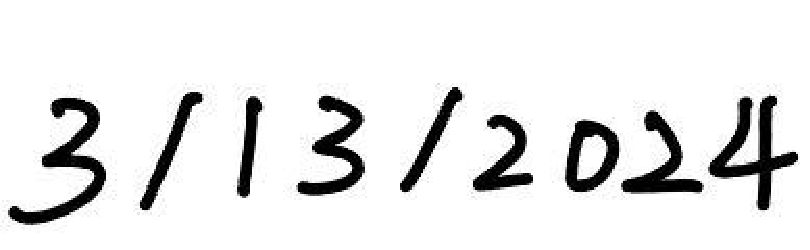
\includegraphics[width=40pt]{date.pdf}
    % }
}
% 老师的手写签名,signature.pdf 改为老师的手写签名文件名
\supervisorsignature{
    % \raisebox{-5pt}{
    
\includegraphics[width=40pt]{xuebai.pdf}
    % }
}
% 老师手写的时间,signature.pdf 改为老师的手写的日期文件名
\teachertime{
    % \raisebox{-5pSt}{
    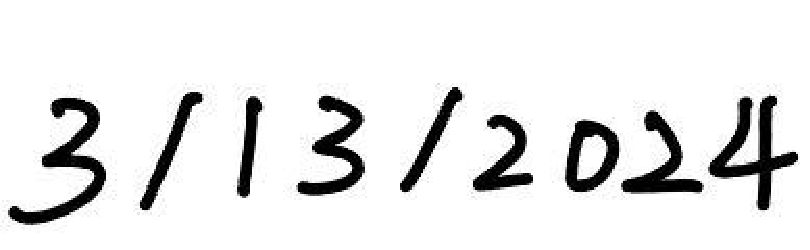
\includegraphics[width=40pt]{date.pdf}
    % }
}
% 老师手写的成绩
\recommendedgrade{
    % \raisebox{-5pt}{
    % \includegraphics[width=40pt]{}
    % }
}

\makestatement

%==============================%
% ↑ ↑ ↑ 诚信说明页 授权说明书
%==============================%


%=====%
%论文(设计)成绩:注意2007的模板要求,成绩页在最后,2021要求成绩页在摘要前面
%=====%

% 下面这些注释掉可以去掉成绩、评语什么的
\supervisorcomment{}


\committeecomment{}

\finalgrade{}
% 上面这些注释掉可以去掉成绩、评语什么的


\frontmatter



%中文摘要
\ZhAbstract{磁场的约束是一个非常重要的研究课题,但同时也是个十分复杂的问题;目前还没
有求解复杂磁场系统力学的解析方法,只能通过数值计算来求解,现有的数值积分算法主要有Monte Carlo 算法、
Adaptive complex Simpson 算法、Gauss 积分、Romberg积分等。 它们均存在优势与短板,同时在低算力
下也很难对这个问题进行求解。于是如何设计、优化算法就成了不可避免地问题。但通过实验
对永磁体在磁场约束下的复摆运动进行分析,可以给出一些定性的实验规律。}{磁场;复摆;数值分析}


%英文摘要
\EnAbstract{Magnetic field confinement is a very important research topic, but it is also a very complicated
problem. At present, there is no analytical method to solve the mechanics of complex magnetic
field systems, which can only be solved by numerical calculation, The main algorithm to slove this are 
Monte Carlo algorithm, Adaptive complex Simpson algorithm, Gauss Integral, Romberg Integral and so on.
All of them have their goods and shorts, and it is difficult to work when the arithmetic power is low.
so how to design the algorithm becomes an inevitable problem, and the existing numerical analysis methods are difficult to solve
this problem under low computational force. By analyzing the complex pendulum motion of
permanent magnet constrained by magnetic field, some useful qualitative experimental rules can be given.}
{magnetic field; complex pendulum; numerical analysis}

%生成目录
% \tableofcontents
% 下面这个包含图表目录
\customcontent


% % 部分同学需要专业术语注释表,* 表示不加入目录
% \chapter*{专业术语注释表}
% \begin{longtable}{lll}
%   \caption*{缩略词说明}\\
%   SS & Spread Spectrum & 扩展频谱 \\
%   PAPR & Peak to Average Power Ratio & 峰均比\\
%   DCSK & Differential Chaos Shift Keying &差分混移位键控\\
%   dasd & fdhfudw eqwrqw fasfasfs fewev wqfwefew &\tabincell{l}{太长了\\换行一下}\\
% \end{longtable}


%文章主体
\mainmatter

\chapter{\texorpdfstring{绪 \quad 论}{绪论}}
本课题选自2023年中国大学生物理学术竞赛第八题。题目的叙述如下:
\begin{center}
    \fbox{
        \parbox{.9\linewidth}{
        \centerline{\textbf{Euler's Pendulum 欧拉摆}}

        Take a thick plate of non-magnetic material and fix a neodymium magnet on top of it. Suspend 
        a magnetic rod (which can be assembled from cylindrical neodymium magnets) underneath it. Deflect 
        the rod so that it touches the plate only with highest edge and release it. Study the motion of such 
        a pendulum under various conditions.

        取一块厚的、无磁性材料制成的板,并在其上面固定一个钕磁铁。在板的下方悬挂一根磁性杆(可以由多块圆柱形钕磁铁组装制成)。
        使杆偏转至它只有最顶部的边沿接触到板,然后将其释放。研究这种摆在各种条件下的运动。
        }
    }
\end{center}
项目以此题为基础,探究了磁场约束下永磁体棒的运动,得到了棒的复摆运动周期与磁场分布、棒的长度
和介质板厚度的定性关系,比提供了大量数据,为经验公式的创建提供了必要支持。

对于复杂系统的求解目前没有解析解法,只能使用数值算法。项目从最基本的Biot–Savart 定律出发建立
微分方程,通过数值积分的方式求解,得到了磁场在空间中的分布。通过COMSOL仿真软件模拟物理场,得出了
在棒长较短时与试验相符合的结果。

通过文献调研,在此之前没有任何相关文献记载此类问题的研究,项目建立在自主创新的基础上对此问题
进行了较为全面的探究。

本文的主要内容分为一下几个方面:

第二章具体推导了永磁体的磁场分布以及受力情况,并给出了数值算法的基本思路。同时也考虑了相关
因素对于本试验的影响。

第三章给出了预实验的基本方法以及得到的结果。为正式实验找寻到了更为合适的方式。

第四章介绍了正式实验的过程、数据的具体分析以及从数据及实验过程中可以得到的结论。同时介绍了
项目组在实验中发明的一种比较实用的一种准直方法——“滚动准直法”。

第五章根据实验的各类参数设计了数值算法计算了磁场的分布,同时进行了物理场仿真模拟,对问题的
感悟有了进一步加深。

最后第六章对整个项目进行回顾、总结与展望。

\chapter{理论分析}
\section{磁场}
Biot-Savart law\cite{Biot_Savart_Law}是描述恒定电流产生的磁场的方程,这是一个近似方程。
因为根据量子力学,磁性起源于轨道电流和自旋电流且自旋电流占有很大一部分。但是其与安培定律和高斯定理
是相容的,可以说其实磁场近似计算非常好的方程。本项目以此定律为基础建立了永磁体的磁场分布
方程。

总体来说,形状及充磁方向一致的永磁体磁场分布大致相同,不同的是相对强度的大小。对于圆柱体永磁体,假设其
磁化电流均匀分布在侧面,磁化电流密度为$i^{'}$。运用毕奥-萨伐尔定律来计算磁场的空间分布。
\begin{figure}[H]
    \centering
    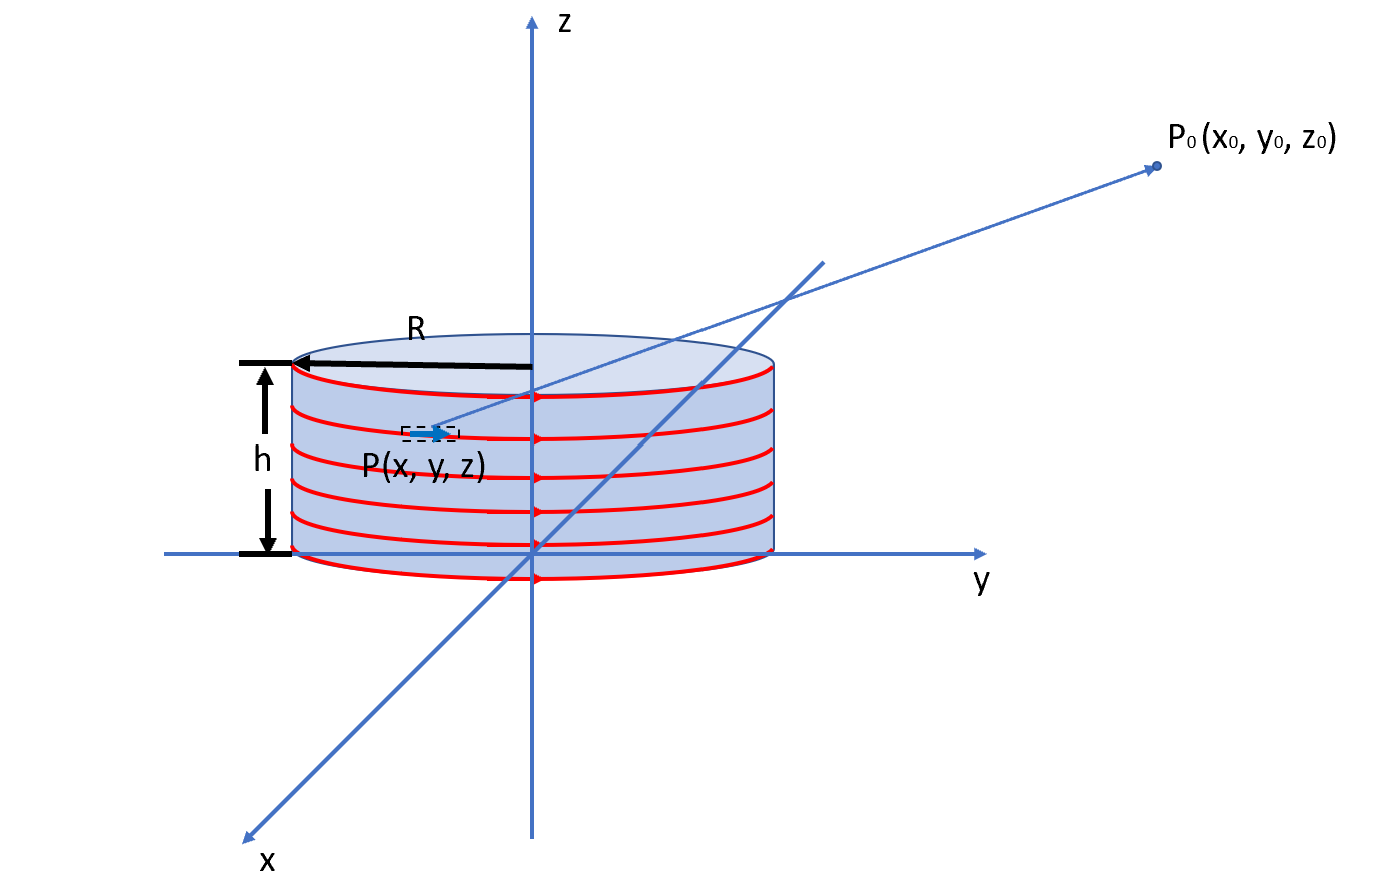
\includegraphics[width=0.6\textwidth]{figures/magneticfield.png}
    \caption{magneticfield}
    \label{magneticfield}
\end{figure}
Biot-Savart 定律的微分形式(考虑磁介质)为:
\begin{equation}
    d\mathbf {B} (\mathbf {r} )={\frac {\mu}{4\pi }}{\frac {I\,d{\boldsymbol {\ell }}\times \mathbf {r'} }{|\mathbf {r'} |^{3}}}
\end{equation}
在图\ref{magneticfield}中:
\begin{equation}
    \begin{aligned}
        & \quad \mathbf{r} = (x_0 - x, y_0 - y, z_0 - z)\\
        & \quad d\boldsymbol {\ell } = (dx, dy, 0)
    \end{aligned}
\end{equation}

因此:
\begin{equation}
    d\boldsymbol {\ell } \times \mathbf{r} = \left | \begin{matrix}
    \mathbf{i} &\mathbf{j}   &\mathbf{k} \\
    dx &dy &0  \\
    x_0 - x & y_0 - y &z_0 - z \\
    \end{matrix} \right |  = (z_0 - z)dy\mathbf{i} - (z_0 - z)dx\mathbf{j} + 
    [(y_0 - y)dx - (x_0 - x)dy]\mathbf{k}
\end{equation}

对$x, y, z$使用极坐标表示,并带入上式,就可以得到$P_{0}$点的磁感应分量:
\begin{equation}
    \begin{aligned}
        & \quad
        \left  \{
        \begin{array}{lr}
        x = Rcos\theta, & 0\leq \theta \leq 2\pi \\
        y = Rsin\theta, & 0\leq \theta \leq 2\pi \\
        z = z, & 0\leq z \leq h\\
        K = [(x_0 - Rcos\theta)^2 + (y_0 -Rsin\theta)^2 + (z_0 - z)^2]^\frac{3}{2}
        \end{array}
        \right.\\
        & \quad
        \left \{
        \begin{array}{lr}
        B_x = \frac{\mu_0i^{'}}{4\pi} \int_{0}^{h}\int_{0}^{2\pi} \frac{(z_0 - z)Rcos\theta}{K} \,d\theta\,dz & \\
        B_y = \frac{\mu_0i^{'}}{4\pi} \int_{0}^{h}\int_{0}^{2\pi} \frac{(z_0 - z)Rsin\theta}{K} \,d\theta\,dz & \\
        B_z = \frac{\mu_0i^{'}}{4\pi} \int_{0}^{h}\int_{0}^{2\pi} \frac{-(y_0 - Rsin\theta)Rsin\theta -(x_0 - Rcos\theta)Rcos\theta}{K} \,d\theta\,dz & \\
        \end{array}
        \right.\\
        & \quad
        I = i^{'}\text{d}z
    \end{aligned}
\end{equation}

经调查\cite{圆柱形永磁体磁场建模及仿真研究}:
\begin{equation}
    i^{'} = \frac{B_{\gamma}}{\mu_{0}}
\end{equation}
其中,$B_{\gamma}$是剩余磁化强度,这是永磁体的一个参数。

\section{平面复摆运动}
\subsection{可行性推导}
对于项目研究的系统,介质板可以被视为是无限大的,这样磁场就是轴对称的。如图\ref{force_on_currentloop},取任意关于运动
平面(假设它是平面运动,只要没有垂直于平面的分力,摆动就是在平面内的,即假设成立)位置对称的电流元$Id\boldsymbol {\ell }_1 = I(x_0, y_0, z_0)$,
$Id\boldsymbol {\ell }_2 = I(x_0, -y_0, -z_0)$,这两点处的磁感应强度分别为$B_1 = (B_x, B_y, B_z)$,$B_2 = (-B_x, B_y, B_z)$。我们可以
得到$Id\boldsymbol {\ell }_1 \times B_1 + Id\boldsymbol {\ell }_2 \times B_2 = 0\mathbf{i} + 2(z_0B_x-x_0B_z)\mathbf{j} + 2(x_0B_y-y_0B_x)\mathbf{k}$。
所以棒是可以在平面运动的。
\begin{figure}[H]
    \centering
    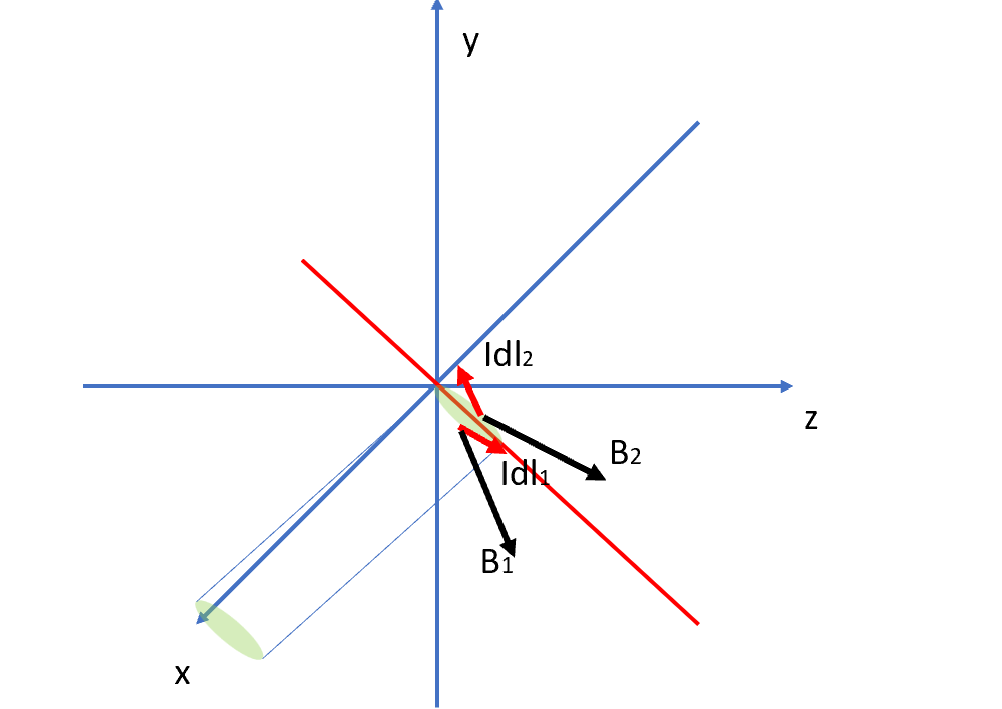
\includegraphics[width=8cm]{force_on_currentloop.png}
    \caption{force on currentloop}
    \label{force_on_currentloop}
\end{figure}

\subsection{顶点位置}
上面的推导是建立在开始时棒的轴与磁铁的轴重合的基础上的,但这是有条件的。只有当介质板的厚度达到一定程度才可以实现。
实验上可以得到这个结果,在第四章中项目组对磁场进行参数绘制,定性给出了这个结果。

\subsection{转动惯量}
转动惯量可用定义及平行轴定理算出,如图\ref{rotation_interia}:
\begin{figure}[H]
    \centering
    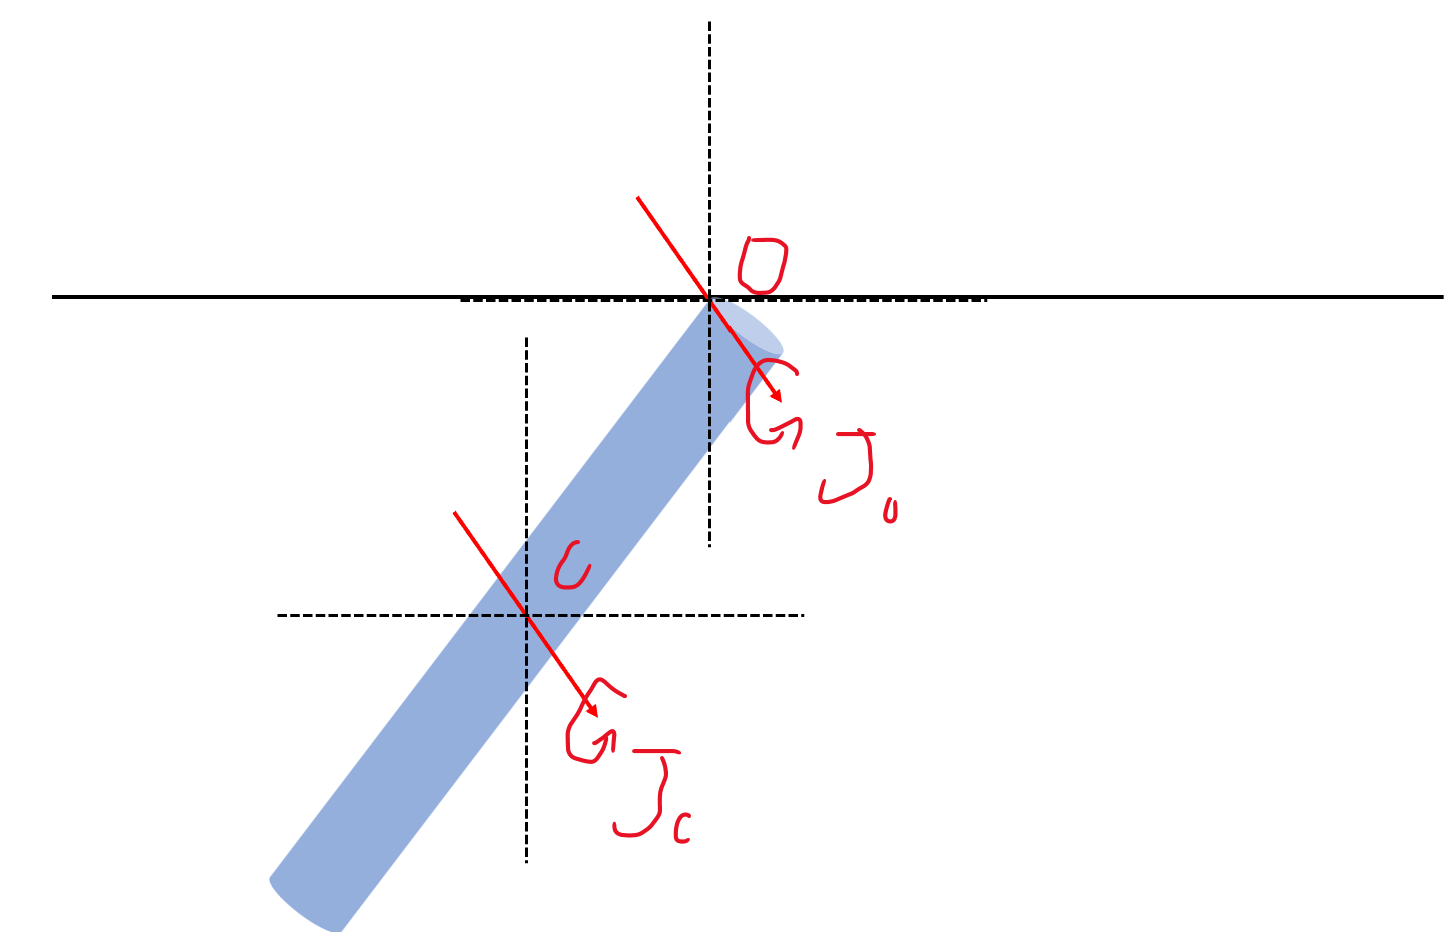
\includegraphics[width=8cm]{rotation_interia.png}
    \caption{rotation interia}
    \label{rotation_interia}
\end{figure}
设棒的半径为R,长为l,密度均匀且为$\rho$,质量$m = \rho\pi R^2l$。则:
\begin{equation}
    \begin{aligned}
    J_c &= \int\int\int_{\Omega} (x^2+y^2)\rho \,dx\,dy\,dz\\
    &= \rho\int_{-\frac{l}{2}}^{\frac{l}{2}}\int_{-R}^{R}\int_{-\sqrt{R^2-x^2}}^{\sqrt{R^2-x^2}} (x^2+y^2) \,dz\,dx\,dy\\
    &= \rho\pi R^2l(\frac{R^2}{4}+\frac{l^2}{12})\\
    &= m(\frac{R^2}{4}+\frac{l^2}{12})\\
    \end{aligned}
\end{equation}

于是:
\begin{equation}
\begin{aligned}
J_o = m(\frac{5R^2}{4}+\frac{l^2}{3})
\end{aligned}
\end{equation}

\subsection{运动方程}
\begin{figure}[H]
    \centering
    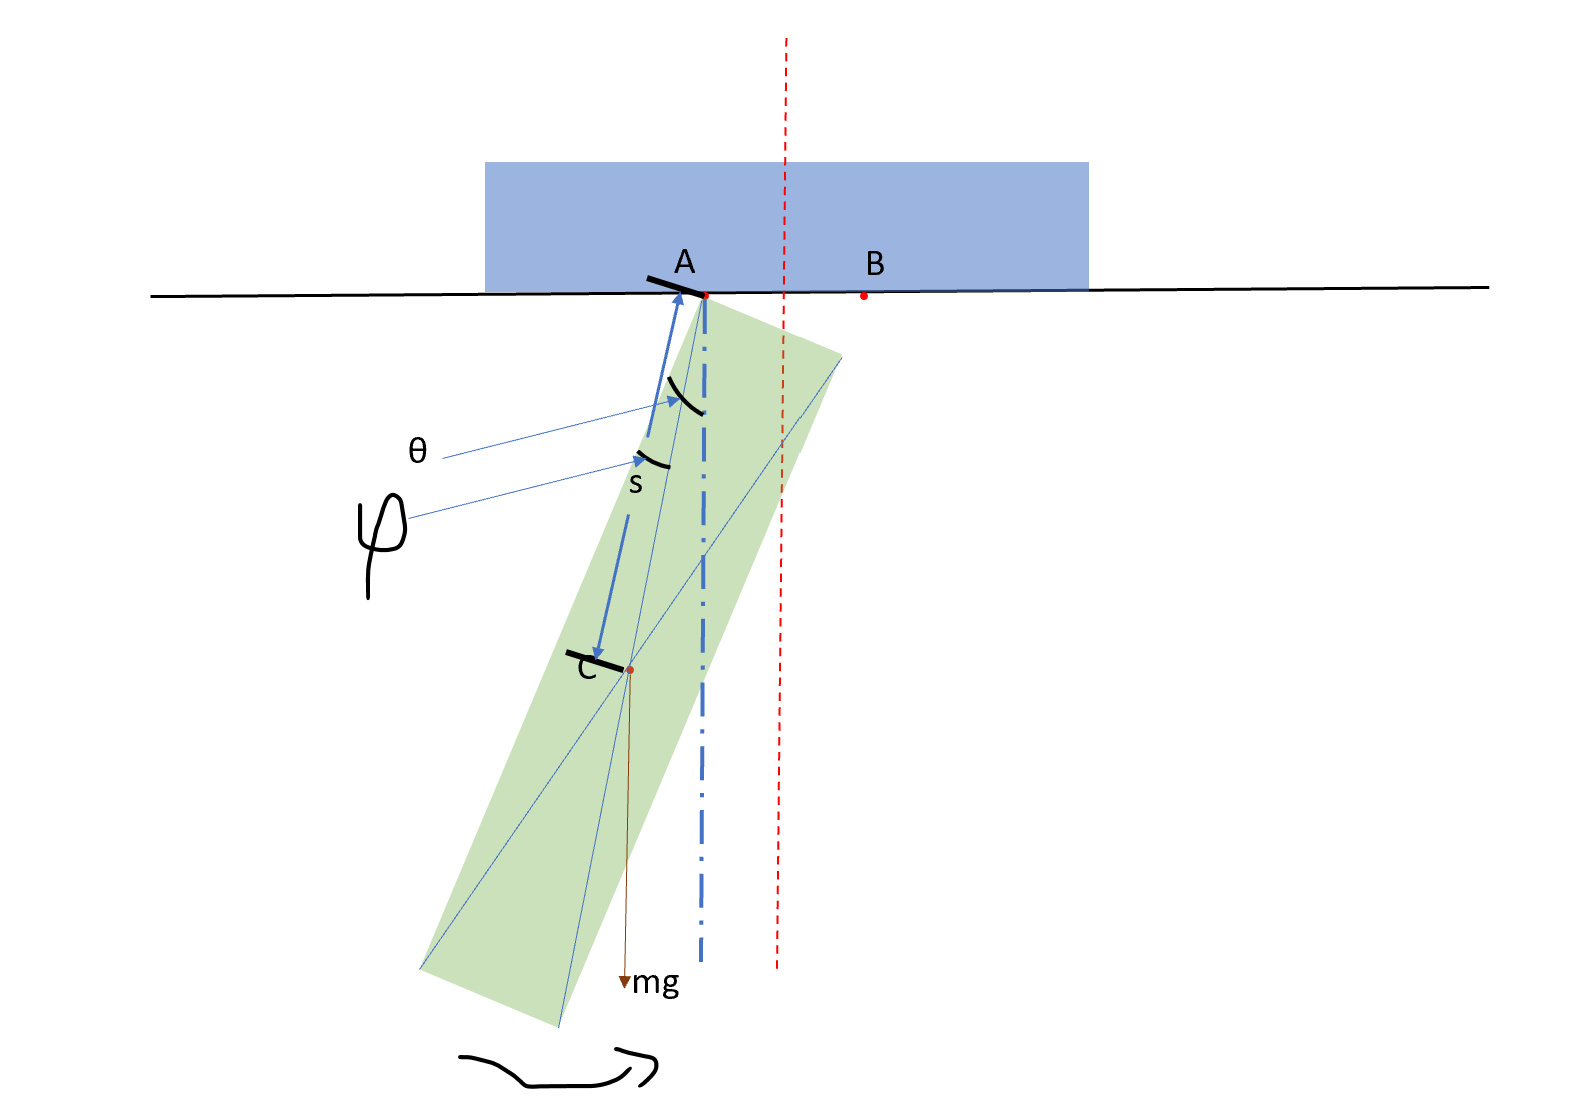
\includegraphics[width=8cm]{equation_of_motion.png}
    \caption{equation of motion}
    \label{equation_of_motion}
\end{figure}
要求运动的微分方程,首先要知道受力,其中比较困难的是阻力和磁场力。先分析阻力,一般的处理方法是认为阻力与速度成正比,
这里用角速度,与棒有关的那个常数(由受力面积、形状等决定)计入阻力系数,记为$\gamma$,则$f = \gamma \frac{d\theta}{dt}$。

对于磁场力,只能做定性分析,给出解析式比较困难。根据对称性,磁场力是$\theta$的周期函数。
可以设为$\mu(\theta-\varphi)$。加上重力,记为$F(\theta) = mgsin(\theta-\varphi)+\mu(\theta-\varphi)$。
其中$\theta$、$\varphi$的物理意义如图\ref{equation_of_motion}。

考虑$\frac{1}{4}$周期,因为这里涉及到一个碰撞问题,如图\ref{collision}:
\begin{figure}[H]
    \centering
    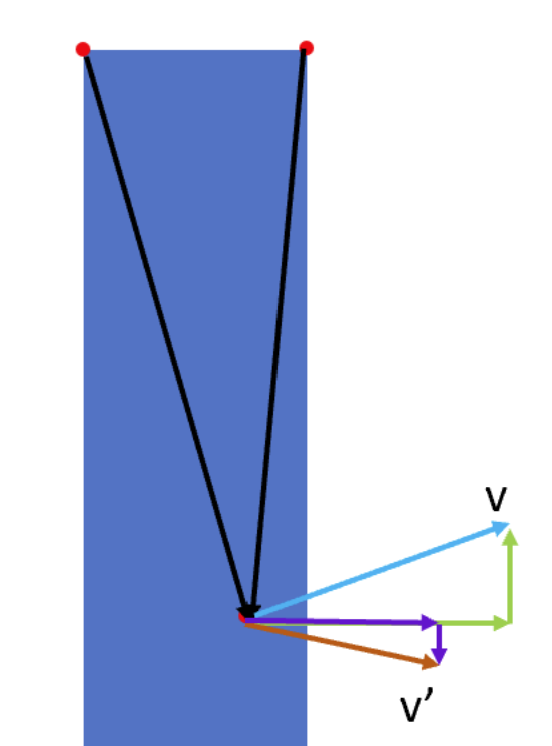
\includegraphics[width=4cm]{collision.png}
    \caption{collision}
    \label{collision}
\end{figure}
可以预想,在棒在与介质板接触的两个顶点(图\ref{collision}中红色的点)切换的瞬间会有一个与介质板的碰撞,假设这个碰撞会使垂直于板的动量分量损失;而水平方向上,
也会由于摩擦力的作用而使水平动量发生改变。这是必须的,因为要保证质点与顶点的连线与速度方向垂直。这两者的变化并不是独立的,
主导作用是垂直方向,因为摩擦力是约束力,它应响应垂直方向的速度变化(但这也包含了一个摩擦力的临界问题,棒和介质板之间可能会有相对滑动)。于是,
假设它可以类比于一维的碰撞,有个恢复系数e,这样就可以通过观察摆幅的变化来判断e的大小,当然,前提是得到势场的空间分布,
因为是磁场和重力场耦合,所以这会复杂一些。

对于图\ref{equation_of_motion},由转动定理:
\begin{equation}
    \begin{aligned}
    J_0\frac{\mathrm{d}^{2} \theta }{\mathrm{d} t^{2}} + \gamma\frac{\mathrm{d} \theta}{\mathrm{d} t} + F(\theta) = 0
    \end{aligned}
\end{equation}

对于小角度(摆动的后期),可以近似$sin(\theta - \varphi) = \theta - \varphi$,同时令$\theta - \varphi = \phi$,得到下列方程:
\begin{equation}
    \begin{aligned}
    J_0\frac{\mathrm{d}^{2} \phi }{\mathrm{d} t^{2}} + \gamma\frac{\mathrm{d} \phi}{\mathrm{d} t} + mgs\phi = -\mu(\phi)
    \end{aligned}
\end{equation}

解为:
\begin{equation}
    \begin{aligned}
    \phi = \left  \{
    \begin{array}{lr}
    C_1e^{r_1t}+C_2e^{r_2t}-e^{r_1t}\int \frac{U_{21}\mu(\phi)}{detU}\,d\phi-e^{r_2t}\int \frac{U_{22}\mu(\phi)}{detU}\,d\phi, &r_1\neq r_2 \\
    (C_1+C_2t)e^{rt}-e^{rt}\int \frac{U_{21}\mu(\phi)}{detU}\,d\phi-te^{rt}\int \frac{U_{22}\mu(\phi)}{detU}\,d\phi, &r_1 = r_2 = r
    \end{array}
    \right.
    \end{aligned}
\end{equation}
其中,$r_1 = (-P+\sqrt{P^2-4Q})/2, r_2 = (-P-\sqrt{P^2-4Q})/2, P = \frac{\gamma}{J_0}, Q = \frac{mgs}{J_0}$,

$U = \left \{
\begin{array}{lr}
\left[
\begin{matrix}
    e^{r_1t} &e^{r_2t} \\
    r_1e^{r_1t} &r_2e^{r_2t}
\end{matrix} \right], &r_1\neq r_2 \\


\left[
\begin{matrix}
    e^{rt} &te^{rt} \\
    re^{rt} &(1+rt)e^{rt}
\end{matrix}\right], &r_1 = r_2 = r
\end{array}
\right.$,$U_{ij}$是U的代数余子式。

上面的方程用来计算是比较困难的,下面进行简化:

假设能量的损失主要发生在碰撞上面,忽略空气阻力等阻尼,于是我们给出运动方程:
\begin{equation}
    J_{0}*\frac{d^{2}\alpha}{dt^{2}} + F_{L}(\alpha) = 0
\end{equation}
其中$J_{0}$已由上面计算给出,为$m(\frac{5R^2}{4} + \frac{l^2}{3})$。

下面将给出$F_{L}(\alpha)$,如图\ref{force}:
\begin{figure}[H]
    \centering
    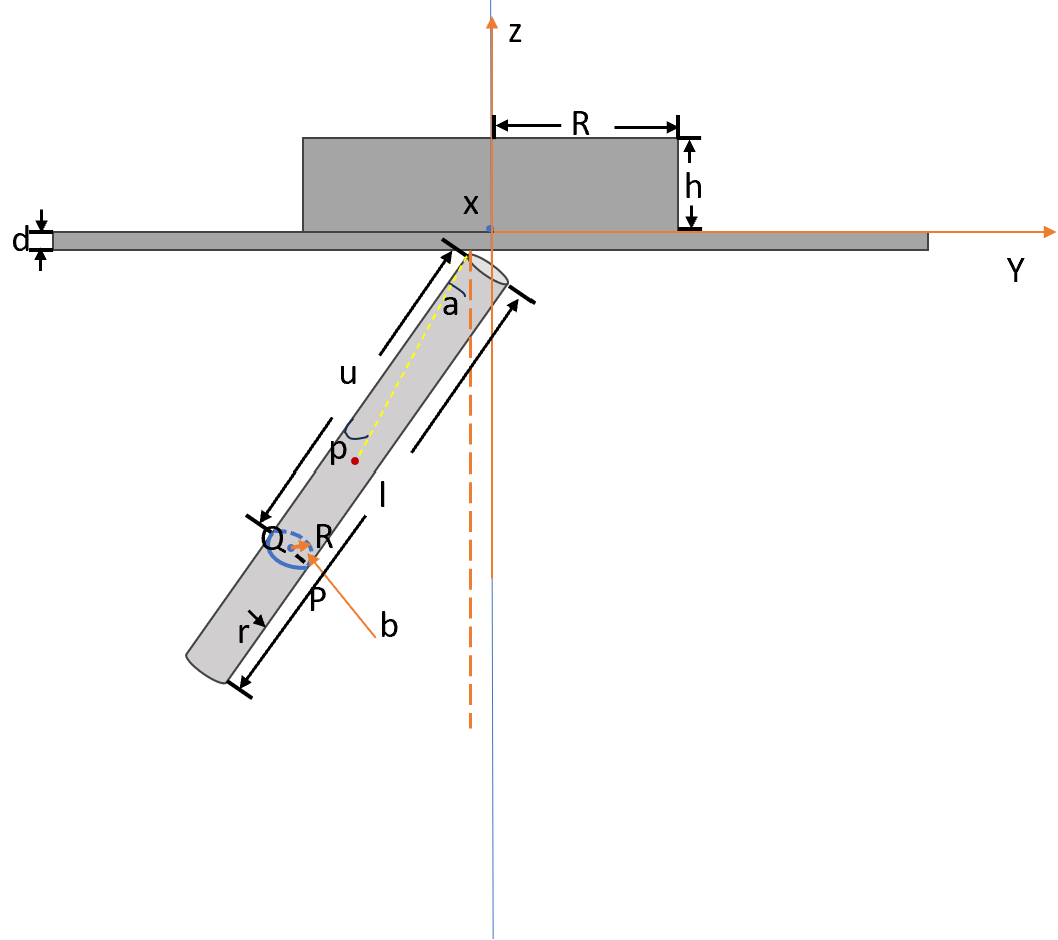
\includegraphics[width=8cm]{figures/force.png}
    \caption{force}
    \label{force}
\end{figure}

用x,y,z来代替$x_{0},y_{0},z_{0}$,z用w代替,则磁场为:
\begin{equation}
    \left \{
    \begin{array}{lr}
    B_x = \frac{\mu_0i^{'}}{4\pi} \int_{0}^{h}\int_{0}^{2\pi} \frac{(z - w)Rcos\theta}{K} \,d\theta\,dw & \\
    B_y = \frac{\mu_0i^{'}}{4\pi} \int_{0}^{h}\int_{0}^{2\pi} \frac{(z - w)Rsin\theta}{K} \,d\theta\,dw & \\
    B_z = \frac{\mu_0i^{'}}{4\pi} \int_{0}^{h}\int_{0}^{2\pi} \frac{-(y - Rsin\theta)Rsin\theta -(x - Rcos\theta)Rcos\theta}{K} \,d\theta\,dw & \\
    \end{array}
    \right.
\end{equation}
其中,$K = [(x - Rcos\theta)^2 + (y -Rsin\theta)^2 + (z - w)^2]^\frac{3}{2}$

P点的坐标:
$P(0, r+\mu sin\alpha, -d-\mu cos\alpha)$

同理,$Q(0, r+\mu sin\alpha-r*cos\alpha, -d-\mu cos\alpha -r*sin\alpha)$

$R(r*sin\alpha, r+\mu sin\alpha-r*cos\alpha+r*cos\beta*cos\alpha, -d-\mu cos\alpha -r*sin\alpha+r*cos\beta*sin\alpha)$

$\textbf{dl} = (r*cos\beta, -r*sin\beta*cos\alpha, -r*sin\beta*sin\alpha)*d\beta$

于是,
\begin{equation}
\left \{
\begin{array}{lr}
F_x = i^{''}*\int_{0}^{l}\int_{0}^{2\pi}  (dl_{y} \times B_{z} - dl_{z} \times B_{y})\,d\beta\,du & \\
F_y = i^{''}*\int_{0}^{l}\int_{0}^{2\pi}  (dl_{z} \times B_{x} - dl_{x} \times B_{z})\,d\beta\,du & \\
F_z = i^{''}*\int_{0}^{l}\int_{0}^{2\pi}  (dl_{x} \times B_{y} - dl_{y} \times B_{x})\,d\beta\,du & \\
\end{array}
\right.
\end{equation}

由上面的对称性分析可以得到$F_{x} = 0$,于是$F_{L}(\alpha) = i^{''}*\int_{0}^{l}\int_{0}^{2\pi}  
z*(dl_{z} \times B_{x} - dl_{x} \times B_{z}) + y*(dl_{x} \times B_{y} - dl_{y} \times B_{x})\,
d\beta\,du -mg(\frac{l}{2}*cos\alpha + r*sin\alpha)$

于是角加速度为
\begin{equation}
    \frac{d^{2}\alpha}{dt^{2}} = -\frac{F_{L}(\alpha)}{J_{0}}
    =-\frac{i^{'}*i^{''}}{J_{0}}*\frac{F_{L}(\alpha)}{i^{'}*i^{''}} + \frac{g}{\frac{5R^2}{4} + \frac{l^2}{3}}*(\frac{l}{2}*cos\alpha + r*sin\alpha)
\end{equation}
未知量有恢复系数e。($\alpha_{0}$为90度)。

这个积分非常复杂,它是两个二重积分的结合,用数学软件可以给出数值解,但却无法给出运动方程的解,
但是可以通过迭代算法来进行周期的求解。离散化可以用下面的方程组表示。根据实验得到的数据,
可取$\psi = 0.001s$。

\begin{equation}
    \left \{
    \begin{array}{lr}
    \alpha(t+\psi) = \alpha(t) + \psi*w(t+\psi /2) & \\
    w(t+\psi /2) = w(t-\psi /2) + \psi*\beta(t) & \\
    \beta(t) =\beta(\alpha(t)) & \\
    \alpha(0) = 90 & \\
    w(\psi /2) = w(0) + \psi /2*\beta(0) & \\
    \end{array}
    \right.
\end{equation}

\section{圆锥摆}

除了复摆这种简单的运动形式外,还有圆锥摆这种运动形式。实验上可以观察到两种圆锥摆的摆动
形式——1.接触点不动。2.接触点做圆周运动。对于这两种圆锥摆动形式,都可以根据向心力公式
$F_c = \int_{\Omega} \rho\omega^2r \,d\Omega$,其中$\Omega$表
示棒占据的空间,来计算圆锥摆在稳定时的位置。而这只是在理想条件下的;对接触点
做圆周运动的摆动形式,受力得是对称的,这要求转轴与上方磁铁的轴共线。对于顶点
不变的摆动,可能存在也可能不存在这样的位置。由于器材等的限制,本项目未对此问题做进一步的研究。

\section{其他摆动形式及因素}
上述的摆动形式是在理想的情况下才能观察到,实际很难看到;下面将定性分析实际中的复杂摆动。

\subsection{进动、章动与过渡}
由于棒与板之间存在摩擦,摆动的能量就会损耗,这会使圆锥摆向复摆过渡;这种过渡的结果就是产生了进动和章动。
因为圆锥摆会退化为平面的摆动,但它很难达到不偏离轴平面(我们定义通过轴的复摆摆动平面为轴平面),于是根据上面的受力分析,
会有一个指向轴的磁场力,这会产生一个力矩,这个力矩的作用效果就是使棒进动。但如果它大了或小了,那么就变成了章动。

\subsection{微小因素}
除了重力、磁力等比较大的影响因素外,还有许多微小的影响因素,这里列举三个。

第一,地磁场的作用。这个在要求精度不高的情况下可以忽略。地磁场的大小为$0.5-0.6Gs$,
而钕磁铁一般为$12200-14800Gs$,相比之下,可以忽略地磁。

第二,科氏力。由于地球是非惯性系,棒在运动过程中会受到科氏力的作用。我们取最大的角度使$F_k = 2v\omega$,
这样近似结果约为$10^{-4}N$。实验上,在控制无垂直于振动面的速度情况下,摆顺逆时针进动出现
的概率近似相等。说明科氏力的影响比较小。

第三,电磁感应。在棒摆运动的过程中,它产生的磁场会反复磁化介质板和上方磁铁,这会产生电磁波损耗能量。
但实际上它非常小,可以忽略其对实验的影响。

\subsection{其他}
上面考虑的是上方圆柱形磁铁的情形,形状不同的磁铁只需重新计算磁场即可,其他可以类比。对于顶点的位置,
实际上在摆动过程中其并不是固定的。而像板的厚度,材料,棒的长度等影响因素其实包含在了微分
方程中,它们是作为参数的形式起作用的。

\chapter{预实验及其结果}
\section{实验装置}
如图\ref{magnet}是实验中用到的磁铁,其中较长的是作为棒的,还有两个与之相同的,可以拼接在
一起以改变棒长。
\begin{figure}[H]
    \centering
    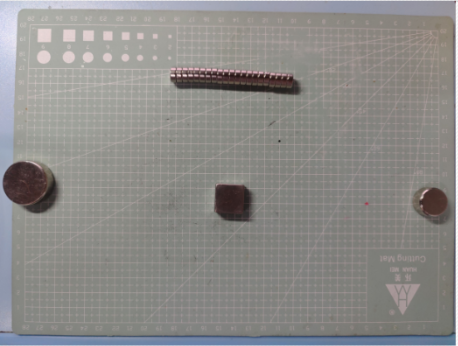
\includegraphics[width=8cm]{figures/magnet.png}
    \caption{magnet}
    \label{magnet}
\end{figure}

对于实验中用到的器材的参数请见附录\ref{参数}中的表\ref{实验器材参数}。

预实验的实验平台比较简陋,亚克力板是由两个铁架台夹住的。但这不影响预实验的总体效果。

\section{实验方法}
项目考虑到数据的收集方式对实验结果会有一定的影响,于是在与实验中对比了两种方法——
1.摄像法。以手机摄像功能对实验过程进行录像,后续通过视频处理软件数出两个“周期”的周期的
帧数,进而得出周期的大小。2.声波法。通过手机记录摆动过程中的音频数据,由于棒和板碰撞的过程中
响度较大,所以可以通过声波振幅谱中峰值的时间间隔得出周期。
\begin{figure}[H]
    \centering
    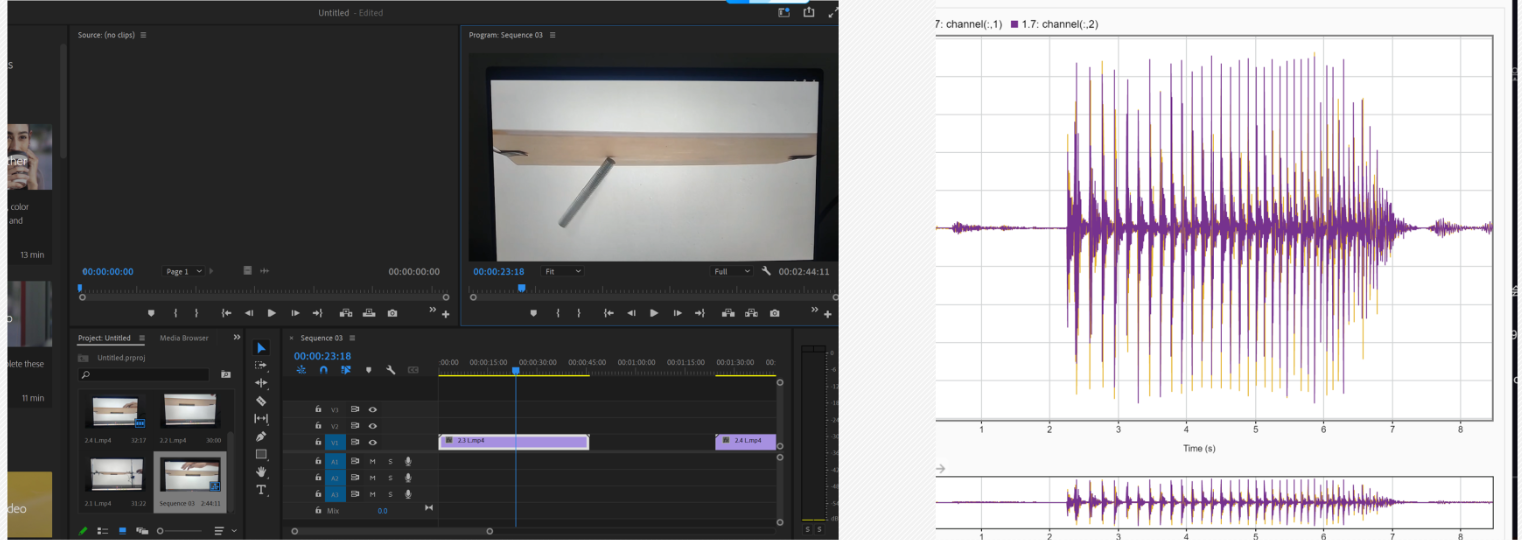
\includegraphics[width=11cm]{figures/ways.png}
    \caption{摄像法(左)和声波法(右)}
    \label{ways}
\end{figure}

两种方法均有一个共同的缺点——无法准确判断碰撞的时刻。但是通过实验得到
声波法的稳定性和可操作性较摄像法更好,如图\ref{data_ways}。因此选择其作为
正式实验的实验方法。

\begin{figure}[H]
    \centering
    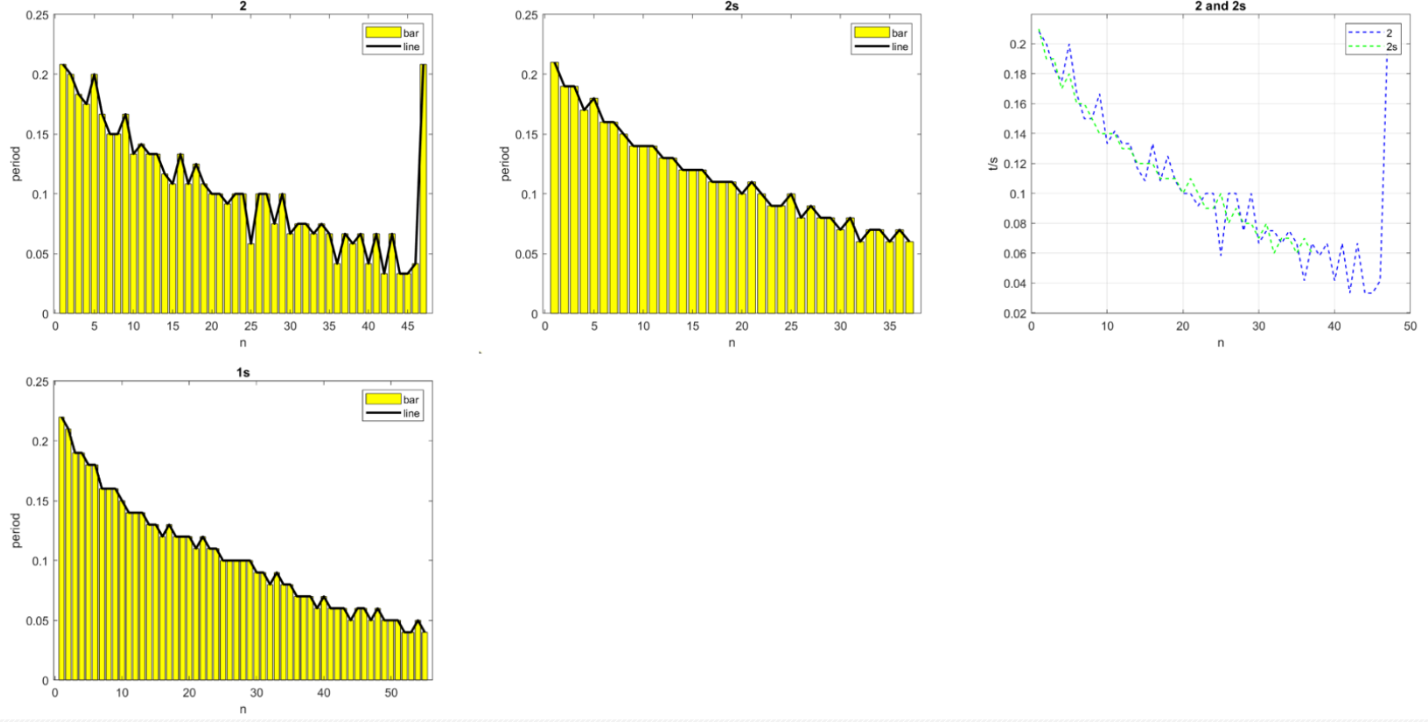
\includegraphics[width=11cm]{figures/data_ways.png}
    \caption{两种方法的实验结果}
    \label{data_ways}
\end{figure}

\section{结论}

\begin{itemize}
    \item 介质板只有在厚度不是太小时,才能使轴线成为一个稳定的平衡点。

    \item 比较预实验采用的两种数据处理方法,声波法处理误差更小,实验数据相对稳定。 

    \item 随着倾角的减小,摆的周期递减;当角度小到一定程度时,摆周期将会迅速减小为零。

    \item 控制相关因素,摆顺逆时针摆动都会出现,说明科氏力影响较小。 
\end{itemize}



\chapter{正式实验以及结果分析}
\section{实验装置}
实验装置如图\ref{equ},实验中发现亚克力板晃动较为剧烈,因此在板的两边加了重物以保证板
不会剧烈震动,图中并未体现。同时图中的电源是用以控制磁铁释放的装置。其连接一个电磁铁。
\begin{figure}[H]
    \centering
    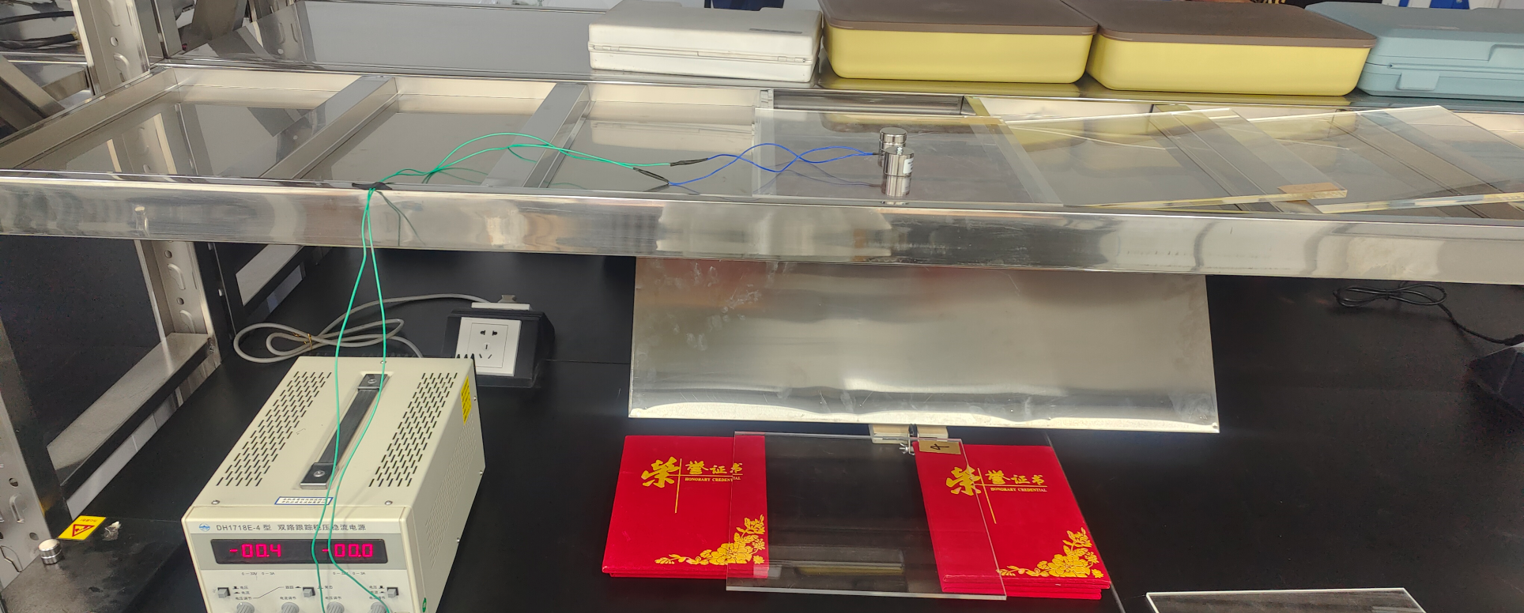
\includegraphics[width=12cm]{figures/eq.png}
    \caption{实验装置}
    \label{equ}
\end{figure}

\section{实验方法}
实验中发现由小磁铁拼成的磁棒不是严格共轴的,因此项目组想到了如图\ref{a_way}方法进行准直。
并称为“滚动准直法”。
\begin{figure}[H]
    \centering
    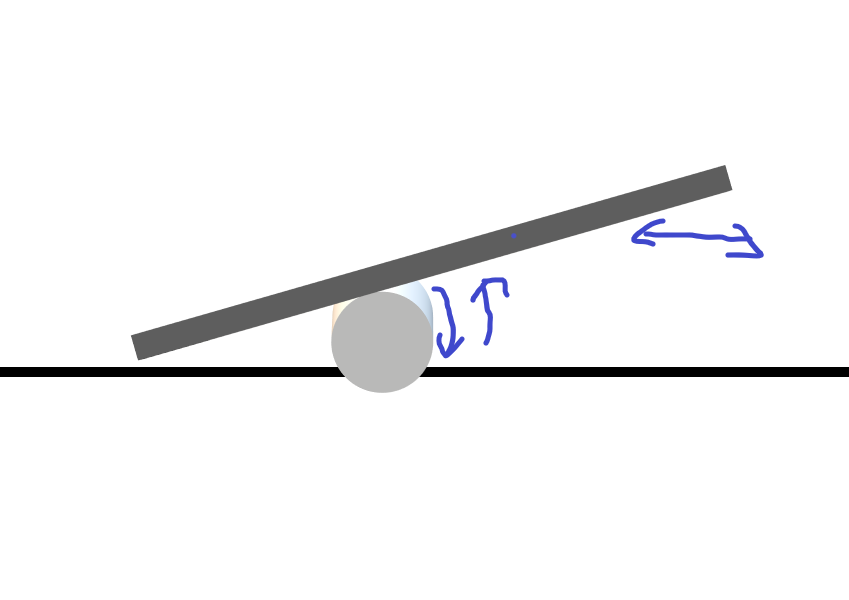
\includegraphics[width=8cm]{figures/a_way.png}
    \caption{滚动准直法}
    \label{a_way}
\end{figure}

\section{实验数据以及分析}
具体实验数据以及命名规则见附录\ref{实验数据}中的表\ref{数据}。其中数值按列排布,代表两次碰撞之间的时间间隔。

现对数据做如下分析:

实验对下同条件下的摆动进行三次测量,测量结果如图\ref{re}。
\begin{figure}[H]
    \centering
    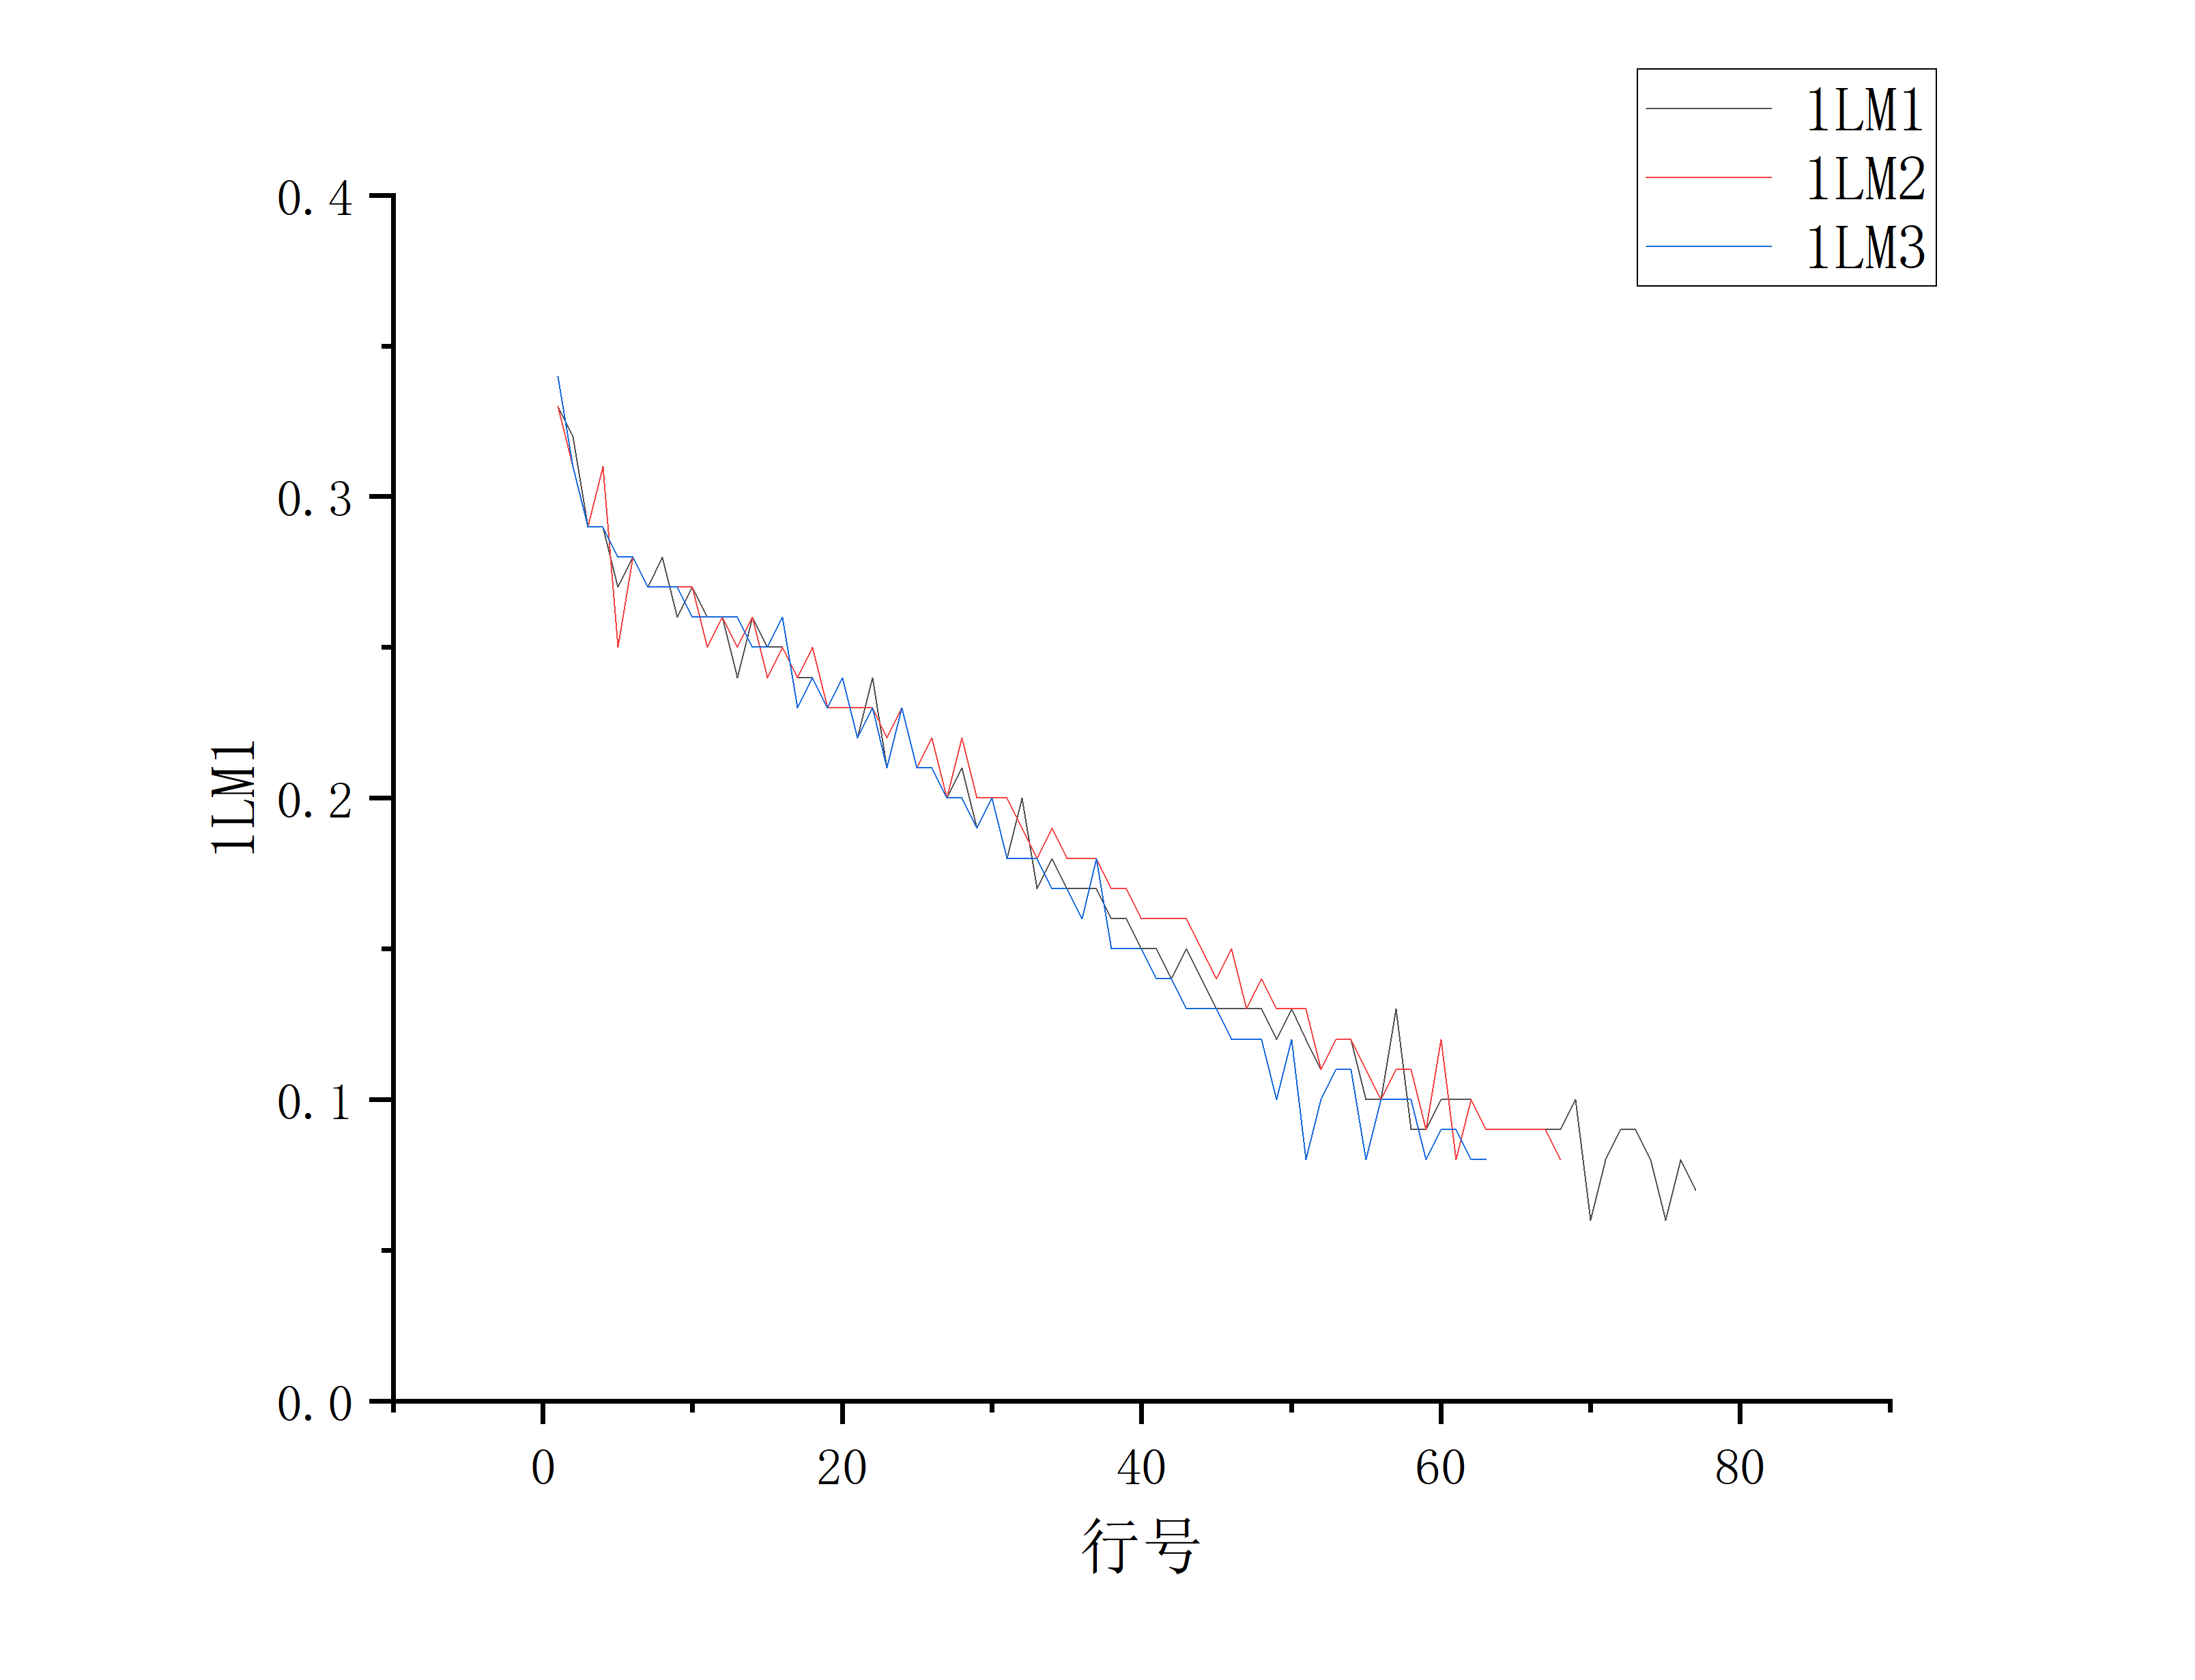
\includegraphics[width=12cm]{figures/重复性.png}
    \caption{重复性实验}
    \label{re}
\end{figure}

可见,实验具有良好的可重复性。

见图\ref{总体数据拟合},周期的衰减趋势更加趋向于2次(一次的$R^{2} \approx 0.96$,而
二次的$R^{2} \approx 0.99$)。但如果考虑具体计算的话,线性拟合会比较有优势。
\begin{figure}[H]
    \centering
    \subfloat[拟合次数1]{
        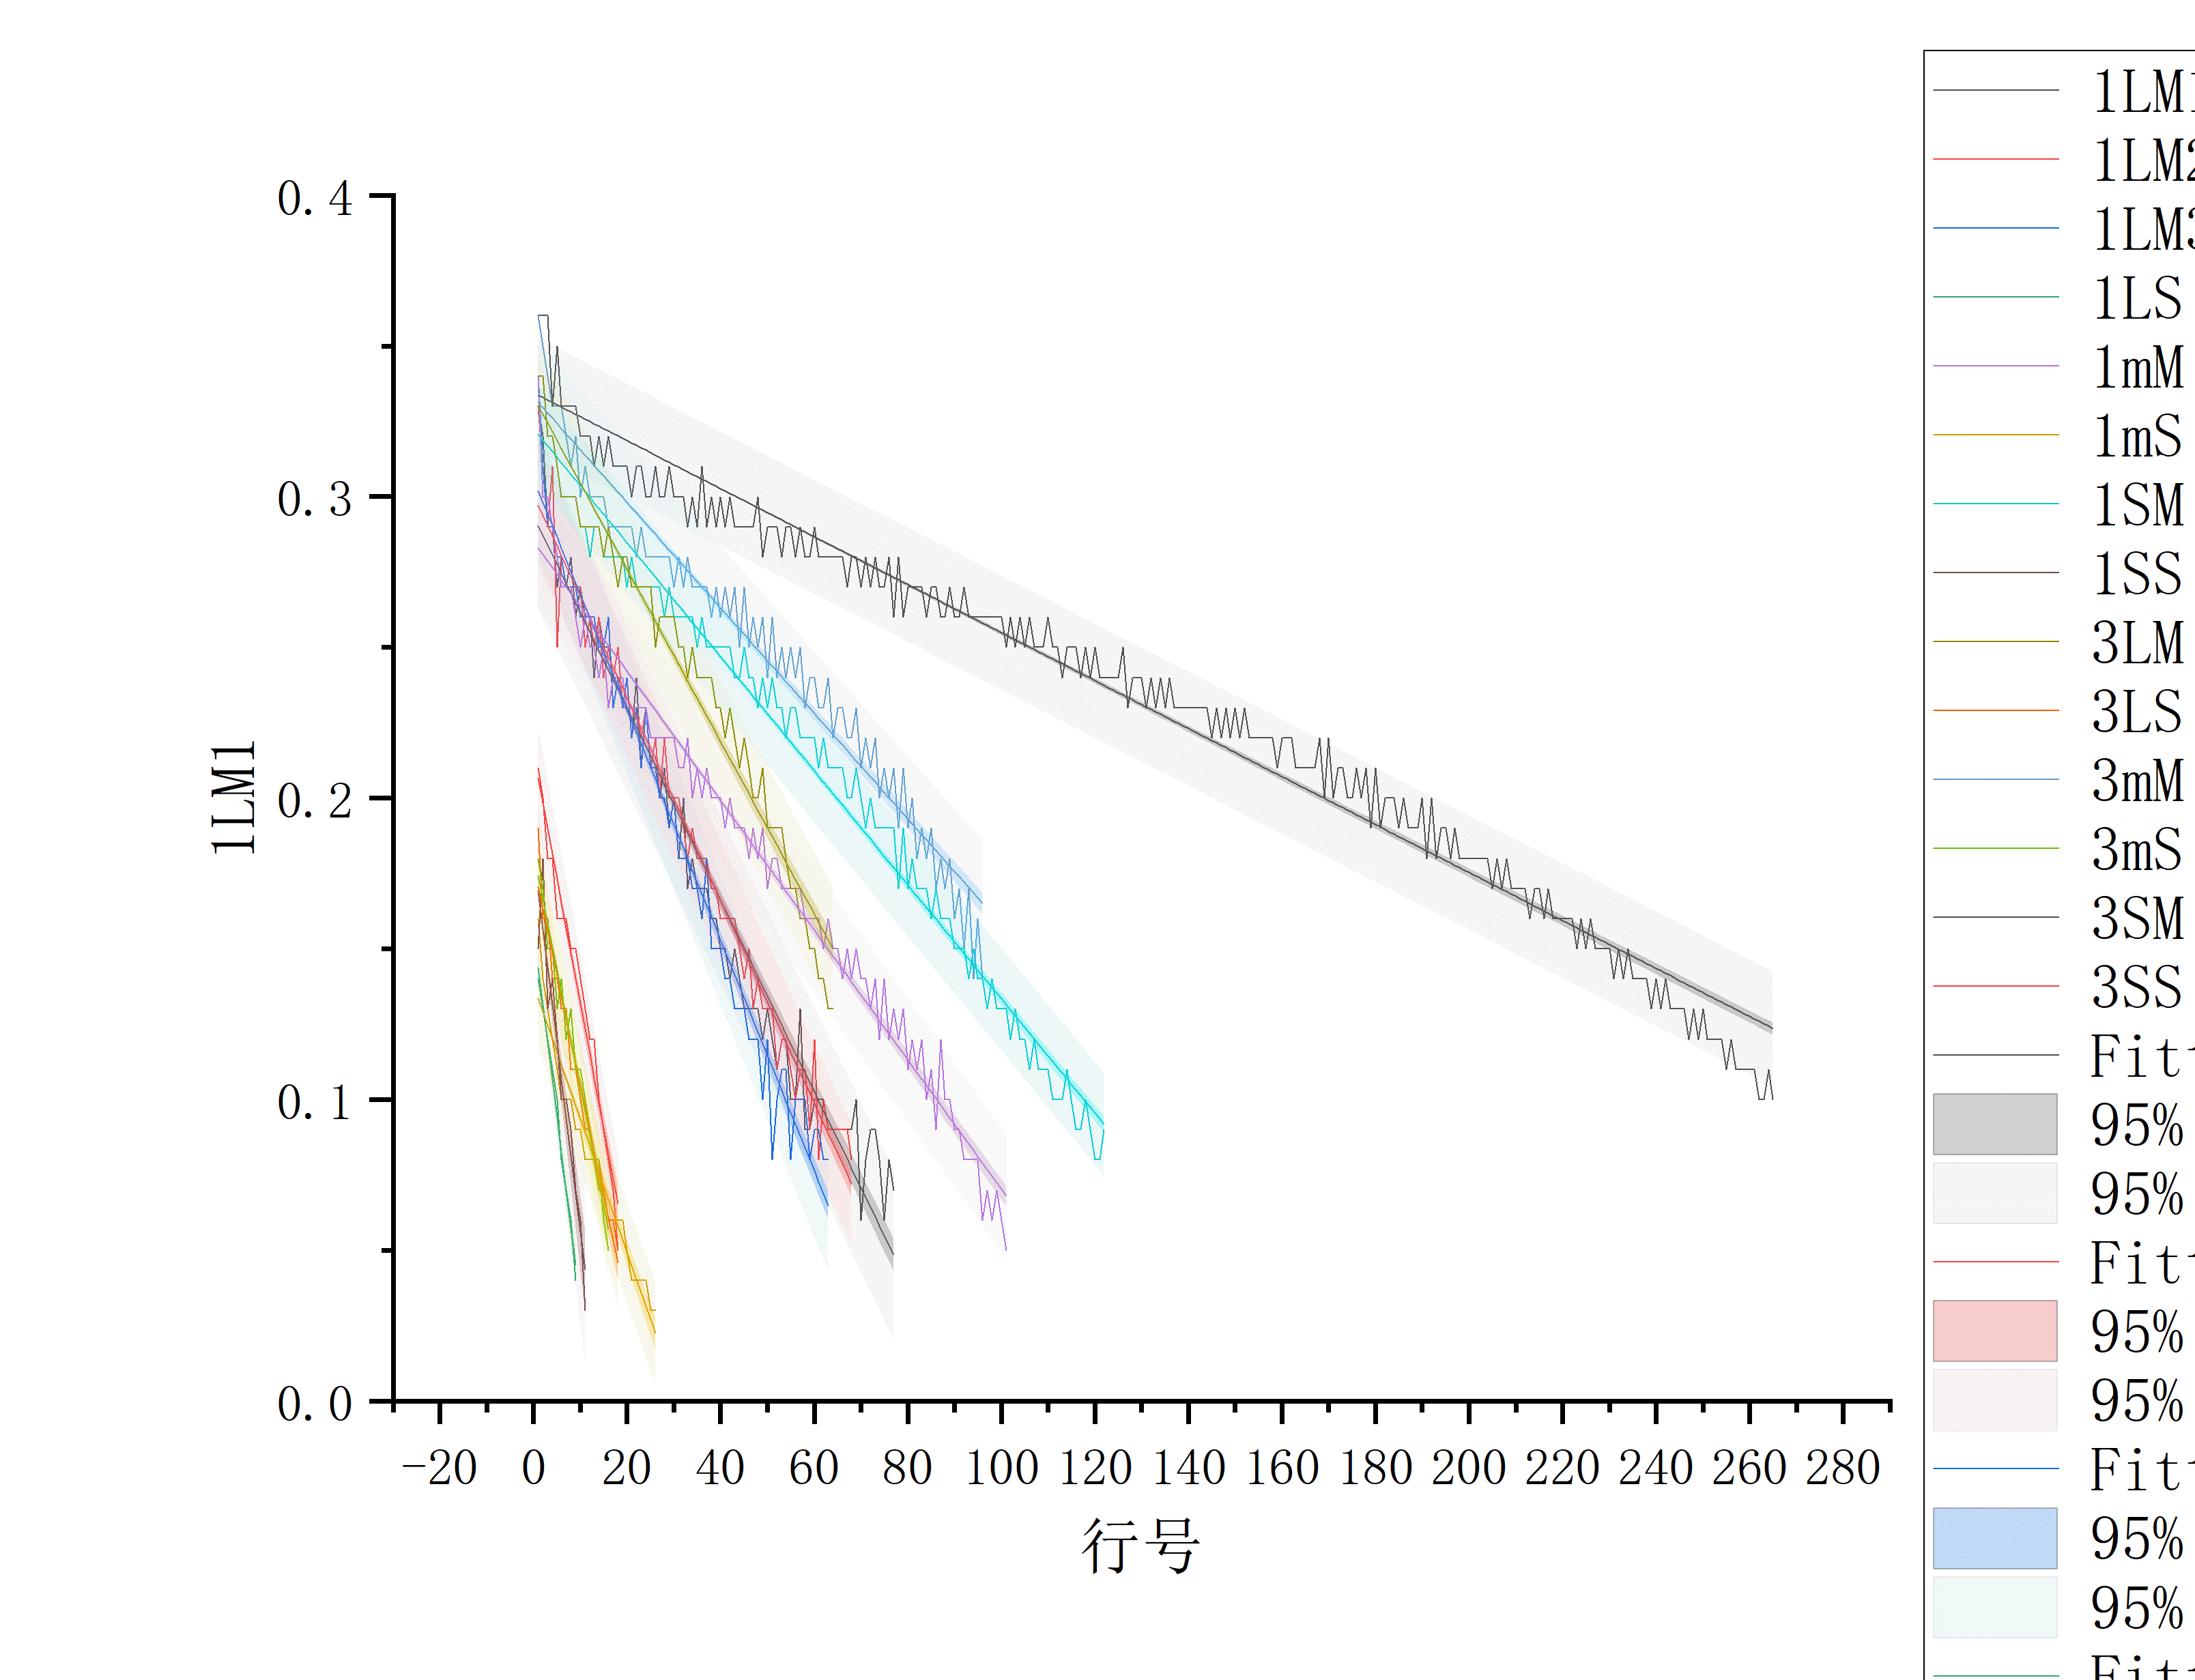
\includegraphics[width=0.4\textwidth]{figures/拟合次数1.png}
    }
    \subfloat[拟合次数2]{
        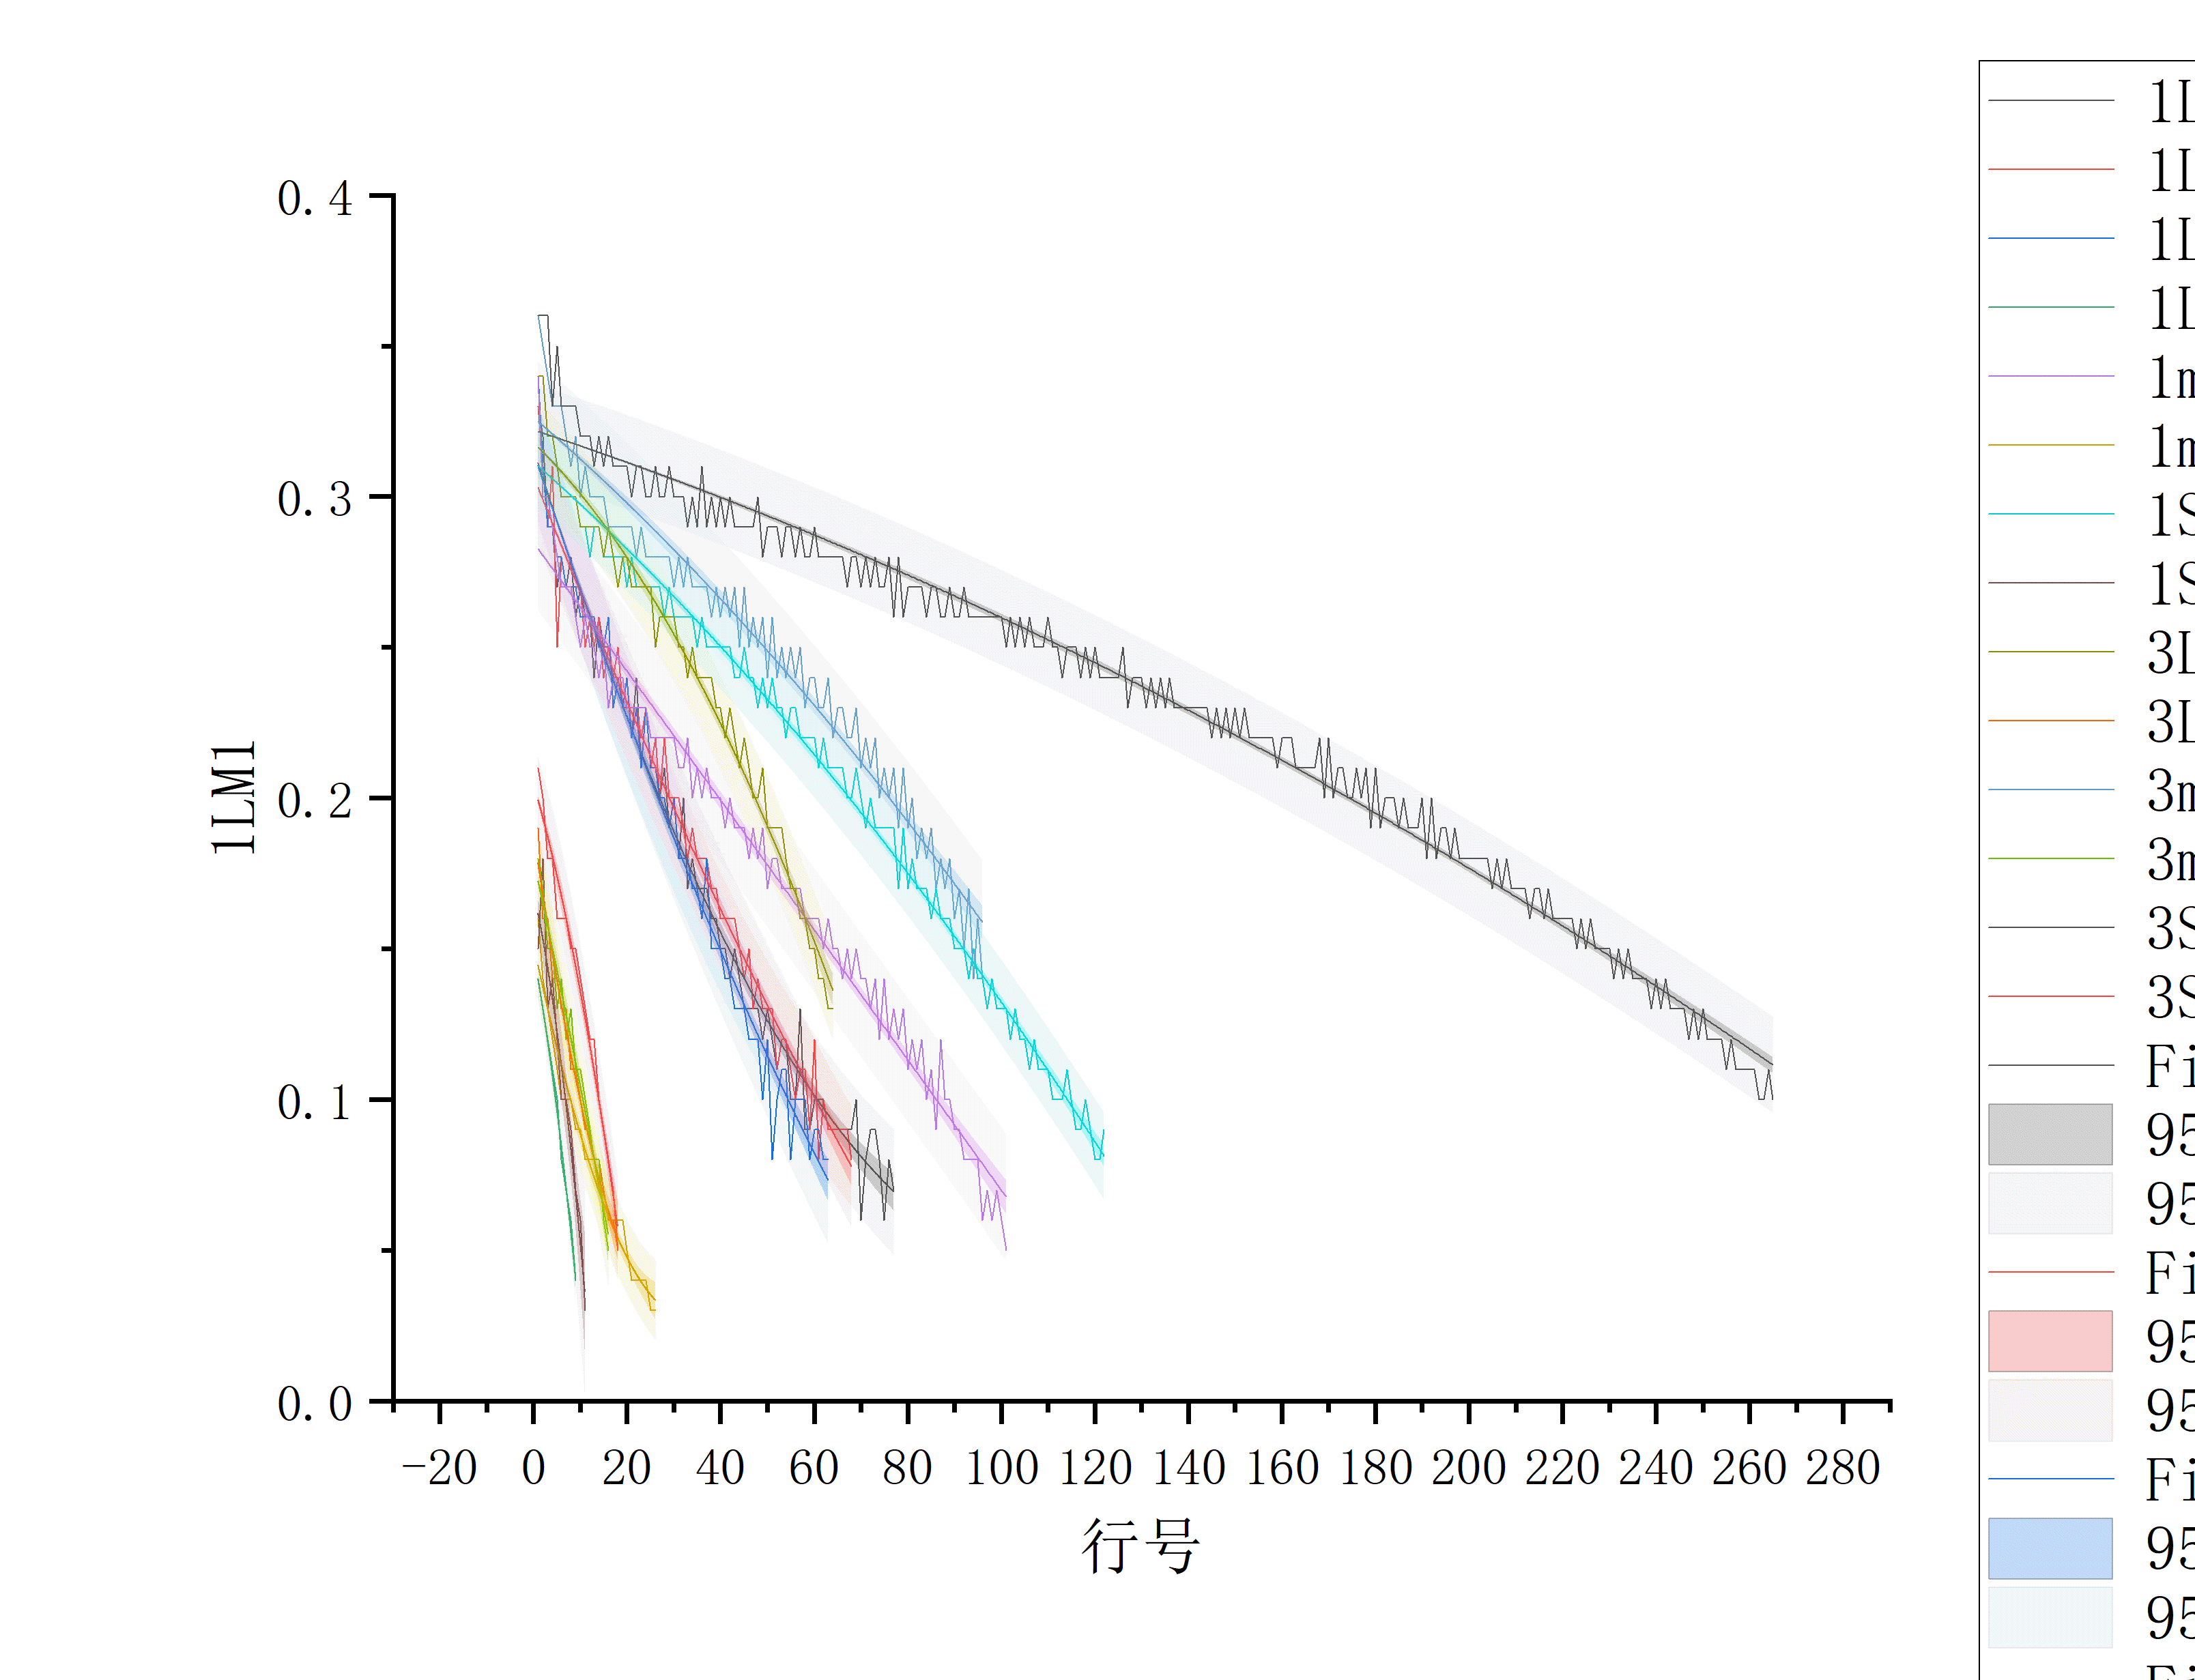
\includegraphics[width=0.4\textwidth]{figures/拟合次数2.png}
    }
    \caption{总体数据拟合}
    \label{总体数据拟合}
\end{figure}

\begin{figure}[H]
    \centering
    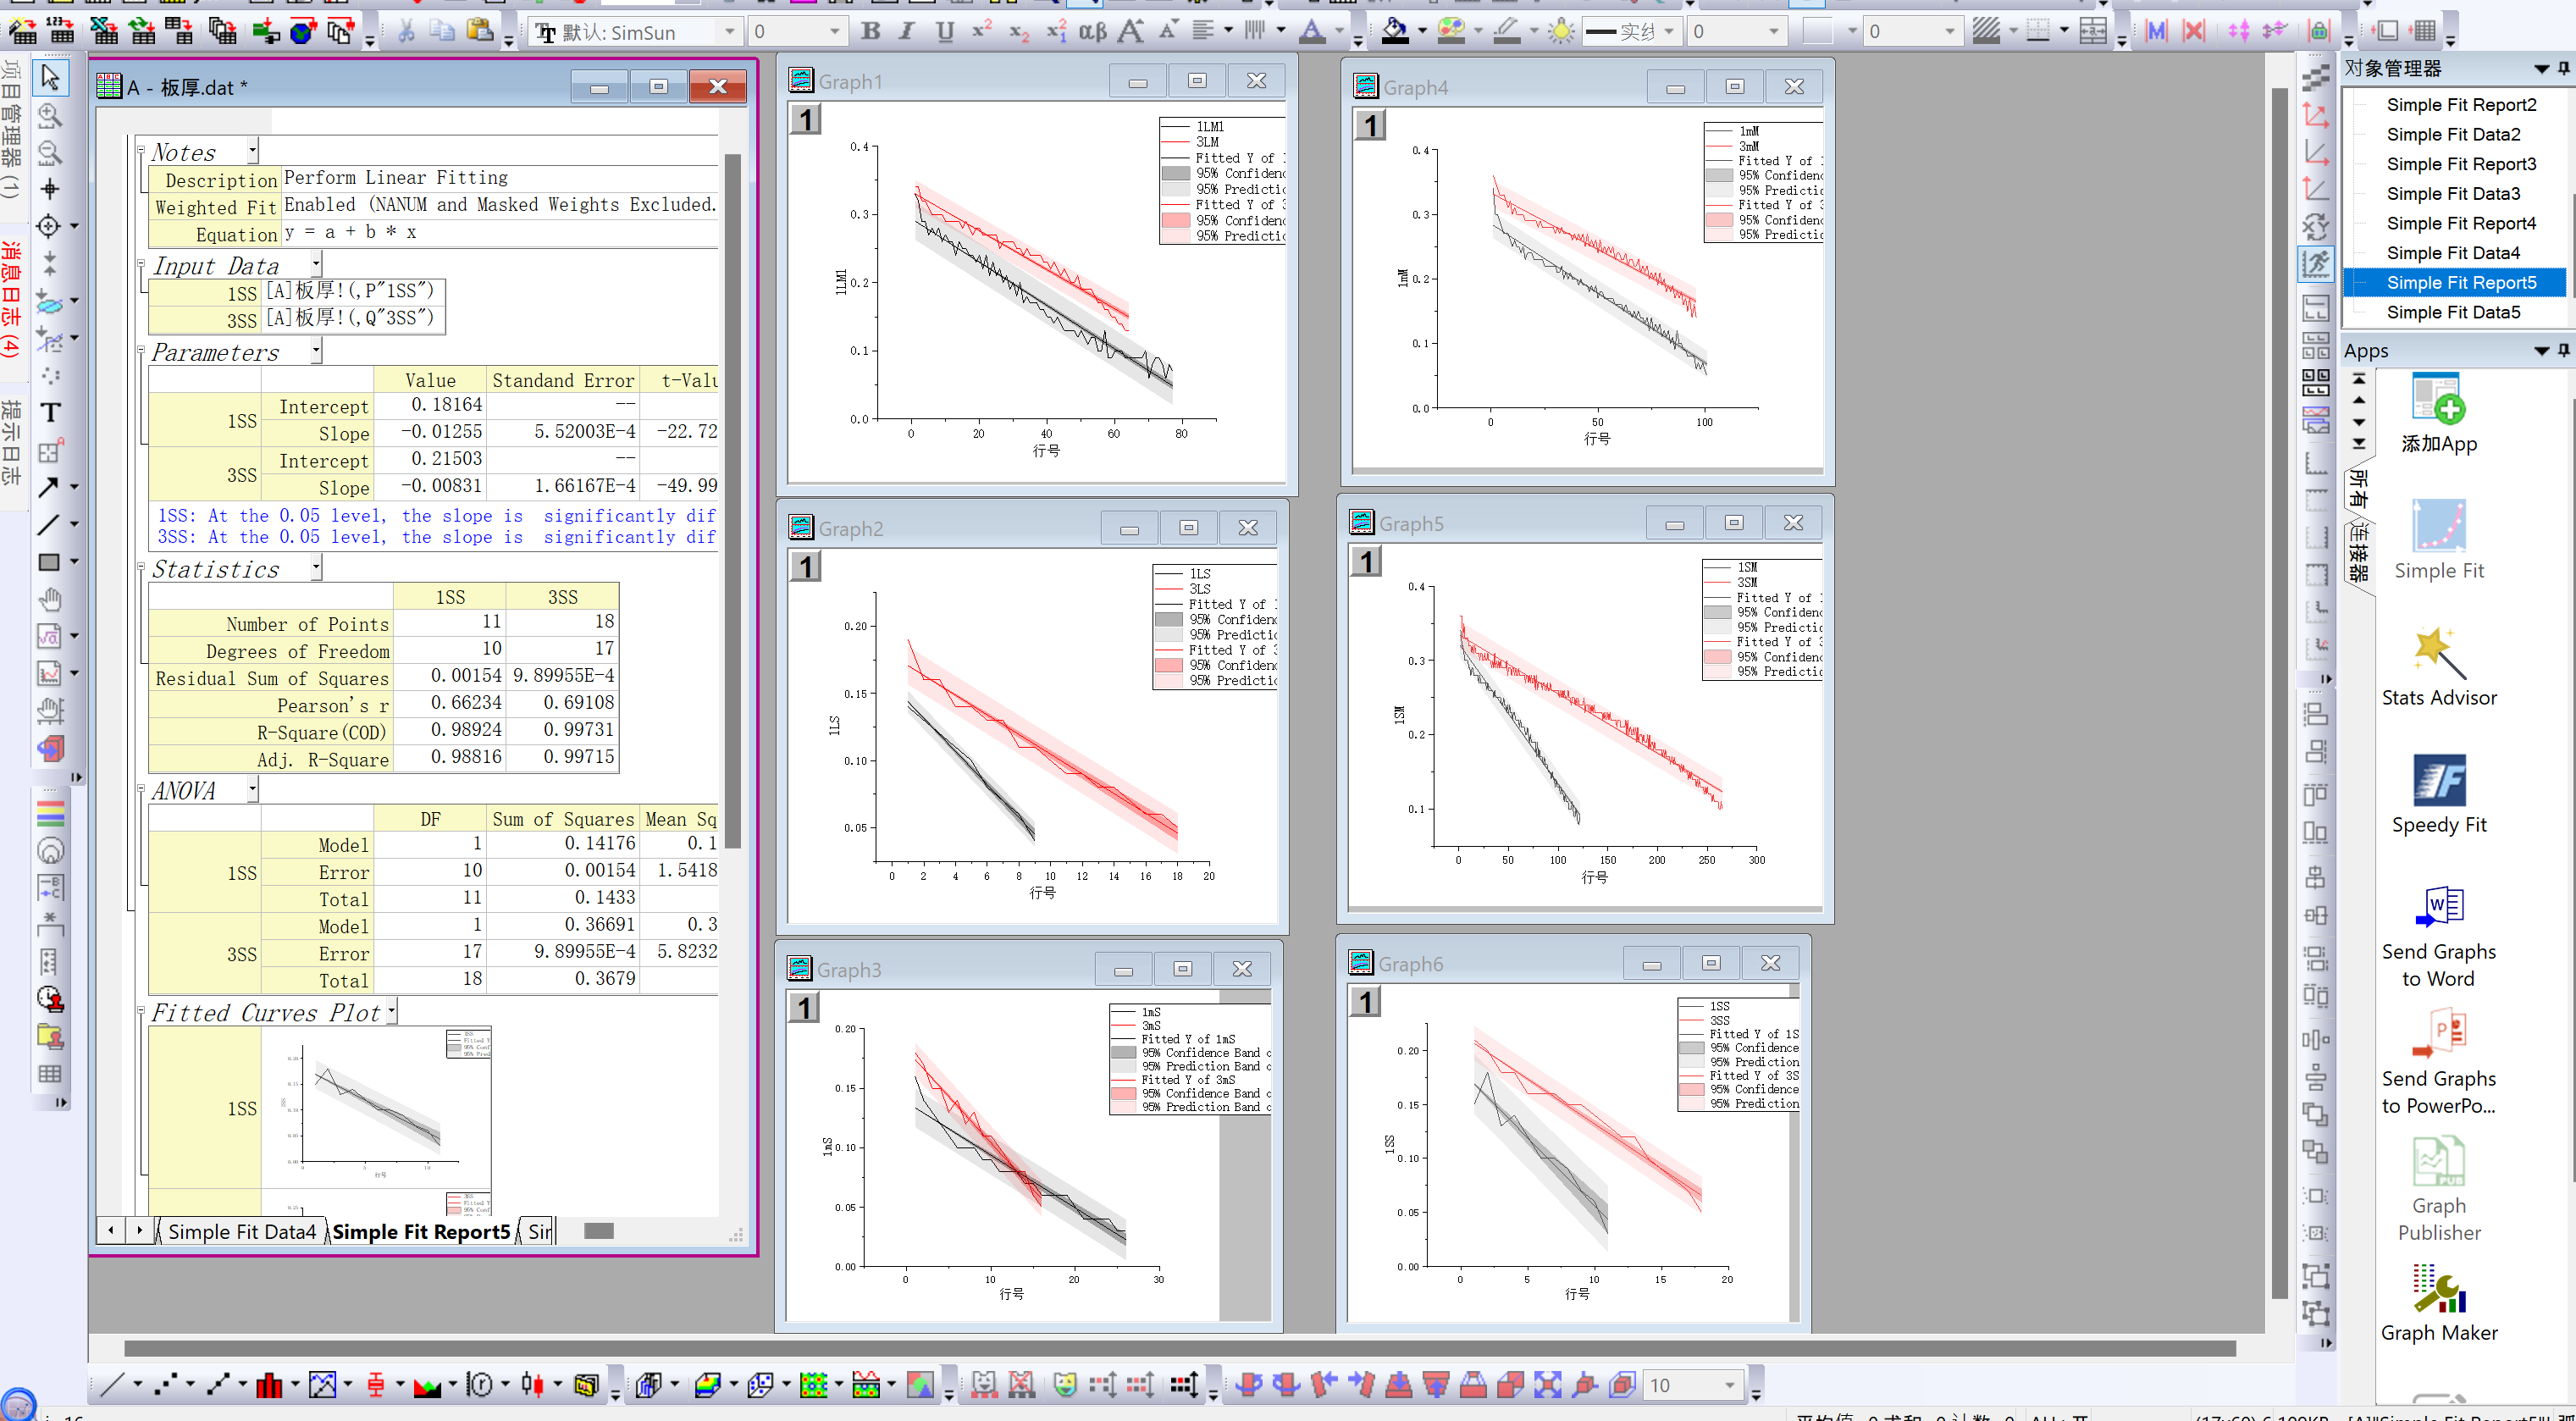
\includegraphics[width=10cm]{figures/板厚.png}
    \caption{改变介质板厚}
    \label{改变介质板厚}
\end{figure}

\begin{figure}[H]
    \centering
    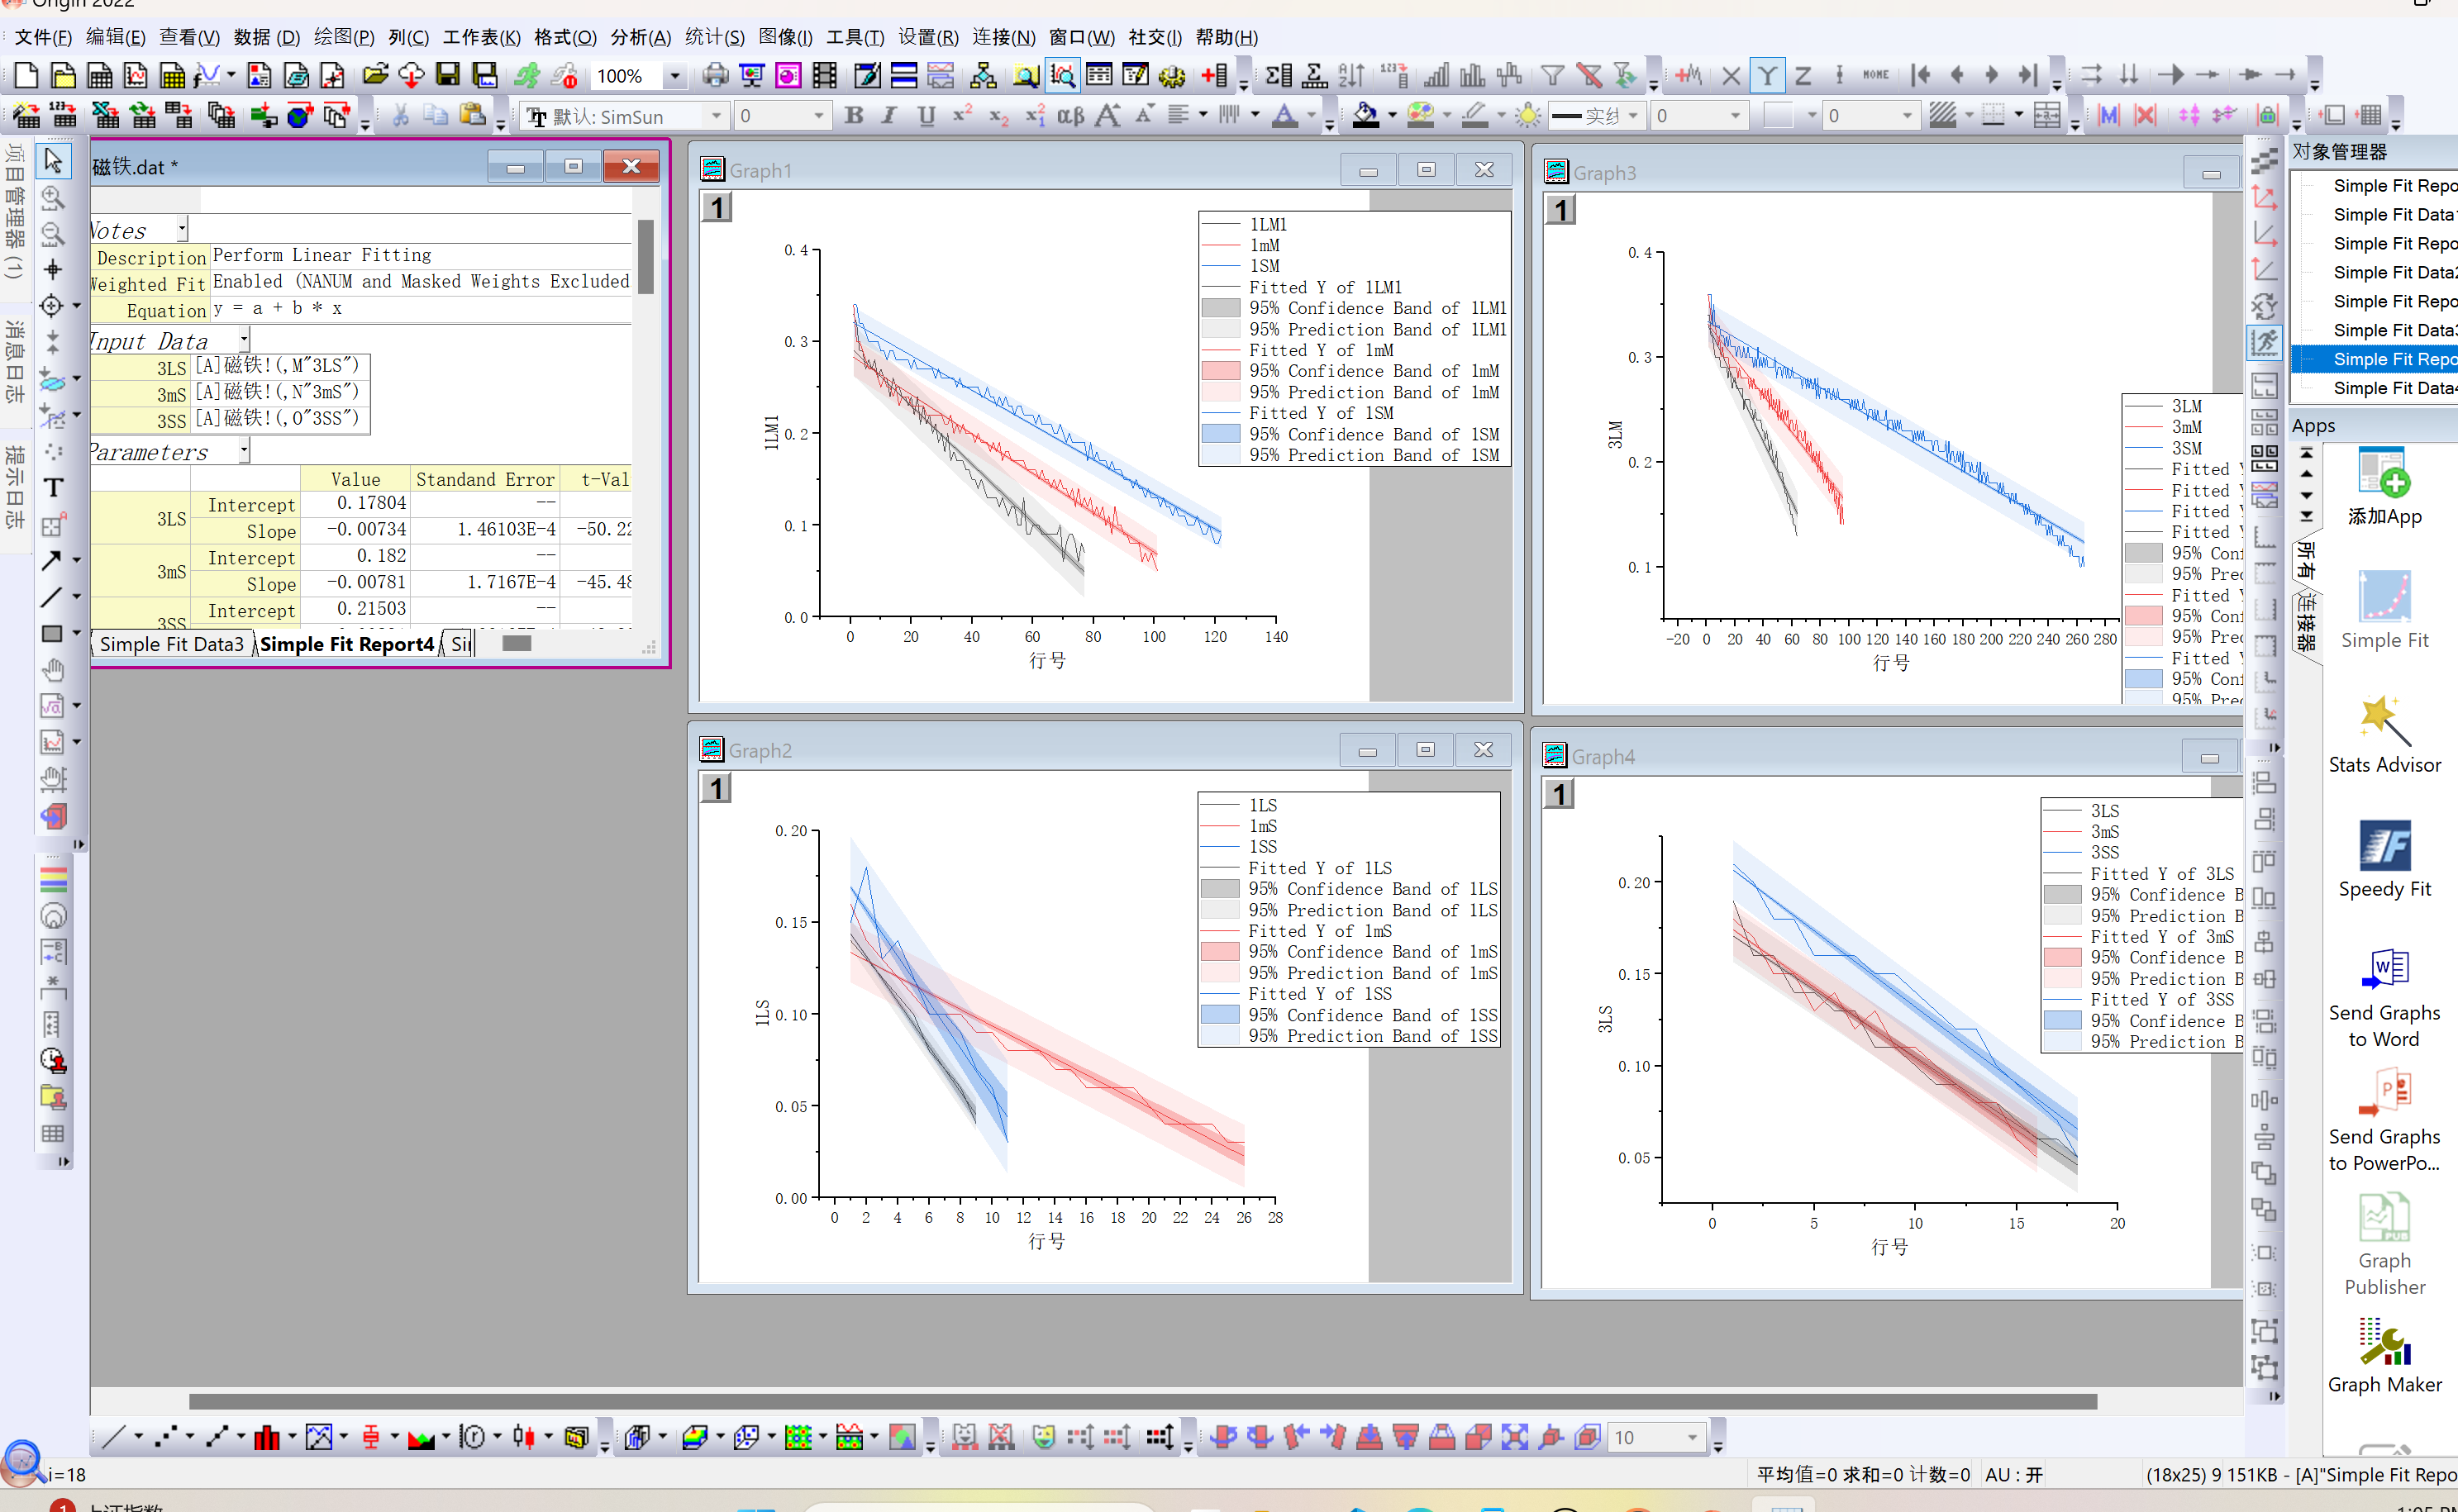
\includegraphics[width=10cm]{figures/磁场分布.png}
    \caption{改变磁场分布}
    \label{改变磁场分布}
\end{figure}

\begin{figure}[H]
    \centering
    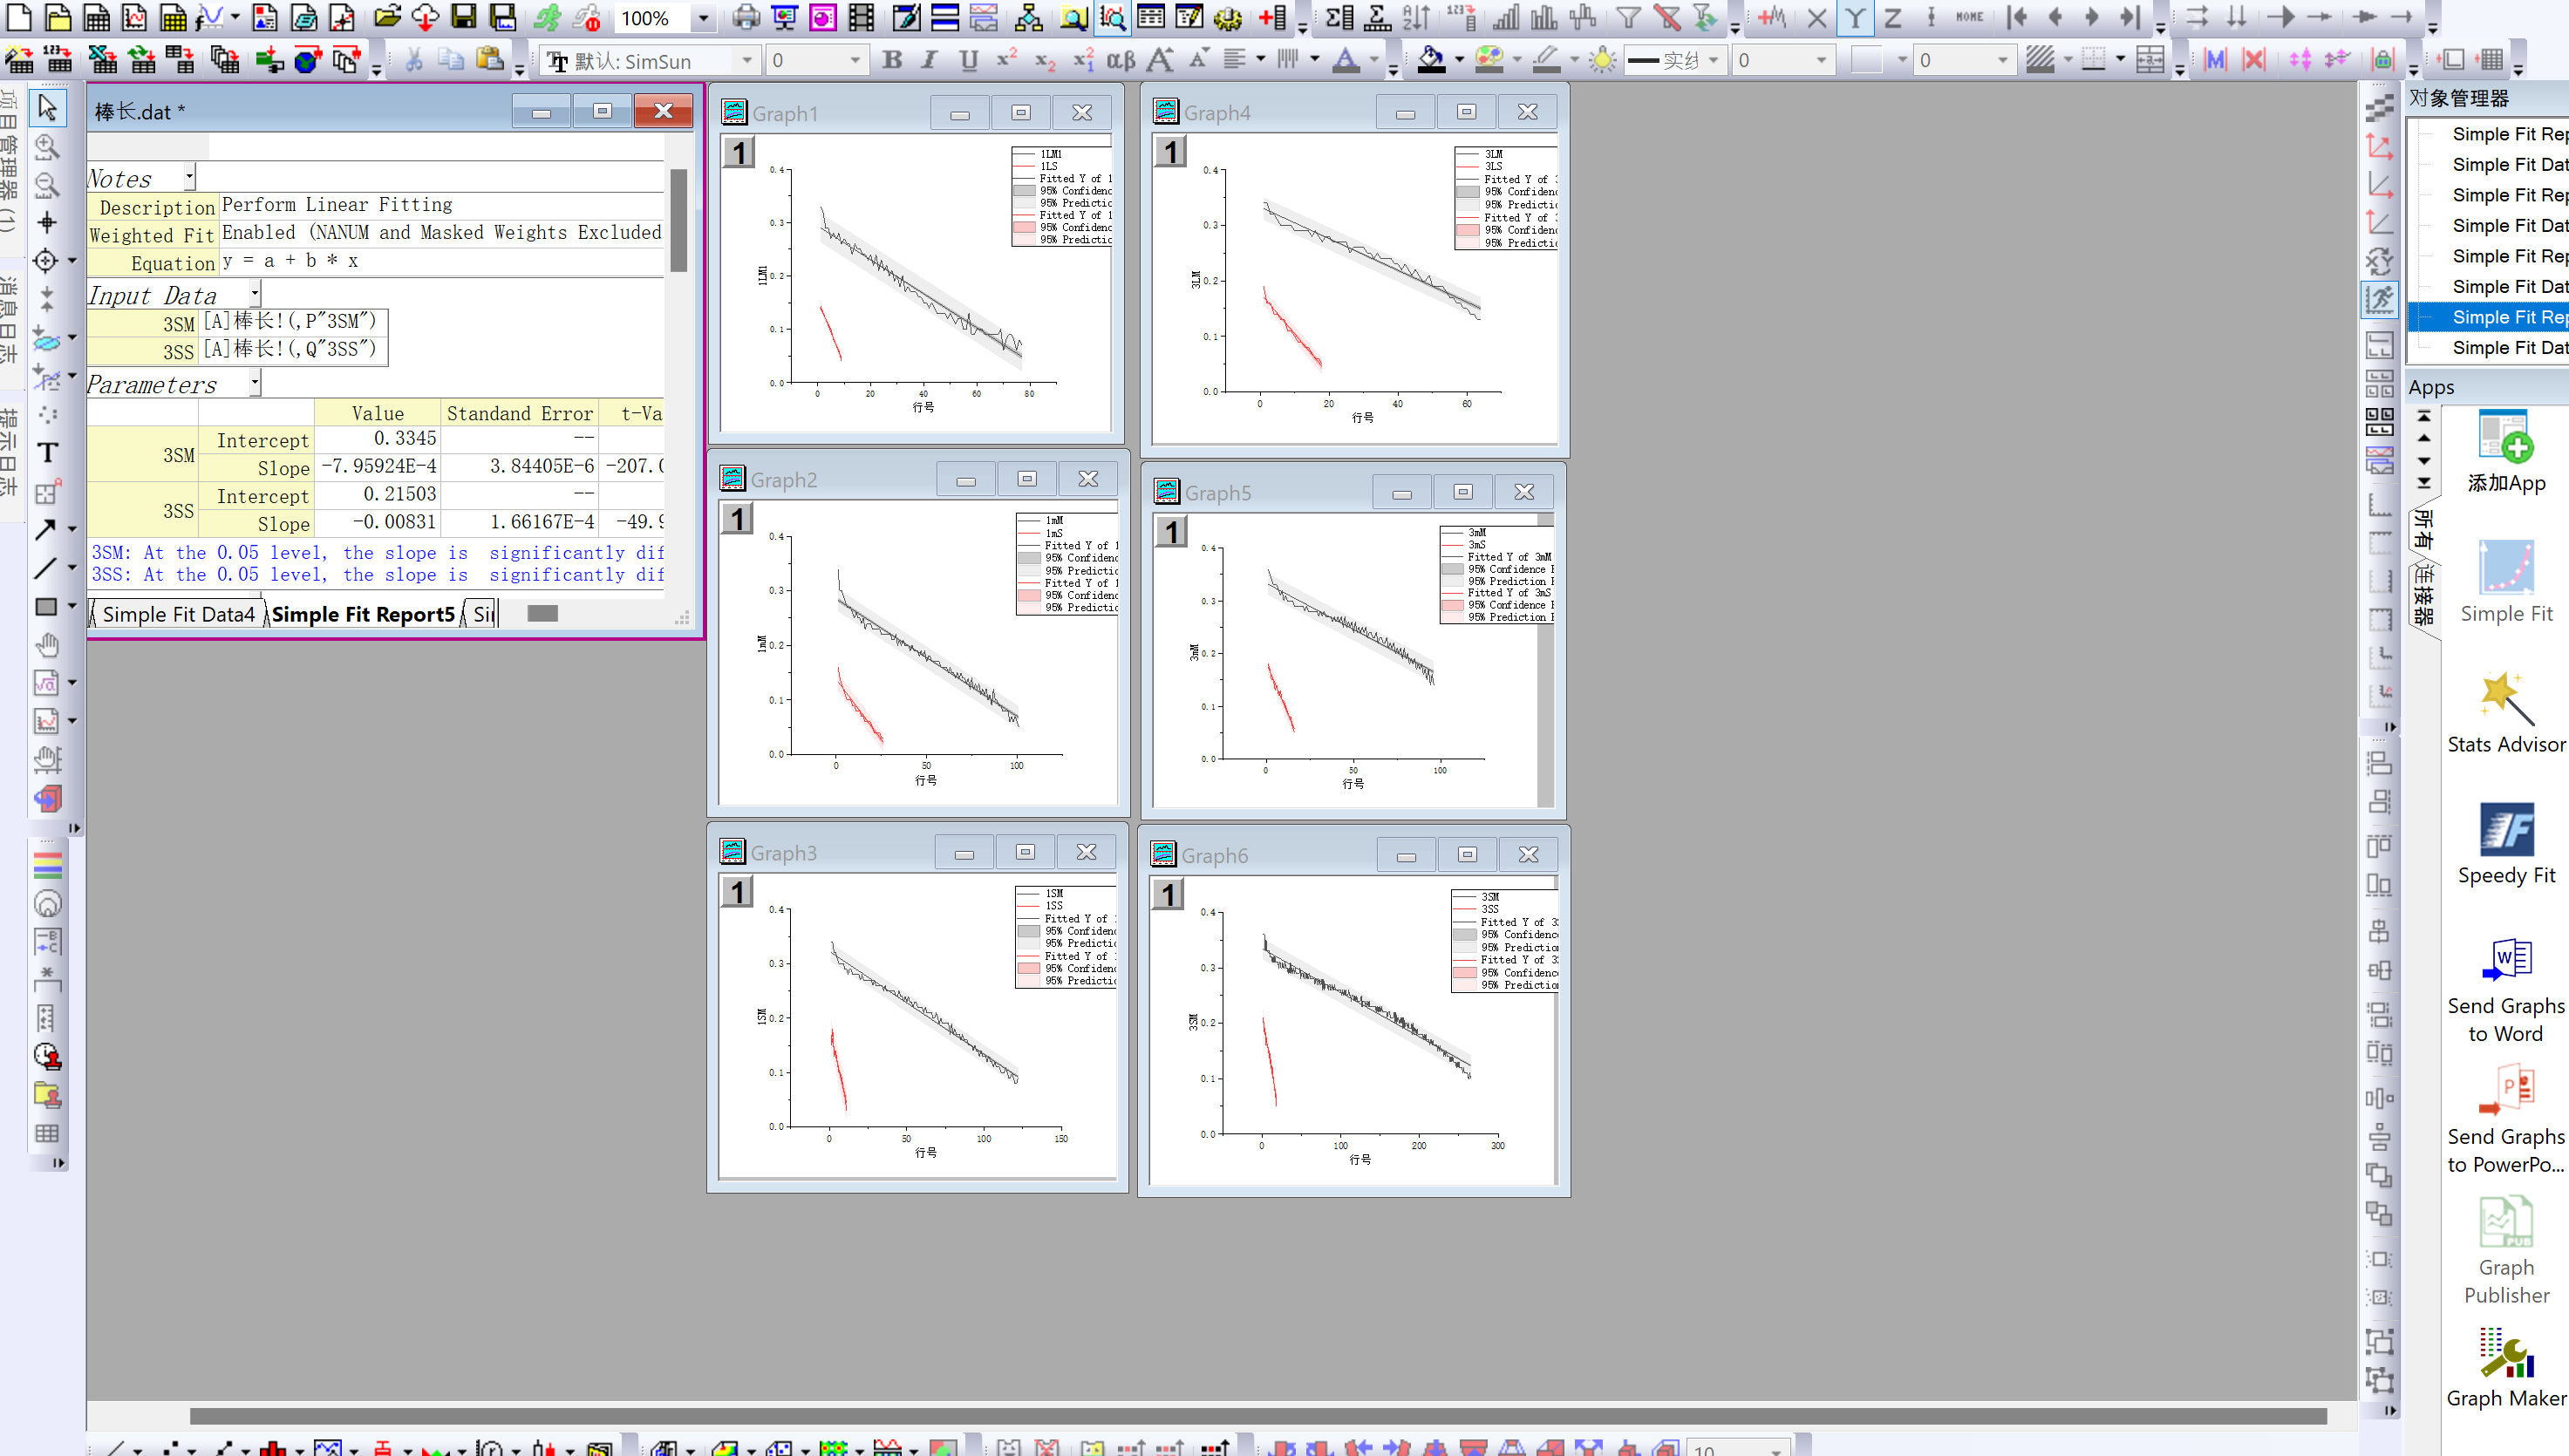
\includegraphics[width=10cm]{figures/棒长.png}
    \caption{改变磁棒长度}
    \label{改变磁棒长度}
\end{figure}
如图\ref{改变介质板厚}、\ref{改变磁场分布}、\ref{改变磁棒长度}分别给出控制介质板
厚度、磁场分布、棒长的结果,从对比之中我们可以得到一下结果:
\begin{itemize}
    \item 介质板越厚,相同倾角,摆动的周期越大;且周期衰减的越慢;
    \item 磁铁对磁棒的影响比较复杂,现有的数据无法做出较为严谨的判断;
    \item 棒越长,周期越大,周期衰减越慢。
\end{itemize}


\chapter{数值计算与仿真模拟}
\section{数值计算}
项目通过尝试Monte Carlo 算法、Adaptive complex Simpson 算法、
Gauss 积分、Romberg积分等\cite{Numerical_Analysis}。综合考虑效率、精确度等,可行性最高的是Romberg积分。
但是个人电脑的算力只能给出小数点后4-5位的磁场精度,精度达不到计算磁棒受力的要求。
但通过数值计算,可以解决上述问题之一——介质板只有在厚度不是太小时,才能使轴线成为
一个稳定的平衡点。

如图\ref{zmag}和\ref{z24},随着z的增大,轴逐渐成为磁场的极大值点。
\begin{figure}[H]
    \centering
    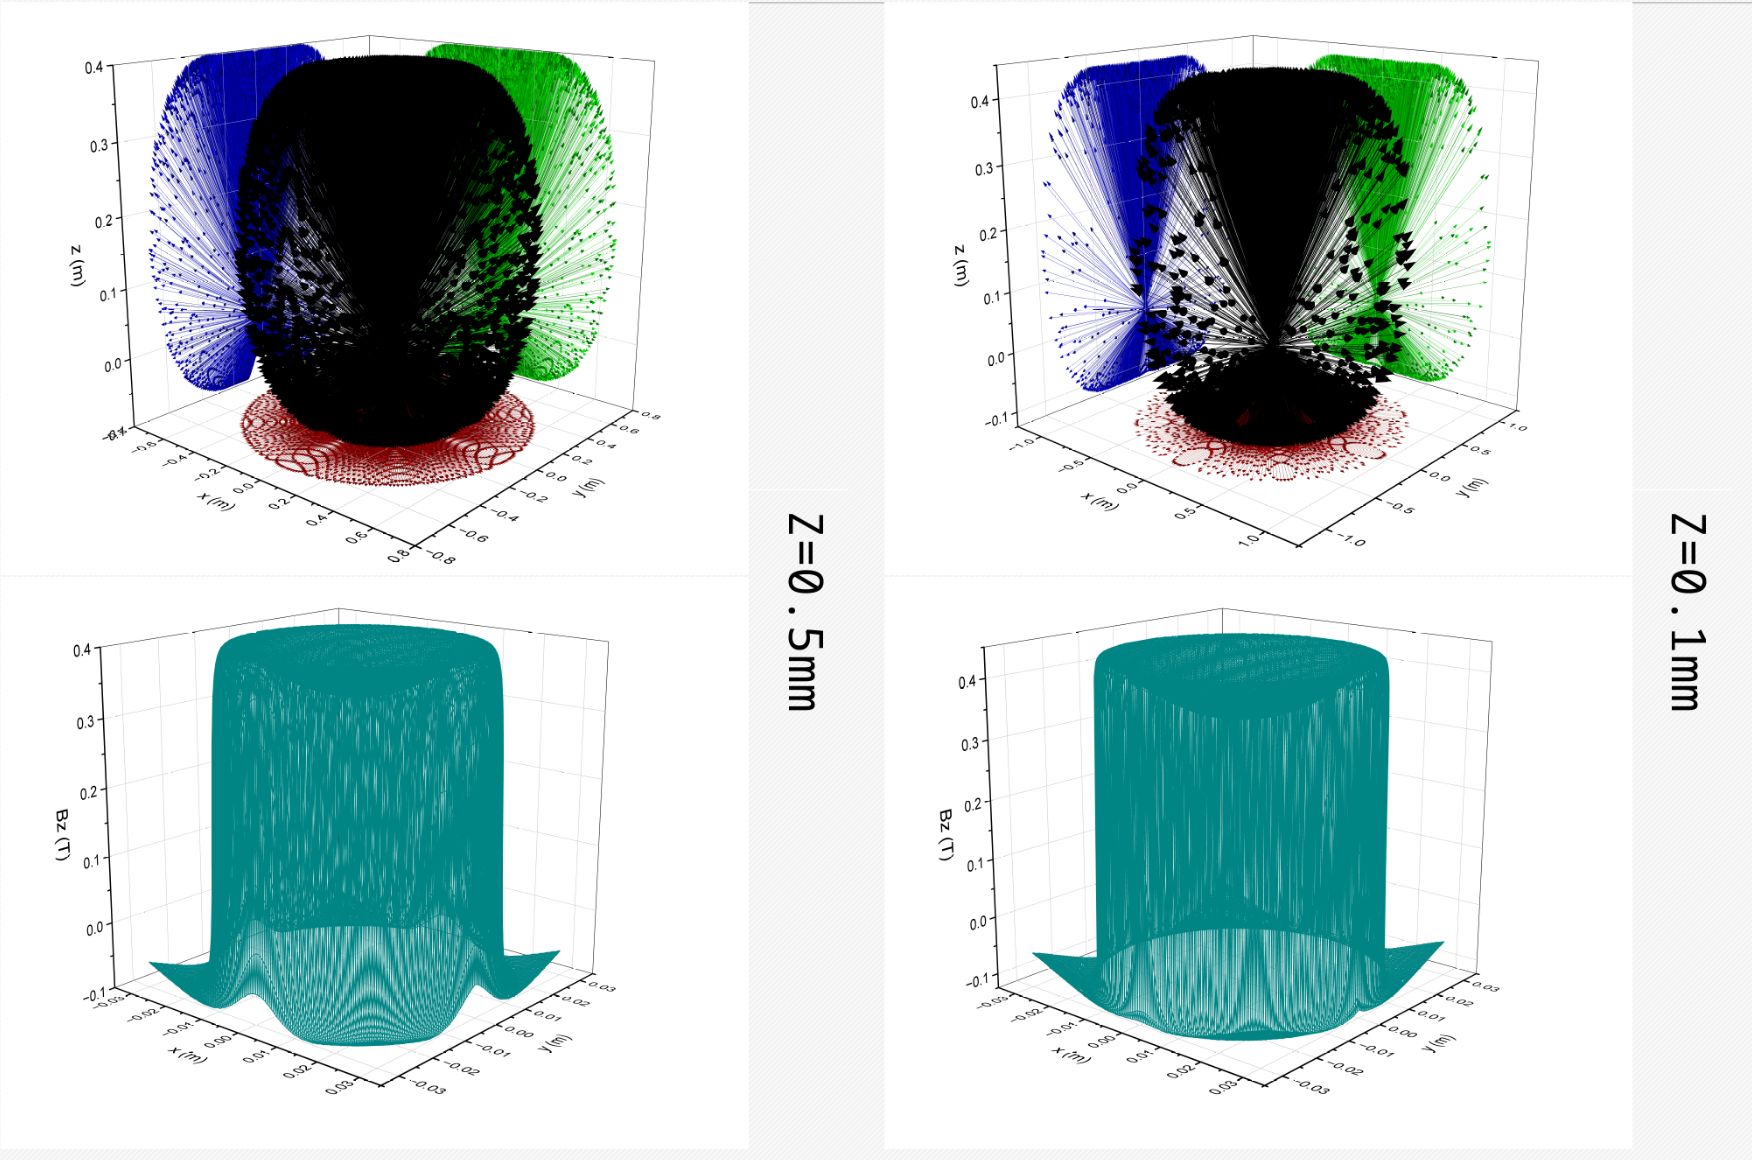
\includegraphics[width=12cm]{figures/Zmag.png}
    \caption{Z-magneticfield}
    \label{zmag}
\end{figure}

\begin{figure}[H]
    \centering
    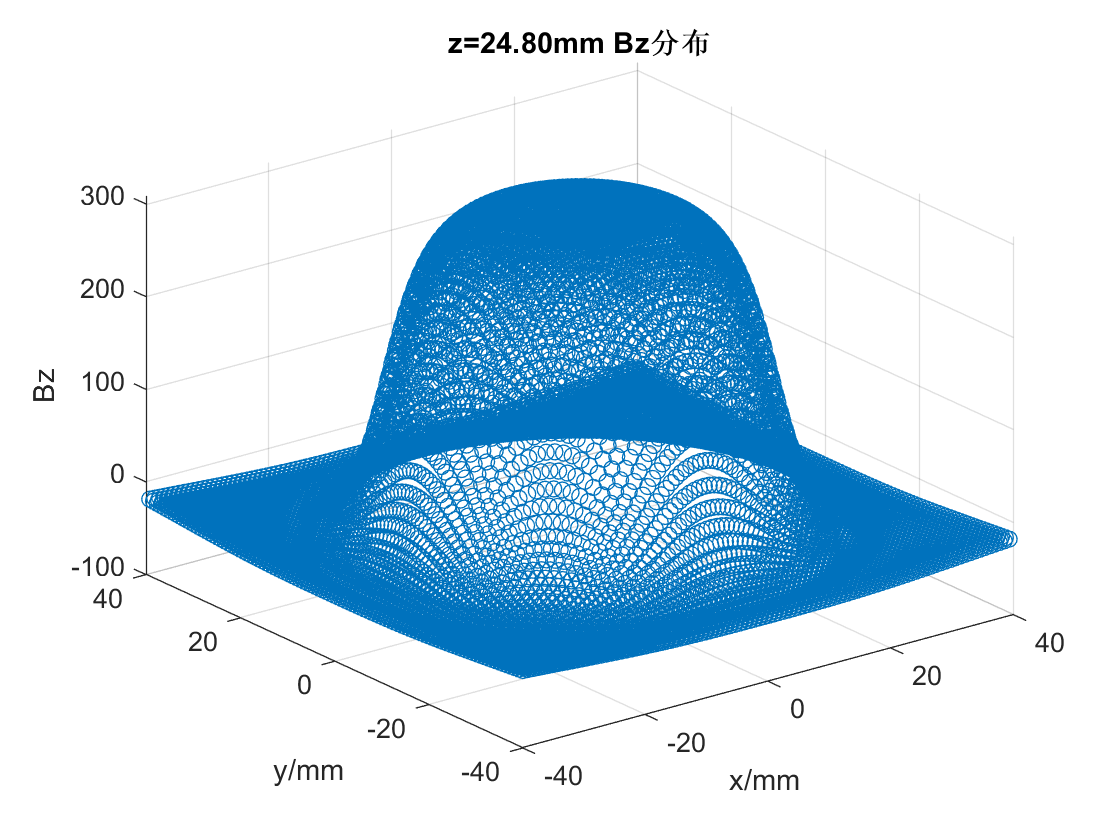
\includegraphics[width=8cm]{figures/z24.png}
    \caption{Z-24}
    \label{z24}
\end{figure}

\section{COMSOL 模拟}
通过COMSOL模拟物理场(图\ref{COMSOL}),可以得到棒长与周期的定性关系——周期
随棒长增大而增加(如图\ref{COMSOL结果})。同时在棒长较短时,仿真与实验拟合
较好。可能的原因是当棒长较长时,棒与介质板接触不仅密导致的。

但是板厚的变化对周期的影响模拟结果并没有体现。


\begin{figure}[H]
    \centering
    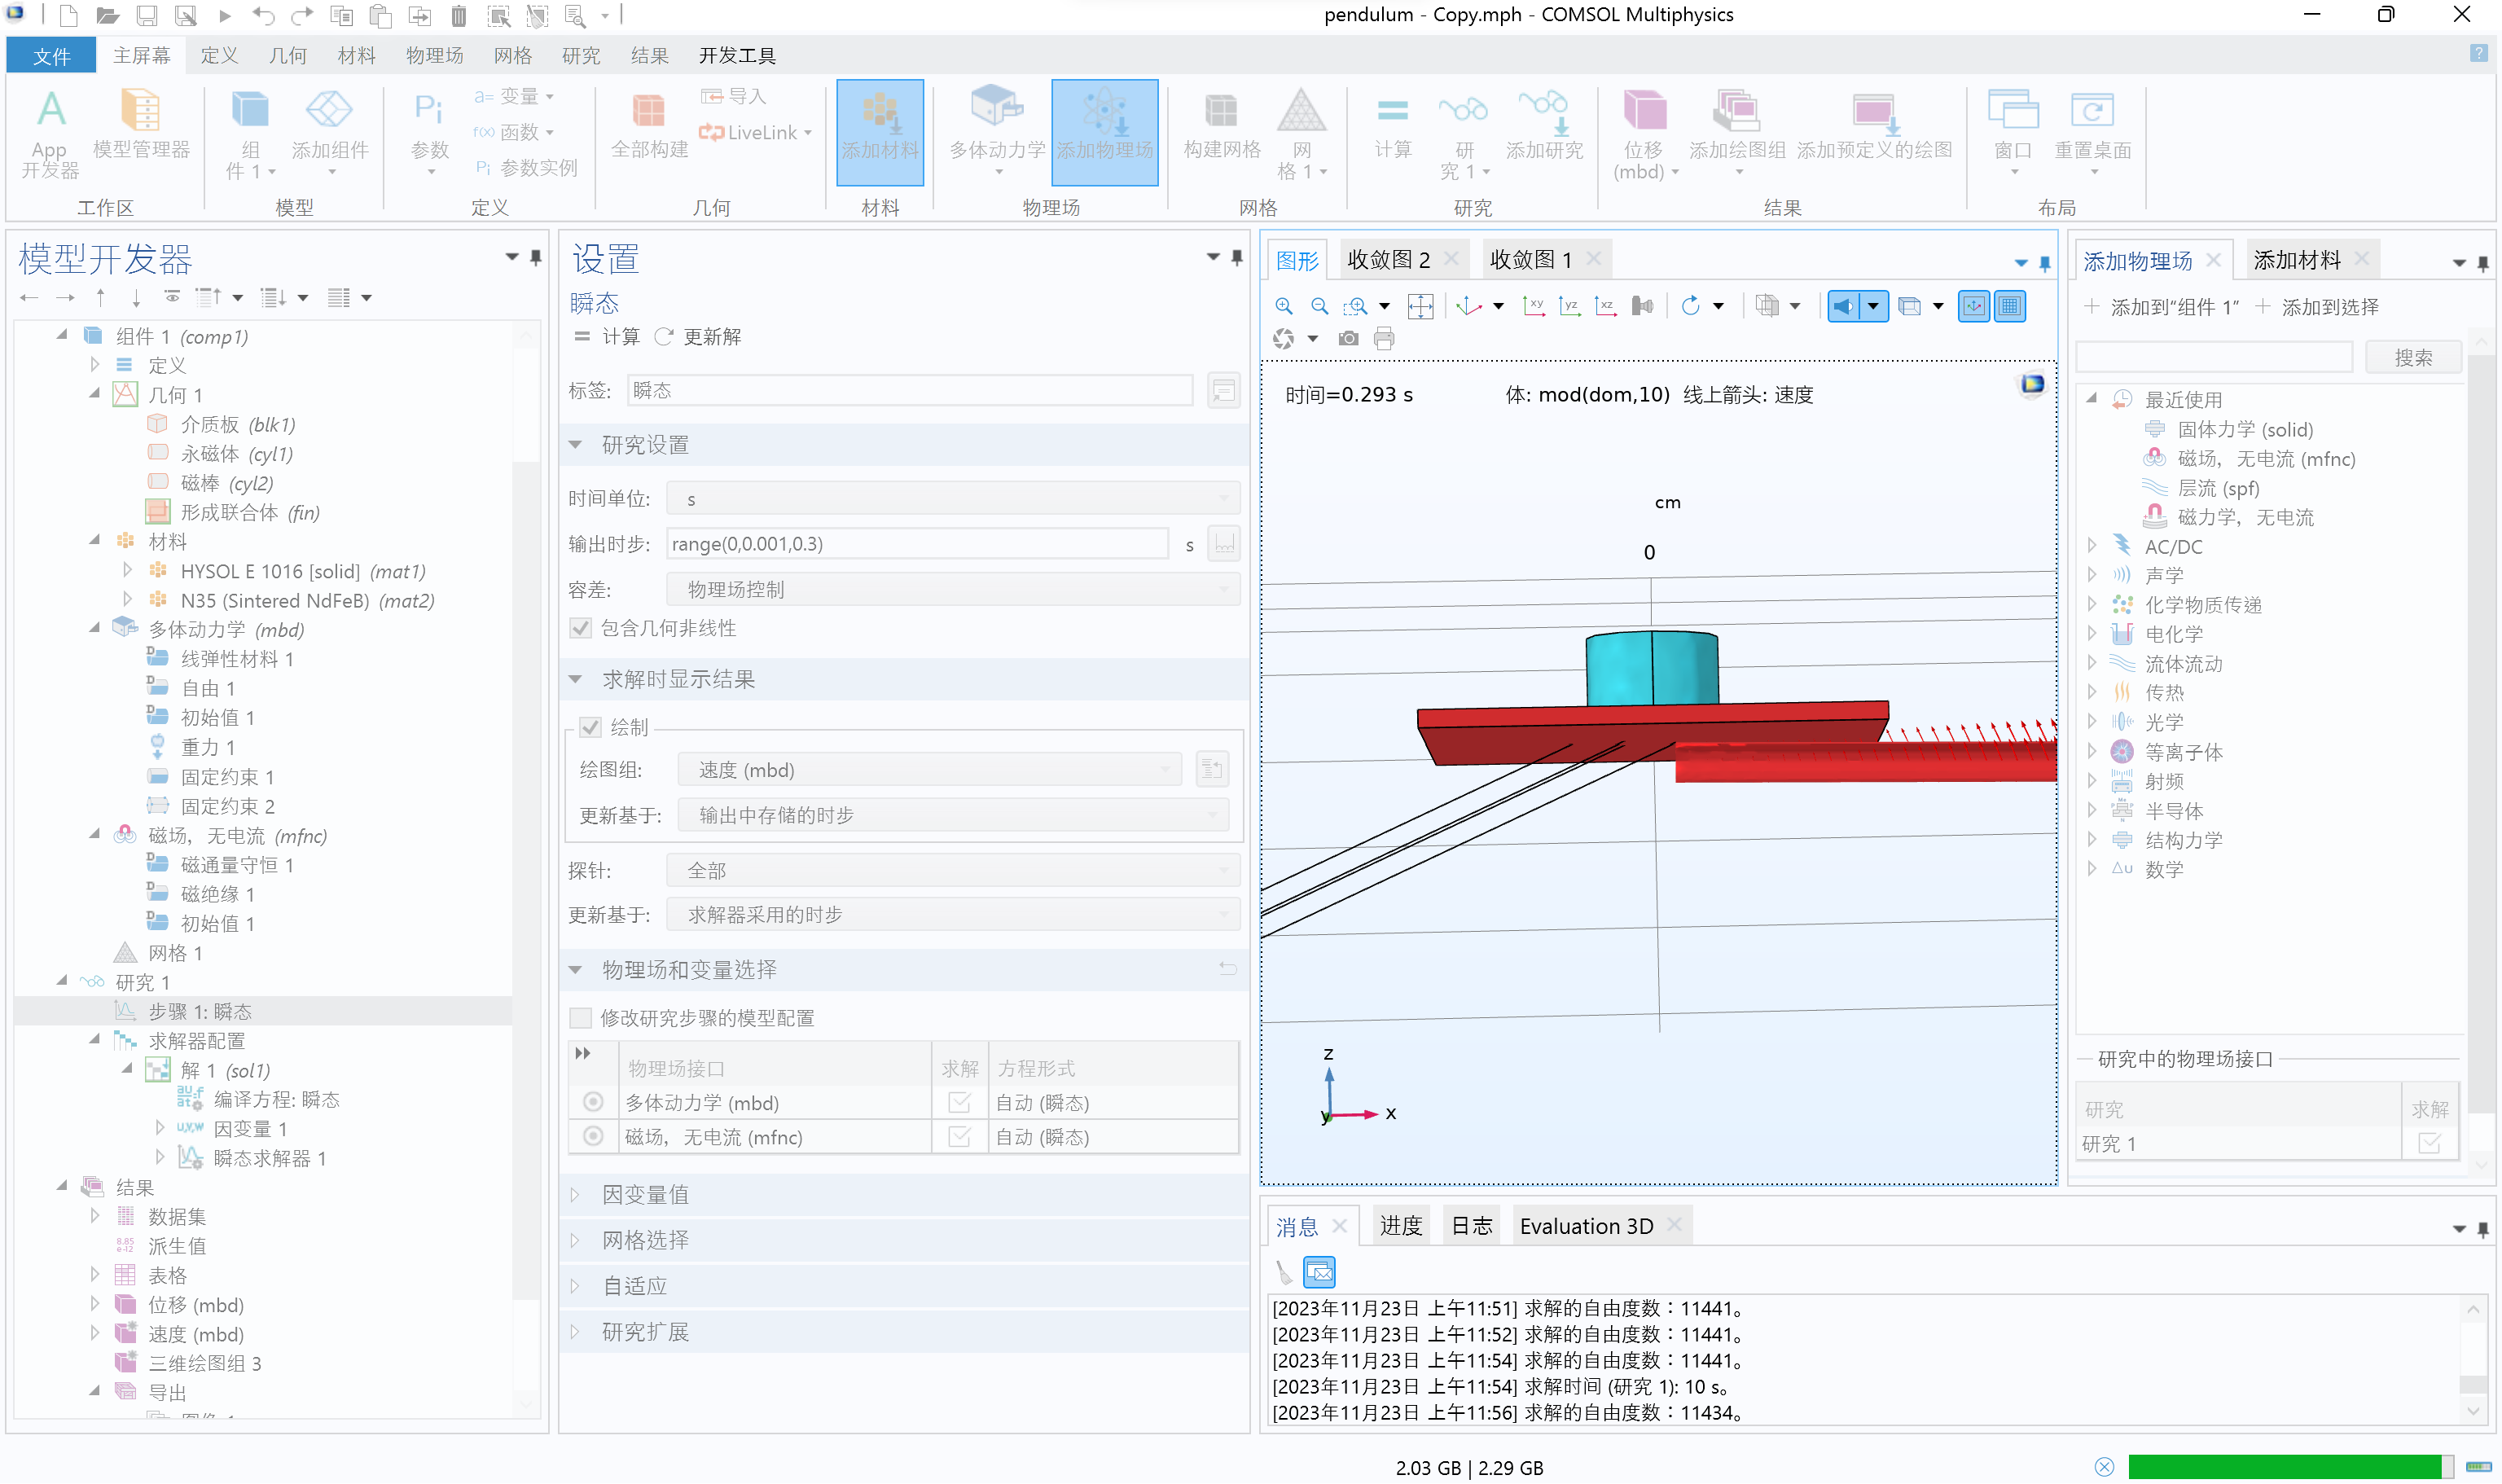
\includegraphics[width=12cm]{figures/COMSOL.png}
    \caption{COMSOL模拟}
    \label{COMSOL}
\end{figure}


\begin{figure}[H]
    \centering
    \subfloat[模拟1]{
        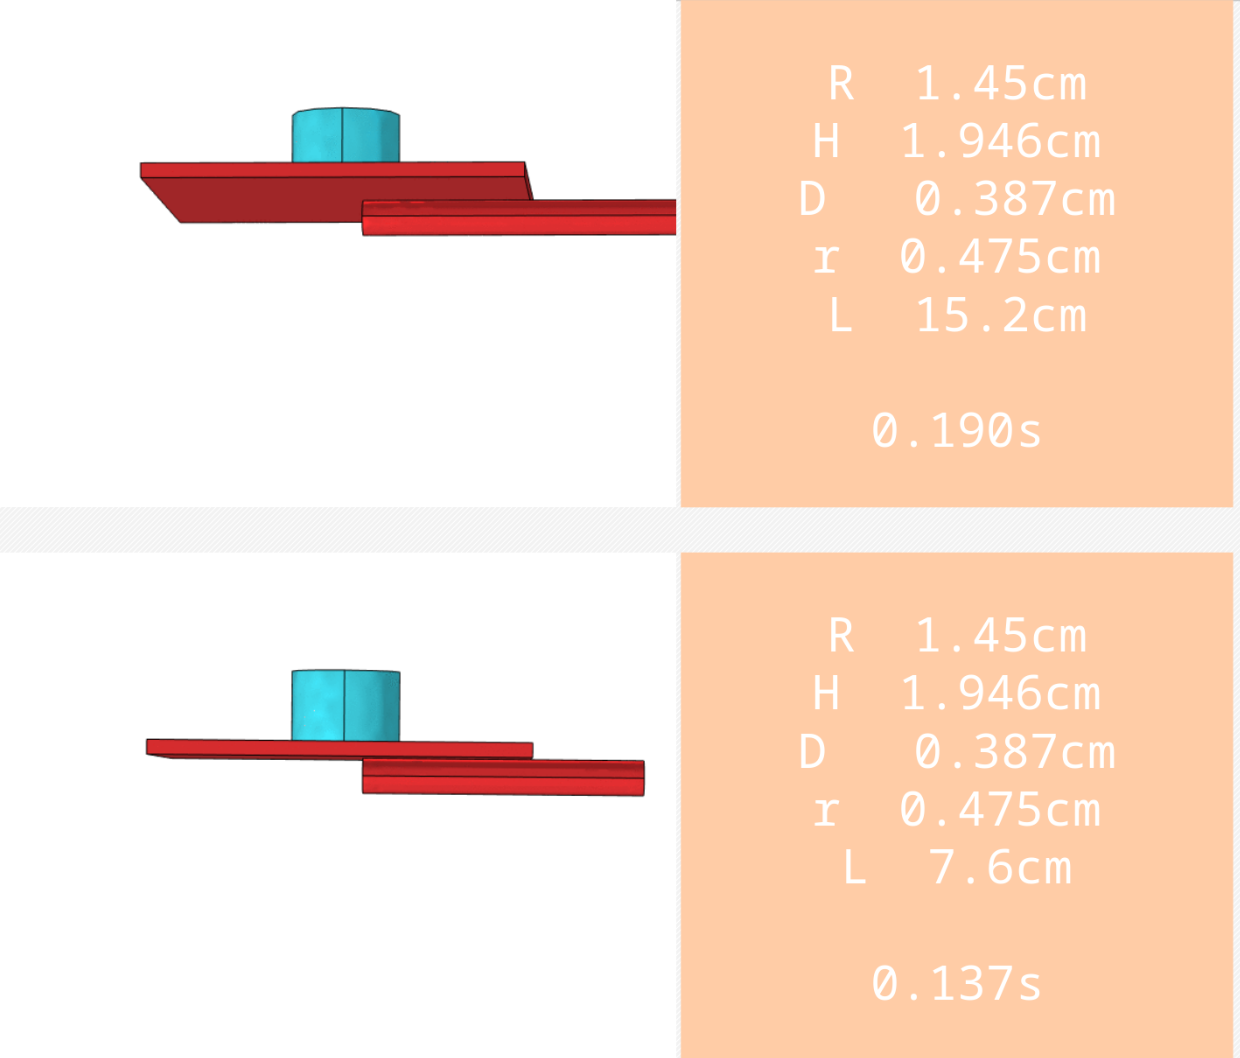
\includegraphics[width=0.4\textwidth]{figures/387.png}
    }
    \subfloat[模拟2]{
        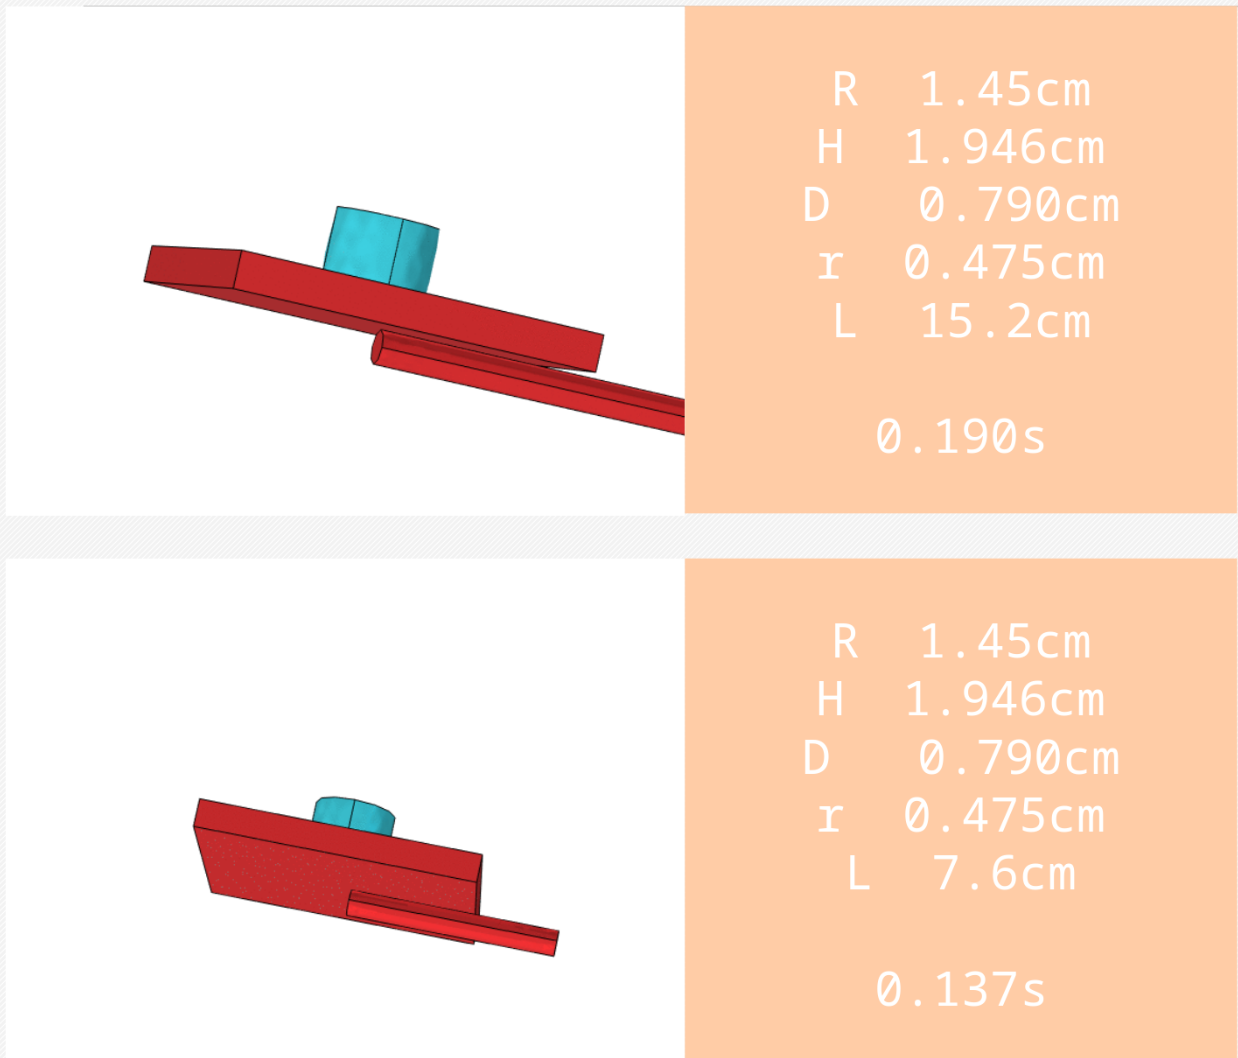
\includegraphics[width=0.4\textwidth]{figures/790.png}
    }
    \caption{COMSOL模拟结果}
    \label{COMSOL结果}
\end{figure}

\chapter{总结与展望}
研究利用多种方法对欧拉摆这个复杂的物理
体系进行分析,得到了许多有用的结果。但由于实
验器材、个人计算机算力等问题,得到的结果都十
分粗糙,理论得不到完备的检验,模拟结果与实验
的不符也难以进一步分析、验证。总体来说有以下
几个主要问题:

1.算力不够导致磁场的数值解只能精确 mT 的
量级,无法满足力场计算的要求,因此数值上无法
对周期进行求解。

2.对 COMSOL 并不熟练,导致出现了接触点处
贯穿的现象。

3.数值算法本身近似的缺点导致磁场本有的对
称性破坏,对结果造成很难预测的结果。

4.数值算法难以处理奇点问题,毕奥-萨法尔定
律的缺陷在数值计算中是存在的,即电流元模型在
距离很近时是不成立的。

期待进一步的研究解决它们。
%论文后部
\backmatter


%=======%
%引入参考文献文件
%=======%
\bibdatabase{bib/database}%bib文件名称 仅修改bib/ 后部分
\printbib
% \nocite{*} %显示数据库中有的,但是正文没有引用的文献



\Appendix
\section{实验器材参数}
\label{参数}
\begin{table}[H]
    \centering

    \caption{实验器材参数}
    \begin{tabular}{cccccc} % 控制表格的格式,可以是l,c,r
        \toprule
        \multicolumn{6}{l}{亚克力板}      \\
        \midrule             
        序号\textbackslash{}厚度 cm & 1       & 2     & 3     & 均值/cm & 误差/cm \\
        1                       & 0.387   & 0.386 & 0.389 & 0.387 & 0.001 \\
        2                       & 0.792   & 0.789 & 0.789 & 0.790 & 0.001 \\
        3                       & 1.015   & 1.014 & 0.984 & 1.004 & 0.014 \\
        \toprule
        \multicolumn{6}{l}{磁铁}     \\
        \midrule                                      
        序号                      & 直径/cm   & 误差/cm & 高/cm  & 误差/cm &       \\
        L                       & 2.900   & 0.001 & 1.946 & 0.001 &       \\
        m                       & 2.450   & 0.001 & 1.916 & 0.001 &       \\
        \toprule
        \multicolumn{6}{l}{单位磁棒(S 代表一个,M 代表两个的组合)}   \\
        \midrule                     
        次数                      & 质量/g    & 长/cm  & 直径/cm &       &       \\
        1                       & 44.2968 & 7.600 & 0.950 &       &       \\
        2                       & 44.3012 & 7.600 & 0.950 &       &       \\
        3                       & 44.2959 & 7.600 & 0.950 &       &       \\
        均值                      & 44.2980 & 7.600 & 0.950 &       &       \\
        误差                      & 0.0002  & 0.001 & 0.001 &       &      \\
        \bottomrule
    \end{tabular}
    \label{实验器材参数}
\end{table}

\section{实验数据}
\label{实验数据}
编号“ABCDEF”的意义是——A.数据类型(表中都是声波,即S)。B.亚克力板的编号。
C.磁铁编号。D.磁棒编号。E.重复次数。F.摆动类型(均为复摆C)。
\begin{longtable}{ccccccccc} % 控制表格的格式,可以是l,c,r
    \caption{实验数据}\label{数据} \\
    \toprule
    S1LMC1 & S1LMC2 & S1LMC3 & S1LSC & S1mMC &      & S1mSC & S1SMC &      \\
    
    \midrule
    0.33   & 0.33   & 0.34   & 0.14  & 0.34  & 0.06 & 0.16  & 0.34  & 0.13 \\
0.32   & 0.31   & 0.31   & 0.13  & 0.3   & 0.05 & 0.14  & 0.34  & 0.13 \\
0.29   & 0.29   & 0.29   & 0.12  & 0.3   &      & 0.13  & 0.32  & 0.12 \\
0.29   & 0.31   & 0.29   & 0.11  & 0.29  &      & 0.12  & 0.32  & 0.13 \\
0.27   & 0.25   & 0.28   & 0.1   & 0.28  &      & 0.11  & 0.31  & 0.12 \\
0.28   & 0.28   & 0.28   & 0.08  & 0.27  &      & 0.1   & 0.3   & 0.12 \\
0.27   & 0.27   & 0.27   & 0.07  & 0.27  &      & 0.1   & 0.3   & 0.11 \\
0.28   & 0.27   & 0.27   & 0.06  & 0.27  &      & 0.1   & 0.3   & 0.12 \\
0.26   & 0.27   & 0.27   & 0.04  & 0.26  &      & 0.09  & 0.3   & 0.11 \\
0.27   & 0.27   & 0.26   &       & 0.25  &      & 0.09  & 0.29  & 0.11 \\
0.26   & 0.25   & 0.26   &       & 0.26  &      & 0.08  & 0.29  & 0.11 \\
0.26   & 0.26   & 0.26   &       & 0.25  &      & 0.08  & 0.28  & 0.1  \\
0.24   & 0.25   & 0.26   &       & 0.25  &      & 0.08  & 0.29  & 0.1  \\
0.26   & 0.26   & 0.25   &       & 0.24  &      & 0.07  & 0.29  & 0.1  \\
0.25   & 0.24   & 0.25   &       & 0.25  &      & 0.07  & 0.28  & 0.11 \\
0.25   & 0.25   & 0.26   &       & 0.23  &      & 0.06  & 0.28  & 0.1  \\
0.24   & 0.24   & 0.23   &       & 0.24  &      & 0.06  & 0.28  & 0.09 \\
0.24   & 0.25   & 0.24   &       & 0.24  &      & 0.06  & 0.28  & 0.09 \\
0.23   & 0.23   & 0.23   &       & 0.24  &      & 0.06  & 0.28  & 0.1  \\
0.24   & 0.23   & 0.24   &       & 0.23  &      & 0.05  & 0.27  & 0.09 \\
0.22   & 0.23   & 0.22   &       & 0.23  &      & 0.04  & 0.28  & 0.08 \\
0.24   & 0.23   & 0.23   &       & 0.23  &      & 0.04  & 0.27  & 0.08 \\
0.21   & 0.22   & 0.21   &       & 0.23  &      & 0.04  & 0.27  & 0.09 \\
0.23   & 0.23   & 0.23   &       & 0.23  &      & 0.04  & 0.27  &      \\
0.21   & 0.21   & 0.21   &       & 0.22  &      & 0.03  & 0.27  &      \\
0.22   & 0.22   & 0.21   &       & 0.22  &      & 0.03  & 0.27  &      \\
0.2    & 0.2    & 0.2    &       & 0.22  &      &       & 0.27  &      \\
0.21   & 0.22   & 0.2    &       & 0.22  &      &       & 0.26  &      \\
0.19   & 0.2    & 0.19   &       & 0.22  &      &       & 0.27  &      \\
0.2    & 0.2    & 0.2    &       & 0.22  &      &       & 0.26  &      \\
0.18   & 0.2    & 0.18   &       & 0.21  &      &       & 0.26  &      \\
0.2    & 0.19   & 0.18   &       & 0.21  &      &       & 0.26  &      \\
0.17   & 0.18   & 0.18   &       & 0.22  &      &       & 0.26  &      \\
0.18   & 0.19   & 0.17   &       & 0.2   &      &       & 0.26  &      \\
0.17   & 0.18   & 0.17   &       & 0.21  &      &       & 0.25  &      \\
0.17   & 0.18   & 0.16   &       & 0.2   &      &       & 0.26  &      \\
0.17   & 0.18   & 0.18   &       & 0.21  &      &       & 0.25  &      \\
0.16   & 0.17   & 0.15   &       & 0.2   &      &       & 0.25  &      \\
0.16   & 0.17   & 0.15   &       & 0.2   &      &       & 0.25  &      \\
0.15   & 0.16   & 0.15   &       & 0.2   &      &       & 0.25  &      \\
0.15   & 0.16   & 0.14   &       & 0.19  &      &       & 0.25  &      \\
0.14   & 0.16   & 0.14   &       & 0.2   &      &       & 0.25  &      \\
0.15   & 0.16   & 0.13   &       & 0.19  &      &       & 0.24  &      \\
0.14   & 0.15   & 0.13   &       & 0.19  &      &       & 0.24  &      \\
0.13   & 0.14   & 0.13   &       & 0.19  &      &       & 0.25  &      \\
0.13   & 0.15   & 0.12   &       & 0.18  &      &       & 0.24  &      \\
0.13   & 0.13   & 0.12   &       & 0.19  &      &       & 0.24  &      \\
0.13   & 0.14   & 0.12   &       & 0.18  &      &       & 0.23  &      \\
0.12   & 0.13   & 0.1    &       & 0.19  &      &       & 0.24  &      \\
0.13   & 0.13   & 0.12   &       & 0.17  &      &       & 0.23  &      \\
0.12   & 0.13   & 0.08   &       & 0.18  &      &       & 0.24  &      \\
0.11   & 0.11   & 0.1    &       & 0.18  &      &       & 0.23  &      \\
0.12   & 0.12   & 0.11   &       & 0.17  &      &       & 0.23  &      \\
0.12   & 0.12   & 0.11   &       & 0.17  &      &       & 0.22  &      \\
0.1    & 0.11   & 0.08   &       & 0.17  &      &       & 0.23  &      \\
0.1    & 0.1    & 0.1    &       & 0.17  &      &       & 0.23  &      \\
0.13   & 0.11   & 0.1    &       & 0.17  &      &       & 0.22  &      \\
0.09   & 0.11   & 0.1    &       & 0.16  &      &       & 0.22  &      \\
0.09   & 0.09   & 0.08   &       & 0.16  &      &       & 0.22  &      \\
0.1    & 0.12   & 0.09   &       & 0.16  &      &       & 0.22  &      \\
0.1    & 0.08   & 0.09   &       & 0.16  &      &       & 0.21  &      \\
0.1    & 0.1    & 0.08   &       & 0.15  &      &       & 0.22  &      \\
0.09   & 0.09   & 0.08   &       & 0.16  &      &       & 0.21  &      \\
0.09   & 0.09   &        &       & 0.15  &      &       & 0.21  &      \\
0.09   & 0.09   &        &       & 0.15  &      &       & 0.21  &      \\
0.09   & 0.09   &        &       & 0.14  &      &       & 0.21  &      \\
0.09   & 0.09   &        &       & 0.15  &      &       & 0.2   &      \\
0.09   & 0.08   &        &       & 0.14  &      &       & 0.2   &      \\
0.1    &        &        &       & 0.15  &      &       & 0.21  &      \\
0.06   &        &        &       & 0.14  &      &       & 0.2   &      \\
0.08   &        &        &       & 0.14  &      &       & 0.19  &      \\
0.09   &        &        &       & 0.13  &      &       & 0.2   &      \\
0.09   &        &        &       & 0.14  &      &       & 0.19  &      \\
0.08   &        &        &       & 0.12  &      &       & 0.19  &      \\
0.06   &        &        &       & 0.14  &      &       & 0.19  &      \\
0.08   &        &        &       & 0.12  &      &       & 0.19  &      \\
0.07   &        &        &       & 0.13  &      &       & 0.19  &      \\
       &        &        &       & 0.12  &      &       & 0.17  &      \\
       &        &        &       & 0.13  &      &       & 0.19  &      \\
       &        &        &       & 0.11  &      &       & 0.17  &      \\
       &        &        &       & 0.12  &      &       & 0.18  &      \\
       &        &        &       & 0.11  &      &       & 0.17  &      \\
       &        &        &       & 0.12  &      &       & 0.17  &      \\
       &        &        &       & 0.1   &      &       & 0.17  &      \\
       &        &        &       & 0.11  &      &       & 0.16  &      \\
       &        &        &       & 0.09  &      &       & 0.17  &      \\
       &        &        &       & 0.12  &      &       & 0.16  &      \\
       &        &        &       & 0.1   &      &       & 0.16  &      \\
       &        &        &       & 0.1   &      &       & 0.16  &      \\
       &        &        &       & 0.09  &      &       & 0.15  &      \\
       &        &        &       & 0.09  &      &       & 0.15  &      \\
       &        &        &       & 0.08  &      &       & 0.15  &      \\
       &        &        &       & 0.08  &      &       & 0.14  &      \\
       &        &        &       & 0.08  &      &       & 0.15  &      \\
       &        &        &       & 0.08  &      &       & 0.14  &      \\
       &        &        &       & 0.06  &      &       & 0.14  &      \\
       &        &        &       & 0.07  &      &       & 0.13  &      \\
       &        &        &       & 0.06  &      &       & 0.14  &      \\
       &        &        &       & 0.07  &      &       & 0.13  &      \\
    
    \toprule
    S1SSC & S3LMC & S3LSC & S3mMC & S3mSC & S3SMC &      &      & S3SSC \\
    
    \midrule
    0.15  & 0.34  & 0.19  & 0.36  & 0.18  & 0.36  & 0.26 & 0.18 & 0.21  \\
0.18  & 0.34  & 0.16  & 0.35  & 0.17  & 0.36  & 0.25 & 0.18 & 0.2   \\
0.13  & 0.32  & 0.16  & 0.34  & 0.15  & 0.36  & 0.26 & 0.18 & 0.18  \\
0.14  & 0.32  & 0.14  & 0.33  & 0.15  & 0.33  & 0.25 & 0.18 & 0.18  \\
0.12  & 0.31  & 0.14  & 0.33  & 0.13  & 0.35  & 0.26 & 0.18 & 0.16  \\
0.1   & 0.3   & 0.13  & 0.33  & 0.14  & 0.33  & 0.25 & 0.18 & 0.16  \\
0.1   & 0.3   & 0.13  & 0.32  & 0.12  & 0.33  & 0.26 & 0.17 & 0.16  \\
0.09  & 0.3   & 0.11  & 0.31  & 0.13  & 0.33  & 0.25 & 0.18 & 0.15  \\
0.07  & 0.3   & 0.11  & 0.32  & 0.11  & 0.33  & 0.25 & 0.17 & 0.15  \\
0.06  & 0.29  & 0.1   & 0.3   & 0.11  & 0.32  & 0.25 & 0.18 & 0.14  \\
0.03  & 0.29  & 0.09  & 0.31  & 0.1   & 0.32  & 0.26 & 0.17 & 0.13  \\
      & 0.29  & 0.09  & 0.3   & 0.09  & 0.32  & 0.25 & 0.17 & 0.12  \\
      & 0.29  & 0.08  & 0.3   & 0.08  & 0.31  & 0.25 & 0.17 & 0.12  \\
      & 0.29  & 0.08  & 0.3   & 0.08  & 0.32  & 0.24 & 0.17 & 0.1   \\
      & 0.28  & 0.07  & 0.3   & 0.06  & 0.31  & 0.25 & 0.16 & 0.09  \\
      & 0.29  & 0.06  & 0.29  & 0.05  & 0.32  & 0.25 & 0.17 & 0.08  \\
      & 0.28  & 0.06  & 0.29  &       & 0.31  & 0.25 & 0.17 & 0.07  \\
      & 0.27  & 0.05  & 0.29  &       & 0.31  & 0.24 & 0.16 & 0.05  \\
      & 0.28  &       & 0.29  &       & 0.31  & 0.25 & 0.17 &       \\
      & 0.28  &       & 0.29  &       & 0.31  & 0.24 & 0.16 &       \\
      & 0.27  &       & 0.29  &       & 0.3   & 0.25 & 0.16 &       \\
      & 0.27  &       & 0.28  &       & 0.31  & 0.24 & 0.16 &       \\
      & 0.27  &       & 0.29  &       & 0.31  & 0.24 & 0.16 &       \\
      & 0.27  &       & 0.28  &       & 0.3   & 0.24 & 0.16 &       \\
      & 0.27  &       & 0.28  &       & 0.3   & 0.24 & 0.15 &       \\
      & 0.25  &       & 0.28  &       & 0.31  & 0.24 & 0.16 &       \\
      & 0.26  &       & 0.28  &       & 0.3   & 0.25 & 0.15 &       \\
      & 0.26  &       & 0.28  &       & 0.3   & 0.23 & 0.16 &       \\
      & 0.26  &       & 0.28  &       & 0.31  & 0.24 & 0.15 &       \\
      & 0.26  &       & 0.27  &       & 0.3   & 0.24 & 0.15 &       \\
      & 0.25  &       & 0.28  &       & 0.3   & 0.24 & 0.15 &       \\
      & 0.25  &       & 0.27  &       & 0.3   & 0.23 & 0.15 &       \\
      & 0.24  &       & 0.28  &       & 0.29  & 0.24 & 0.14 &       \\
      & 0.25  &       & 0.27  &       & 0.3   & 0.23 & 0.15 &       \\
      & 0.24  &       & 0.27  &       & 0.29  & 0.24 & 0.14 &       \\
      & 0.24  &       & 0.27  &       & 0.31  & 0.23 & 0.15 &       \\
      & 0.24  &       & 0.27  &       & 0.29  & 0.24 & 0.14 &       \\
      & 0.24  &       & 0.26  &       & 0.3   & 0.23 & 0.14 &       \\
      & 0.23  &       & 0.27  &       & 0.29  & 0.23 & 0.14 &       \\
      & 0.23  &       & 0.26  &       & 0.3   & 0.23 & 0.14 &       \\
      & 0.22  &       & 0.27  &       & 0.29  & 0.23 & 0.13 &       \\
      & 0.23  &       & 0.26  &       & 0.3   & 0.23 & 0.14 &       \\
      & 0.22  &       & 0.27  &       & 0.29  & 0.23 & 0.13 &       \\
      & 0.21  &       & 0.25  &       & 0.29  & 0.23 & 0.14 &       \\
      & 0.22  &       & 0.27  &       & 0.29  & 0.23 & 0.13 &       \\
      & 0.21  &       & 0.25  &       & 0.29  & 0.22 & 0.13 &       \\
      & 0.2   &       & 0.26  &       & 0.29  & 0.23 & 0.13 &       \\
      & 0.2   &       & 0.25  &       & 0.3   & 0.22 & 0.13 &       \\
      & 0.21  &       & 0.26  &       & 0.28  & 0.23 & 0.12 &       \\
      & 0.19  &       & 0.24  &       & 0.29  & 0.22 & 0.13 &       \\
      & 0.19  &       & 0.26  &       & 0.29  & 0.23 & 0.12 &       \\
      & 0.19  &       & 0.24  &       & 0.29  & 0.22 & 0.13 &       \\
      & 0.19  &       & 0.25  &       & 0.28  & 0.23 & 0.12 &       \\
      & 0.18  &       & 0.24  &       & 0.29  & 0.22 & 0.12 &       \\
      & 0.17  &       & 0.25  &       & 0.29  & 0.22 & 0.12 &       \\
      & 0.17  &       & 0.24  &       & 0.28  & 0.22 & 0.12 &       \\
      & 0.16  &       & 0.25  &       & 0.29  & 0.22 & 0.11 &       \\
      & 0.16  &       & 0.23  &       & 0.28  & 0.22 & 0.12 &       \\
      & 0.15  &       & 0.24  &       & 0.28  & 0.22 & 0.11 &       \\
      & 0.15  &       & 0.24  &       & 0.29  & 0.21 & 0.11 &       \\
      & 0.14  &       & 0.23  &       & 0.28  & 0.22 & 0.11 &       \\
      & 0.14  &       & 0.23  &       & 0.28  & 0.22 & 0.11 &       \\
      & 0.13  &       & 0.24  &       & 0.28  & 0.22 & 0.11 &       \\
      & 0.13  &       & 0.22  &       & 0.28  & 0.21 & 0.1  &       \\
      &       &       & 0.23  &       & 0.28  & 0.21 & 0.1  &       \\
      &       &       & 0.23  &       & 0.28  & 0.21 & 0.11 &       \\
      &       &       & 0.22  &       & 0.27  & 0.21 & 0.1  &       \\
      &       &       & 0.22  &       & 0.28  & 0.21 &      &       \\
      &       &       & 0.23  &       & 0.28  & 0.22 &      &       \\
      &       &       & 0.21  &       & 0.27  & 0.2  &      &       \\
      &       &       & 0.22  &       & 0.28  & 0.22 &      &       \\
      &       &       & 0.21  &       & 0.27  & 0.2  &      &       \\
      &       &       & 0.22  &       & 0.28  & 0.21 &      &       \\
      &       &       & 0.2   &       & 0.27  & 0.21 &      &       \\
      &       &       & 0.21  &       & 0.27  & 0.2  &      &       \\
      &       &       & 0.2   &       & 0.28  & 0.2  &      &       \\
      &       &       & 0.21  &       & 0.26  & 0.21 &      &       \\
      &       &       & 0.19  &       & 0.28  & 0.2  &      &       \\
      &       &       & 0.21  &       & 0.26  & 0.21 &      &       \\
      &       &       & 0.19  &       & 0.27  & 0.19 &      &       \\
      &       &       & 0.2   &       & 0.27  & 0.21 &      &       \\
      &       &       & 0.18  &       & 0.27  & 0.19 &      &       \\
      &       &       & 0.19  &       & 0.27  & 0.2  &      &       \\
      &       &       & 0.18  &       & 0.26  & 0.2  &      &       \\
      &       &       & 0.19  &       & 0.27  & 0.2  &      &       \\
      &       &       & 0.17  &       & 0.27  & 0.19 &      &       \\
      &       &       & 0.18  &       & 0.26  & 0.2  &      &       \\
      &       &       & 0.17  &       & 0.26  & 0.19 &      &       \\
      &       &       & 0.18  &       & 0.27  & 0.19 &      &       \\
      &       &       & 0.16  &       & 0.26  & 0.19 &      &       \\
      &       &       & 0.17  &       & 0.26  & 0.2  &      &       \\
      &       &       & 0.15  &       & 0.27  & 0.18 &      &       \\
      &       &       & 0.17  &       & 0.26  & 0.2  &      &       \\
      &       &       & 0.14  &       & 0.26  & 0.18 &      &       \\
      &       &       & 0.16  &       & 0.26  & 0.19 &      &       \\
      &       &       & 0.14  &       & 0.26  & 0.19 &      &       \\
      &       &       &       &       & 0.26  & 0.18 &      &       \\
      &       &       &       &       & 0.26  & 0.19 &      &       \\
      &       &       &       &       & 0.26  & 0.18 &      &       \\

    \bottomrule
\end{longtable}

\section{源代码头文件}
\label{源代码头文件}

\subsection{Romberg.h}
\begin{lstlisting}[language = C]
    #ifndef __MY_EULER_H__
    #define __MY_EULER_H__
    /*The above is to prevent the header file from being included multiple times,
    it can be omitted, it is best to have, any name, and ensure that it is unique*/
    #include<stdio.h>
    #include<stdlib.h>
    #include<math.h>
    /*The following macro definition is optional, here we define the parameter we need*/
    #define PI 3.14159265358979
    #define E 0.001
    #define Bg 1.20 //we resume that the neodymium magnet's remanence is the averger value of 1.18-1.22T which is the N35's parameter
    //#define mu0 4*PI*0.0000001 //the unit is T*m/A  to make double available, we chose to use Bg/mu0 which we called Bm.
    #define Bm 3000000/PI
    #define g 9.80 //N/kg I got it through experiment
    #define R 0.029 //m 0.029 or 0.0245m
    #define h 0.01946 //m 0.01946 or 0.01916m
    #define r 0.0095 //m
    #define l 0.076 //m
    #define d 0.00387 //m 0.00387 or 0.00790 or 0.01004m
    #define m 0.0443 //kg
    
    /*The following is the definition of functions*/
    /*the functions to calculate the mgnetic field*/
    //the component of x axis
    double m_bx(double x, double y, double z, double w, double th){
        double K = pow( (x-R*cos(th))*(x-R*cos(th))+(y-R*sin(th))*(y-R*sin(th))+(z-w)*(z-w) , 1.5);
        return (z-w)*R*cos(th)/K;
    }
    //The inner layer of the double integral
    double m_Bx_th_add(double x, double y, double z, double w, int k, double th1, double t){
        double a = 0;
        for(int i = 1; i <= (k>2? pow(2,k-2):1); i++){
            a += m_bx(x, y, z, w, th1+(2*i-1)*t/pow(2,k-1));
        }
        return a*t/(k>2? pow(2,k-2):1);
    }
    double m_Bx_th(double x, double y, double z, double w){
        double answer = 0;
        double th1 = 3*E, th2 = 2*PI;
        double t = th2-th1;
        int M = 40;     //the initial M, if it's not enough, we'll give you an alert and you need to enlarge M
        double *Px;
        Px = (double *)malloc(M*M*sizeof(double));
    
        Px[0] = ( m_bx(x, y, z, w,th1)+m_bx(x, y, z, w, th2) )*t/2;
        int i = 1, j = 1;
        while(i){
            Px[i*M+0] = (Px[(i-1)*M+0]+m_Bx_th_add(x,y,z,w,i+1,th1,t))/2;
            while(j){
                Px[i*M+j] = Px[i*M+j-1]+(Px[i*M+j-1]-Px[(i-1)*M+j-1])/(pow(4,j)-1);
                if(j == i){
                    j = 1;
                    break;
                }else{
                    j++;
                }
            }
            double e = fabs(Px[i*M+i]-Px[(i-1)*M+i-1]);
            if(e<E&&i!=1){
                answer = Px[i*M+i];
                break;
            }else if(i == M-1){
                printf("x=%lf, y=%lf, z=%lf\n", x, y, z);
                printf("Please enlarge Px!!!\n");
            }else{
                i++;
            }
        }
    
        free(Px);
        return answer;
    }
    //the magnet's x component
    double m_Bx_add(double x, double y, double z, int k, double w1, double t){
        double a = 0;
        for(int i = 1; i <= (k>2? pow(2,k-2):1); i++){
            a += m_Bx_th(x, y, z, w1+(2*i-1)*t/pow(2,k-1));
        }
        return a*t/(k>2? pow(2,k-2):1);
    }
    double m_Bx(double x, double y, double z){
        double answer = 0;
        double w1 = 0, w2 = h;
        double t = w2-w1;
        int M = 40;
        double *Hx;
        Hx = (double *)malloc(M*M*sizeof(double));
    
        Hx[0] = ( m_Bx_th(x, y, z, w1)+m_Bx_th(x, y, z, w2) )*t/2;
        int i = 1, j = 1;
        while(i){
            Hx[i*M+0] = (Hx[(i-1)*M+0]+m_Bx_add(x,y,z,i+1,w1,t))/2;
            while(j){
                Hx[i*M+j] = Hx[i*M+j-1]+(Hx[i*M+j-1]-Hx[(i-1)*M+j-1])/(pow(4,j)-1);
                if(j == i){
                    j = 1;
                    break;
                }else{
                    j++;
                }
            }
            double e = fabs(Hx[i*M+i]-Hx[(i-1)*M+i-1]);
            if(e<E&&i!=1){
                answer = Bg*Hx[i*M+i]/(4*PI);
                break;
            }else if(i == M-1){
                printf("x=%lf, y=%lf, z=%lf\n", x, y, z);
                printf("Please enlarge Hx!!!\n");
            }else{
                i++;
            }
        }
    
        free(Hx);
        return answer;
    }
    //the component of y axis
    double m_by(double x, double y, double z, double w, double th){
        double K = pow( (x-R*cos(th))*(x-R*cos(th))+(y-R*sin(th))*(y-R*sin(th))+(z-w)*(z-w) , 1.5);
        //printf("%10.4lf%10.4lf%10.4lf%10.4lf%10.4lf%10.4lf\n", x, y, z, w, th, (z-w)*R*sin(th)/K);
        return (z-w)*R*sin(th)/K;
    }
    //The inner layer of the double integral
    double m_By_th_add(double x, double y, double z, double w, int k, double th1, double t){
        double a = 0;
        for(int i = 1; i <= (k>2? pow(2,k-2):1); i++){
            a += m_by(x, y, z, w, th1+(2*i-1)*t/pow(2,k-1));
        }
        return a*t/(k>2? pow(2,k-2):1);
    }
    double m_By_th(double x, double y, double z, double w){
        double answer = 0;
        double th1 = 3*E, th2 = 2*PI;
        double t = th2-th1;
        int M = 40;     //the initial M, if it's not enough, we'll give you an alert and you need to enlarge M
        double *Py;
        Py = (double *)malloc(M*M*sizeof(double));
    
        Py[0] = ( m_by(x, y, z, w,th1)+m_by(x, y, z, w, th2) )*t/2;
        int i = 1, j = 1;
        while(i){
            Py[i*M+0] = (Py[(i-1)*M+0]+m_By_th_add(x,y,z,w,i+1,th1,t))/2;
            while(j){
                Py[i*M+j] = Py[i*M+j-1]+(Py[i*M+j-1]-Py[(i-1)*M+j-1])/(pow(4,j)-1);
                if(j == i){
                    j = 1;
                    break;
                }else{
                    j++;
                }
            }
            //printf("%d,%.8lf\n",i, Py[i*M+i]);
            double e = fabs(Py[i*M+i]-Py[(i-1)*M+i-1]);
            //printf("%.10lf\n\n", e);
            if(e<E&&i!=1){//for the special case            
                answer = Py[i*M+i];
                break;
            }else if(i == M-1){
                printf("x=%lf, y=%lf, z=%lf\n", x, y, z);
                printf("Please enlarge Py!!!\n");
            }else{
                i++;
            }
        }
    
        free(Py);
        return answer;
    }
    //the magnet's y component
    double m_By_add(double x, double y, double z, int k, double w1, double t){
        double a = 0;
        for(int i = 1; i <= (k>2? pow(2,k-2):1); i++){
            a += m_By_th(x, y, z, w1+(2*i-1)*t/pow(2,k-1));
        }
        return a*t/(k>2? pow(2,k-2):1);
    }
    double m_By(double x, double y, double z){
        double answer = 0;
        double w1 = 0, w2 = h;
        double t = w2-w1;
        int M = 40;
        double *Hy;
        Hy = (double *)malloc(M*M*sizeof(double));
    
        Hy[0] = ( m_By_th(x, y, z, w1)+m_By_th(x, y, z, w2) )*t/2;
        int i = 1, j = 1;
        while(i){
            //printf("%d\n",i);
            Hy[i*M+0] = (Hy[(i-1)*M+0]+m_By_add(x,y,z,i+1,w1,t))/2;
            while(j){
                Hy[i*M+j] = Hy[i*M+j-1]+(Hy[i*M+j-1]-Hy[(i-1)*M+j-1])/(pow(4,j)-1);
                if(j == i){
                    j = 1;
                    break;
                }else{
                    j++;
                }
            }
            double e = fabs(Hy[i*M+i]-Hy[(i-1)*M+i-1]);
            if(e<E&&i!=1){
                answer = Bg*Hy[i*M+i]/(4*PI);
                break;
            }else if(i == M-1){
                printf("x=%lf, y=%lf, z=%lf\n", x, y, z);
                printf("Please enlarge Hy!!!\n");
            }else{
                i++;
            }
        }
    
        free(Hy);
        return answer;
    }
    
    //the component of z axis
    double m_bz(double x, double y, double z, double w, double th){
        double K = pow( (x-R*cos(th))*(x-R*cos(th))+(y-R*sin(th))*(y-R*sin(th))+(z-w)*(z-w) , 1.5);
        return ( -(y-R*sin(th))*R*sin(th)-(x-R*cos(th))*R*cos(th) )/K;
    }
    //The inner layer of the double integral
    double m_Bz_th_add(double x, double y, double z, double w, int k, double th1, double t){
        double a = 0;
        for(int i = 1; i <= (k>2? pow(2,k-2):1); i++){
            a += m_bz(x, y, z, w, th1+(2*i-1)*t/pow(2,k-1));
        }
        return a*t/(k>2? pow(2,k-2):1);
    }
    double m_Bz_th(double x, double y, double z, double w){
        double answer = 0;
        double th1 = 3*E, th2 = 2*PI;
        double t = th2-th1;
        int M = 40;     //the initial M, if it's not enough, we'll give you an alert and you need to enlarge M
        double *Pz;
        Pz = (double *)malloc(M*M*sizeof(double));
    
        Pz[0] = ( m_bz(x, y, z, w,th1)+m_bz(x, y, z, w, th2) )*t/2;
        int i = 1, j = 1;
        while(i){
            Pz[i*M+0] = (Pz[(i-1)*M+0]+m_Bz_th_add(x,y,z,w,i+1,th1,t))/2;
            while(j){
                Pz[i*M+j] = Pz[i*M+j-1]+(Pz[i*M+j-1]-Pz[(i-1)*M+j-1])/(pow(4,j)-1);
                if(j == i){
                    j = 1;
                    break;
                }else{
                    j++;
                }
            }
            double e = fabs(Pz[i*M+i]-Pz[(i-1)*M+i-1]);
            if(e<E&&i!=1){
                answer = Pz[i*M+i];
                break;
            }else if(i == M-1){
                printf("x=%lf, y=%lf, z=%lf\n", x, y, z);
                printf("Please enlarge Pz!!!\n");
            }else{
                i++;
            }
        }
    
        free(Pz);
        return answer;
    }
    //the magnet's z component
    double m_Bz_add(double x, double y, double z, int k, double w1, double t){
        double a = 0;
        for(int i = 1; i <= (k>2? pow(2,k-2):1); i++){
            a += m_Bz_th(x, y, z, w1+(2*i-1)*t/pow(2,k-1));
        }
        return a*t/(k>2? pow(2,k-2):1);
    }
    double m_Bz(double x, double y, double z){
        double answer = 0;
        double w1 = 0, w2 = h;
        double t = w2-w1;
        int M = 40;
        double *Hz;
        Hz = (double *)malloc(M*M*sizeof(double));
    
        Hz[0] = ( m_Bz_th(x, y, z, w1)+m_Bz_th(x, y, z, w2) )*t/2;
        int i = 1, j = 1;
        while(i){
            Hz[i*M+0] = (Hz[(i-1)*M+0]+m_Bz_add(x,y,z,i+1,w1,t))/2;
            while(j){
                Hz[i*M+j] = Hz[i*M+j-1]+(Hz[i*M+j-1]-Hz[(i-1)*M+j-1])/(pow(4,j)-1);
                if(j == i){
                    j = 1;
                    break;
                }else{
                    j++;
                }
            }
            double e = fabs(Hz[i*M+i]-Hz[(i-1)*M+i-1]);
            if(e<E&&i!=1){
                answer = Bg*Hz[i*M+i]/(4*PI);
                break;
            }else if(i == M-1){
                printf("x=%lf, y=%lf, z=%lf\n", x, y, z);
                printf("Please enlarge Hz!!!\n");
            }else{
                i++;
            }
        }
    
        free(Hz);
        return answer;
    }
    
    
    //Fx
    float m_fx(float b, float u, float a){
        return ( -r*sin(b)*cos(a)*m_Bz(-r*sin(b),r*cos(b)*cos(a)+r*sin(a)-r*cos(a),r*cos(b)*sin(a)-d-u*cos(a)-r*sin(a)) \
        + r*sin(b)*sin(a)*m_By(-r*sin(b),r*cos(b)*cos(a)+r*sin(a)-r*cos(a),r*cos(b)*sin(a)-d-u*cos(a)-r*sin(a)));
    }
    float m_Fx_b_add(int k, float b1, float t, float u, float a){
        float ans = 0;
        for(int i = 1; i <= (k>2? pow(2,k-2):1); i++){
            ans += m_fx(b1+(2*i-1)*t/pow(2,k-1),u,a);
        }
        return ans*t/(k>2? pow(2,k-2):1);
    }
    float m_Fx_b(float u, float a){
        float answer = 0;
        float b1 = 3*E, b2 = 2*PI;
        float t = b2-b1;
        int M = 40;
        float *Px;
        Px = (float *)malloc(M*M*sizeof(float));
        Px[0] = ( m_fx(b1,u,a)+m_fx(b2,u,a) )*t/2;
        int i = 1, j = 1;
        while(i){
            Px[i*M+0] = (Px[(i-1)*M+0]+m_Fx_b_add(i+1,b1,t,u,a))/2;
            while(j){
                Px[i*M+j] = Px[i*M+j-1]+(Px[i*M+j-1]-Px[(i-1)*M+j-1])/(pow(4,j)-1);
                if(j==i){
                    j=i;
                    break;
                }else{
                    j++;
                }
            }
            float e = fabs(Px[i*M+i]-Px[(i-1)*M+i-1]);
            if( e<E&&i!=1 ){
                answer = Px[i*M+i];
                break;
            }else if(i==M-1){
                printf("u = %lf, a = %lf.\n", u, a);
                printf("Please enlarge Px!");
            }else{
                i++;
            }
        }
        free(Px);
        return answer;
    }
    float m_Fx_add(int k, float u1, float t, float a){
        float ans = 0;
        for(int i = 1; i <= (k>2? pow(2,k-2):1); i++){
            ans += m_Fx_b(u1+(2*i-1)*t/pow(2,k-1),a);
        }
        return ans*t/(k>2? pow(2,k-2):1);
    }
    float m_Fx(float a){
        float answer = 0;
        float u1 = 3*E/10, u2 = 2*l;
        float t = u2-u1;
        int M = 40;
        float *Hx;
        Hx = (float *)malloc(M*M*sizeof(float));
        Hx[0] = ( m_Fx_b(u1,a)+m_Fx_b(u2,a) )*t/2;
        int i = 1, j = 1;
        while(i){
            Hx[i*M+0] = (Hx[(i-1)*M+0]+m_Fx_add(i+1,u1,t,a))/2;
            while(j){
                Hx[i*M+j] = Hx[i*M+j-1]+(Hx[i*M+j-1]-Hx[(i-1)*M+j-1])/(pow(4,j)-1);
                if(j==i){
                    j=i;
                    break;
                }else{
                    j++;
                }
            }
            float e = fabs(Hx[i*M+i]-Hx[(i-1)*M+i-1]);
            if( e<E&&i!=1 ){
                answer = Bm*Hx[i*M+i];
                break;
            }else if(i==M-1){
                printf("a = %lf.\n", a);
                printf("Please enlarge Hx!");
            }else{
                i++;
            }
        }
        free(Hx);
        return answer;
    }
    
    //Fy
    float m_fy(float b, float u, float a){
        return ( -r*sin(b)*sin(a)*m_Bx(-r*sin(b),r*cos(b)*cos(a)+r*sin(a)-r*cos(a),r*cos(b)*sin(a)-d-u*cos(a)-r*sin(a)) \
        + r*cos(b)*m_Bz(-r*sin(b),r*cos(b)*cos(a)+r*sin(a)-r*cos(a),r*cos(b)*sin(a)-d-u*cos(a)-r*sin(a)));
    }
    float m_Fy_b_add(int k, float b1, float t, float u, float a){
        float ans = 0;
        for(int i = 1; i <= (k>2? pow(2,k-2):1); i++){
            ans += m_fy(b1+(2*i-1)*t/pow(2,k-1),u,a);
        }
        return ans*t/(k>2? pow(2,k-2):1);
    }
    float m_Fy_b(float u, float a){
        float answer = 0;
        float b1 = 3*E, b2 = 2*PI;
        float t = b2-b1;
        int M = 40;
        float *Py;
        Py = (float *)malloc(M*M*sizeof(float));
        Py[0] = ( m_fy(b1,u,a)+m_fy(b2,u,a) )*t/2;
        int i = 1, j = 1;
        while(i){
            Py[i*M+0] = (Py[(i-1)*M+0]+m_Fy_b_add(i+1,b1,t,u,a))/2;
            while(j){
                Py[i*M+j] = Py[i*M+j-1]+(Py[i*M+j-1]-Py[(i-1)*M+j-1])/(pow(4,j)-1);
                if(j==i){
                    j=i;
                    break;
                }else{
                    j++;
                }
            }
            float e = fabs(Py[i*M+i]-Py[(i-1)*M+i-1]);
            if( e<E&&i!=1 ){
                answer = Py[i*M+i];
                break;
            }else if(i==M-1){
                printf("u = %lf, a = %lf.\n", u, a);
                printf("Please enlarge Py!");
            }else{
                i++;
            }
        }
        free(Py);
        return answer;
    }
    float m_Fy_add(int k, float u1, float t, float a){
        float ans = 0;
        for(int i = 1; i <= (k>2? pow(2,k-2):1); i++){
            ans += m_Fy_b(u1+(2*i-1)*t/pow(2,k-1),a);
        }
        return ans*t/(k>2? pow(2,k-2):1);
    }
    float m_Fy(float a){
        float answer = 0;
        float u1 = 3*E/10, u2 = 2*l;
        float t = u2-u1;
        int M = 40;
        float *Hy;
        Hy = (float *)malloc(M*M*sizeof(float));
        Hy[0] = ( m_Fy_b(u1,a)+m_Fy_b(u2,a) )*t/2;
        int i = 1, j = 1;
        while(i){
            Hy[i*M+0] = (Hy[(i-1)*M+0]+m_Fy_add(i+1,u1,t,a))/2;
            while(j){
                Hy[i*M+j] = Hy[i*M+j-1]+(Hy[i*M+j-1]-Hy[(i-1)*M+j-1])/(pow(4,j)-1);
                if(j==i){
                    j=i;
                    break;
                }else{
                    j++;
                }
            }
            float e = fabs(Hy[i*M+i]-Hy[(i-1)*M+i-1]);
            if( e<E&&i!=1 ){
                answer = Bm*Hy[i*M+i];
                break;
            }else if(i==M-1){
                printf("a = %lf.\n", a);
                printf("Please enlarge Hy!");
            }else{
                i++;
            }
        }
        free(Hy);
        return answer;
    }
    
    //Fz
    float m_fz(float b, float u, float a){
        return ( -r*cos(b)*m_By(-r*sin(b),r*cos(b)*cos(a)+r*sin(a)-r*cos(a),r*cos(b)*sin(a)-d-u*cos(a)-r*sin(a))*100 \
        + r*sin(b)*cos(a)*m_Bx(-r*sin(b),r*cos(b)*cos(a)+r*sin(a)-r*cos(a),r*cos(b)*sin(a)-d-u*cos(a)-r*sin(a))*100 );
    }
    float m_Fz_b_add(int k, float b1, float t, float u, float a){
        float ans = 0;
        for(int i = 1; i <= (k>2? pow(2,k-2):1); i++){
            ans += m_fz(b1+(2*i-1)*t/pow(2,k-1),u,a)/100;
        }
        return ans*t/(k>2? pow(2,k-2):1);
    }
    float m_Fz_b(float u, float a){
        float answer = 0;
        float b1 = 3*E, b2 = 2*PI;
        float t = b2-b1;
        int M = 40;
        float *Pz;
        Pz = (float *)malloc(M*M*sizeof(float));
        Pz[0] = ( m_fz(b1,u,a)+m_fz(b2,u,a) )*t/200;
        int i = 1, j = 1;
        while(i){
            Pz[i*M+0] = (Pz[(i-1)*M+0]+m_Fz_b_add(i+1,b1,t,u,a))/2;
            while(j){
                Pz[i*M+j] = Pz[i*M+j-1]+(Pz[i*M+j-1]-Pz[(i-1)*M+j-1])/(pow(4,j)-1);
                if(j==i){
                    j=i;
                    break;
                }else{
                    j++;
                }
            }
            float e = fabs(Pz[i*M+i]-Pz[(i-1)*M+i-1]);
            if( e<E&&i!=1 ){
                answer = Pz[i*M+i];
                break;
            }else if(i==M-1){
                printf("u = %lf, a = %lf.\n", u, a);
                printf("Please enlarge Pz!");
            }else{
                i++;
            }
        }
        free(Pz);
        return answer;
    }
    float m_Fz_add(int k, float u1, float t, float a){
        float ans = 0;
        for(int i = 1; i <= (k>2? pow(2,k-2):1); i++){
            ans += m_Fz_b(u1+(2*i-1)*t/pow(2,k-1),a);
        }
        return ans*t/(k>2? pow(2,k-2):1);
    }
    float m_Fz(float a){
        float answer = 0;
        float u1 = 3*E/10, u2 = 2*l;
        float t = u2-u1;
        int M = 40;
        float *Hz;
        Hz = (float *)malloc(M*M*sizeof(float));
        Hz[0] = ( m_Fz_b(u1,a)+m_Fz_b(u2,a) )*t/2;
        int i = 1, j = 1;
        while(i){
            Hz[i*M+0] = (Hz[(i-1)*M+0]+m_Fz_add(i+1,u1,t,a))/2;
            while(j){
                Hz[i*M+j] = Hz[i*M+j-1]+(Hz[i*M+j-1]-Hz[(i-1)*M+j-1])/(pow(4,j)-1);
                if(j==i){
                    j=i;
                    break;
                }else{
                    j++;
                }
            }
            //printf("i = %d,%lf\n", i, Hz[i*M+i]);
            float e = fabs(Hz[i*M+i]-Hz[(i-1)*M+i-1]);
            if( e<E&&i!=1 ){
                answer = Bm*Hz[i*M+i];
                break;
            }else if(i==M-1){
                printf("a = %lf.\n", a);
                printf("Please enlarge Hz!");
            }else{
                i++;
            }
        }
        free(Hz);
        return answer;
    }
    #endif
\end{lstlisting}

\subsection{Gauss.h}
\begin{lstlisting}[language = C]
    #ifndef __MY_GAUSSINTEGRAL_H__
    #define __MY_GAUSSINTEGRAL_H__
    #include<stdio.h>
    #include<stdlib.h>
    #include<math.h>
    
    /*The parameter*/
    #define PI 3.14159265358979
    #define E 0.001
    #define Bg 1.20 //we resume that the neodymium magnet's remanence is the averger value of 1.18-1.22T which is the N35's parameter
    //#define mu0 4*PI*0.0000001 //the unit is T*m/A  to make double available, we chose to use Bg/mu0 which we called Bm.
    #define Bm 3000000/PI
    #define g 9.80 //N/kg I got it through experiment
    #define R 0.0145 //m 0.029 or 0.0245m
    #define h 0.01946 //m 0.01946 or 0.01916m
    #define r 0.00475 //m
    #define l 0.076 //m
    #define d 0.00387 //m 0.00387 or 0.00790 or 0.01004m
    #define m 0.0443 //kg
    #define N 20 //the number of GaussIntegral weights and abscissa
    
    /*PI, E, Bg, Bm, g, R, h, r, l, d, m are define as macro*/
    
    /*Get Gauss Integration's weights*/
    void Weigths(double *weights){
        FILE *fp;
        fp = fopen("weights.txt", "r");
        for(int i =0; i < N; i++){
            fscanf(fp, "%lf", &weights[i]);
            //check
            //printf("weights[%d] is %.16lf\n", i, weights[i]);
        }
    }
    /*Get Gauss Integratin's abscissa*/
    void Abscissa(double *abscissa){
        FILE *fp;
        fp = fopen("abscissa.txt", "r");
        for(int i =0; i < N; i++){
            fscanf(fp, "%lf", &abscissa[i]);
            //check
            //printf("abscissa[%d] is %.16lf\n", i, abscissa[i]);
        }
    }
    /*Bx*/
    double m_bx(double x, double y, double z, double w, double th){
        double K = pow( (x-R*cos(th))*(x-R*cos(th))+(y-R*sin(th))*(y-R*sin(th))+(z-w)*(z-w) , 1.5);
        return (z-w)*R*cos(th)/K;
    }
    double m_Bx_th(double x, double y, double z, double w, double *weights, double *abscissa){
        double ans = 0;
        double a = 0, b = 2*PI;
        for(int i = 0; i < N; i++){
            ans += weights[i]*m_bx(x, y, z, w, ((b-a)*abscissa[i]+b+a)/2)*(b-a)/2;
        }
        //check
        //printf("Bx_th(%.4lf, %.4lf, %.4lf) is %.8lf\n", x, y, z, ans);
        return ans;
    }
    double m_Bx(double x, double y, double z, double *weights, double *abscissa){
        double ans = 0;
        double a = 0, b = h;
        for(int i = 0; i < N; i++){
            ans += weights[i]*m_Bx_th(x, y, z, ((b-a)*abscissa[i]+b+a)/2, weights, abscissa)*(b-a)/2;
        }
        //check
        //printf("Bx(%.4lf, %.4lf, %.4lf) is %.8lf\n", x, y, z, ans);
        return ans;
    }
    /*By*/
    double m_by(double x, double y, double z, double w, double th){
        double K = pow( (x-R*cos(th))*(x-R*cos(th))+(y-R*sin(th))*(y-R*sin(th))+(z-w)*(z-w) , 1.5);
        return (z-w)*R*sin(th)/K;
    }
    double m_By_th(double x, double y, double z, double w, double *weights, double *abscissa){
        double ans = 0;
        double a = 0, b = 2*PI;
        for(int i = 0; i < N; i++){
            ans += weights[i]*m_by(x, y, z, w, ((b-a)*abscissa[i]+b+a)/2)*(b-a)/2;
        }
        //check
        //printf("By_th(%.4lf, %.4lf, %.4lf) is %.8lf\n", x, y, z, ans);
        return ans;
    }
    double m_By(double x, double y, double z, double *weights, double *abscissa){
        double ans = 0;
        double a = 0, b = h;
        for(int i = 0; i < N; i++){
            ans += weights[i]*m_By_th(x, y, z, ((b-a)*abscissa[i]+b+a)/2, weights, abscissa)*(b-a)/2;
        }
        //check
        //printf("By(%.4lf, %.4lf, %.4lf) is %.8lf\n", x, y, z, ans);
        return ans;
    }
    /*Bz*/
    double m_bz(double x, double y, double z, double w, double th){
        double K = pow( (x-R*cos(th))*(x-R*cos(th))+(y-R*sin(th))*(y-R*sin(th))+(z-w)*(z-w) , 1.5);
        return ( -(y-R*sin(th))*R*sin(th)-(x-R*cos(th))*R*cos(th) )/K;
    }
    double m_Bz_th(double x, double y, double z, double w, double *weights, double *abscissa){
        double ans = 0;
        double a = 0, b = 2*PI;
        for(int i = 0; i < N; i++){
            ans += weights[i]*m_bz(x, y, z, w, ((b-a)*abscissa[i]+b+a)/2)*(b-a)/2;
        }
        //check
        //printf("Bz_th(%.4lf, %.4lf, %.4lf) is %.8lf\n", x, y, z, ans);
        return ans;
    }
    double m_Bz(double x, double y, double z, double *weights, double *abscissa){
        double ans = 0;
        double a = 0, b = h;
        for(int i = 0; i < N; i++){
            ans += weights[i]*m_Bz_th(x, y, z, ((b-a)*abscissa[i]+b+a)/2, weights, abscissa)*(b-a)/2;
        }
        //check
        //printf("Bz(%.4lf, %.4lf, %.4lf) is %.8lf\n", x, y, z, ans);
        return ans;
    }
    /*Fx*/
    double m_fx(double b, double u, double al, double *weights, double *abscissa){
        return Bm*( -r*sin(b)*cos(al)*m_Bz(-r*sin(b),r*cos(b)*cos(al)+r*sin(al)-r*cos(al),r*cos(b)*sin(al)-d-u*cos(al)-r*sin(al),weights,abscissa) \
        + r*sin(b)*sin(al)*m_By(-r*sin(b),r*cos(b)*cos(al)+r*sin(al)-r*cos(al),r*cos(b)*sin(al)-d-u*cos(al)-r*sin(al),weights,abscissa));
    }
    double m_Fx_th(double u, double al, double *weights, double *abscissa){
        double ans = 0;
        double a = 0, b = 2*PI;
        for(int i = 0; i < N; i++){
            ans += weights[i]*m_fx(((b-a)*abscissa[i]+b+a)/2, u, al, weights, abscissa)*(b-a)/2;
        }
        //check
        //printf("Fx_th(%.4lf, %.4lf, %.4lf) is %.8lf\n", x, y, z, ans);
        return ans;
    }
    double m_Fx(double al, double *weights, double *abscissa){
        double ans = 0;
        double a = 0, b = 2*l;
        for(int i = 0; i < N; i++){
            ans += weights[i]*m_Fx_th(((b-a)*abscissa[i]+b+a)/2, al, weights, abscissa)*(b-a)/2;
        }
        //check
        //printf("Fx(%.4lf, %.4lf, %.4lf) is %.8lf\n", x, y, z, ans);
        return ans;
    }
    /*Fy*/
    double m_fy(double b, double u, double al, double *weights, double *abscissa){
        return Bm*( -r*sin(b)*sin(al)*m_Bx(-r*sin(b),r*cos(b)*cos(al)+r*sin(al)-r*cos(al),r*cos(b)*sin(al)-d-u*cos(al)-r*sin(al),weights,abscissa) \
        + r*cos(b)*m_Bz(-r*sin(b),r*cos(b)*cos(al)+r*sin(al)-r*cos(al),r*cos(b)*sin(al)-d-u*cos(al)-r*sin(al),weights,abscissa));
    }
    double m_Fy_th(double u, double al, double *weights, double *abscissa){
        double ans = 0;
        double a = 0, b = 2*PI;
        for(int i = 0; i < N; i++){
            ans += weights[i]*m_fy(((b-a)*abscissa[i]+b+a)/2, u, al, weights, abscissa)*(b-a)/2;
        }
        //check
        //printf("Fy_th(%.4lf, %.4lf, %.4lf) is %.8lf\n", x, y, z, ans);
        return ans;
    }
    double m_Fy(double al, double *weights, double *abscissa){
        double ans = 0;
        double a = 0, b = 2*l;
        for(int i = 0; i < N; i++){
            ans += weights[i]*m_Fy_th(((b-a)*abscissa[i]+b+a)/2, al, weights, abscissa)*(b-a)/2;
        }
        //check
        //printf("Fy(%.4lf, %.4lf, %.4lf) is %.8lf\n", x, y, z, ans);
        return ans;
    }
    /*Fz*/
    double m_fz(double b, double u, double al, double *weights, double *abscissa){
        return Bm*( -r*cos(b)*m_By(-r*sin(b),r*cos(b)*cos(al)+r*sin(al)-r*cos(al),r*cos(b)*sin(al)-d-u*cos(al)-r*sin(al),weights,abscissa) \
        + r*sin(b)*cos(al)*m_Bx(-r*sin(b),r*cos(b)*cos(al)+r*sin(al)-r*cos(al),r*cos(b)*sin(al)-d-u*cos(al)-r*sin(al),weights,abscissa) );
    }
    double m_Fz_th(double u, double al, double *weights, double *abscissa){
        double ans = 0;
        double a = 0, b = 2*PI;
        for(int i = 0; i < N; i++){
            ans += weights[i]*m_fz(((b-a)*abscissa[i]+b+a)/2, u, al, weights, abscissa)*(b-a)/2;
        }
        //check
        //printf("Fz_th(%.4lf, %.4lf, %.4lf) is %.8lf\n", x, y, z, ans);
        return ans;
    }
    double m_Fz(double al, double *weights, double *abscissa){
        double ans = 0;
        double a = 0, b = 2*l;
        for(int i = 0; i < N; i++){
            ans += weights[i]*m_Fz_th(((b-a)*abscissa[i]+b+a)/2, al, weights, abscissa)*(b-a)/2;
        }
        //check
        //printf("Fz(%.4lf, %.4lf, %.4lf) is %.8lf\n", x, y, z, ans);
        return ans;
    }
    #endif
    
\end{lstlisting}
\subsubsection{weights.txt}
\begin{lstlisting}[language = C]
	0.15275338713
	0.15275338713
	0.14917298647
	0.14917298647
	0.14209610931
	0.14209610931
	0.13168863844
	0.13168863844
	0.11819453196
	0.11819453196
	0.10193011981
	0.10193011981
	0.08327674157
	0.08327674157
	0.06267204833
	0.06267204833
	0.04060142980
	0.04060142980
	0.01761400713
	0.01761400713
\end{lstlisting}

\subsection{Simpson.c}
\begin{lstlisting}[language = C]
    #include<stdio.h>
    #include<math.h>
    #define Pi 3.14159265358
    #define r0 25.00
    #define B_r 1200
    #define kk B_r/(4*Pi)
    
    float f_x(float z0, float z, float theta){
        return r0*cos(theta)*(z-z0)*kk;
    }
    float f_y(float z0, float z, float theta){
        return r0*sin(theta)*(z-z0)*kk;
    }
    float f_z(float x, float y, float z0, float theta){
        return r0*((r0*sin(theta)-y)*sin(theta)-(x-r0*cos(theta))*cos(theta))*kk;
    }
    float K(float x, float y, float z, float z0, float theta){
        return pow(pow(x-r0*cos(theta),2) + pow(y-r0*sin(theta),2) + pow(z-z0,2),1.5);
    }
    float simps(float z0, float x, float y, float z, int f){
        int i,m,n;
        m = 50;n = 2*m;
        float h = (2*Pi-0)/n;
        float theta=0;
        float sum_x, sum_y, sum_z;
    
        sum_x = f_x(z0,z,0)/K(x,y,z,z0,0) + f_x(z0,z,2*Pi)/K(x,y,z,z0,2*Pi);
        sum_y = f_y(z0,z,0)/K(x,y,z,z0,0) + f_y(z0,z,2*Pi)/K(x,y,z,z0,2*Pi);
        sum_z = f_z(x,y,z0,0)/K(x,y,z,z0,0) + f_z(x,y,z0,2*Pi)/K(x,y,z,z0,2*Pi);
    
        for(i = 1;i<n;i++){
            theta = h*i;
            if(i%2==0){
                sum_x += 2*f_x(z0,z,theta)/K(x,y,z,z0,theta);
                sum_y += 2*f_y(z0,z,theta)/K(x,y,z,z0,theta);
                sum_z += 2*f_z(x,y,z0,theta)/K(x,y,z,z0,theta);
                }
            else{ 
                sum_x += 4*f_x(z0,z,theta)/K(x,y,z,z0,theta);
                sum_y += 4*f_y(z0,z,theta)/K(x,y,z,z0,theta);
                sum_z += 4*f_z(x,y,z0,theta)/K(x,y,z,z0,theta);
            }
        }
        sum_x = h*sum_x/3;
        sum_y = h*sum_y/3;
        sum_z = h*sum_z/3;
    
        if (f == 1) 
            return sum_x;
        else if (f == 2)
            return sum_y;
        else if (f == 3)
            return sum_z;
    }
    
    void simpsz(){
        FILE*fp=fopen("123.txt","w");
        float z0 = 20.0;
        float x,y,z,p,q,s,h;
        int m,n,i,j,k,l;
        m = 50;
        n=2*m;
        h = z0/n;
        p = 80.0/n;
        q = 80.0/n;
        s = 40.0/n;
        float sum_x,sum_y,sum_z;
            for(j = 62;j<n;j++){
                z = j*s;
                for(k = 0;k<n;k++){
                    x = -40+k*p;
                    for(l = 0;l<n;l++){
                        /*printf("z = %.8f  ",z);
                        printf("x = %.8f  ",x);
                        printf("y = %.8f  ",y);*/
    
                        y = -40+l*q;
                        sum_x = simps(0,x,y,z,1)+simps(3,x,y,z,1);
                        sum_y = simps(0,x,y,z,2)+simps(3,x,y,z,2);
                        sum_z = simps(0,x,y,z,3)+simps(3,x,y,z,3);
    
                        for(i = 1;i<n;i++){
                            z0 = i*h;
                            if(i%2==0){
                                sum_x += 2*simps(z0,x,y,z,1);
                                sum_y += 2*simps(z0,x,y,z,2);
                                sum_z += 2*simps(z0,x,y,z,3);
                            }
                            else{
                                sum_x += 4*simps(z0,x,y,z,1);
                                sum_y += 4*simps(z0,x,y,z,2);
                                sum_z += 4*simps(z0,x,y,z,3);
                            }
                        }
                        sum_x = sum_x*h/3;
                        sum_y = sum_y*h/3;
                        sum_z = sum_z*h/3;
                        fprintf(fp,"%6.2f    %6.2f    %6.2f    %9.6f    %9.6f    %9.6f    \n",x,y,z,sum_x,sum_y,sum_z);
                    }
                }
                fclose(fp);
                break;
            }
    }
    int main(){
        simpsz();
        return 0;
    }
    
\end{lstlisting}

\Thanks

在本次创新创业的实践中,我学到了很多东西。也有很多要感谢的人。

首先是我的指导老师白雪,在我申请项目、中期答辩、结项的过程中,白老师细心地指导我计划书的写
作,及时指出我不规范的地方。

其次,感谢学校给予我的支持,包括但不限于实验室的使用,资金支持。这些琐事主
要是王心华老师负责,很感谢他的付出。

最后,感谢在我前行过程中帮助我的人,有我的组员,乔亮老师......

% \Grade %这一句才是成绩页,上面是填写


\end{document}
